%%% The DTCI.tex file
%%% Authors: Christopher Douglas, Christopher Schommer-Pries, and Noah Snyder

\documentclass{amsart}


%%%%%%% Standard Packages
\usepackage{amsmath}       % I think this gives me some symbols
\usepackage{amsthm}        % Does theorem stuff
\usepackage{amssymb}       % more symbols and fonts
\usepackage{amsfonts}
\usepackage[all]{xy}
\usepackage{xspace}
\usepackage{calc}



\setlength{\topskip}{0pt}
\setlength{\footskip}{30pt}
\headheight=0pt
\topmargin=0pt
\headsep=18pt
\textheight=603pt %% 792pt to page, 648 is 9in
\textwidth=420pt  %% 612pt to page, 468pt is 6.5in
\oddsidemargin=25pt
\evensidemargin=25pt

\pagestyle{plain}


%%%%%% Adds hyperlinks
\usepackage[colorlinks, linkcolor=black, citecolor=blue,
	% pagebackref,
 	%bookmarksnumbered=true
	]{hyperref}
	
	
	
%%%%%% Tikz !!! Commands and Macros %%%%%%%%%%%%%
\usepackage{tikz}
\usetikzlibrary{matrix}


%%%% These draw triple or quadruple set of arrows of length 0.5 cm
\DeclareMathOperator{\righttriplearrows} {{\; \tikz{ \foreach \y in {0, 0.1, 0.2} { \draw [-stealth] (0, \y) -- +(0.5, 0);}} \; }}
\DeclareMathOperator{\lefttriplearrows} {{\; \tikz{ \foreach \y in {0, 0.1, 0.2} { \draw [stealth-] (0, \y) -- +(0.5, 0);}} \; }}
\DeclareMathOperator{\rightquadarrows} {{\; \tikz{ \foreach \y in {0, 0.1, 0.2, 0.3} { \draw [-stealth] (0, \y) -- +(0.5, 0);}} \; }}
\DeclareMathOperator{\leftquadarrows} {{\; \tikz{ \foreach \y in {0, 0.1, 0.2, 0.3} { \draw [stealth-] (0, \y) -- +(0.5, 0);}} \; }}

%%%%%%% End TikZ Commands and Macros %%%%%%%%%%%%%



%%%%%%%%%%%%%%%%%%%%%% Theorem Styles and Counters %%%%%%%%%%%%%%%%%%%%%%%%%%
% These all use the same "theorem" counter. 
\theoremstyle{plain} %%% Plain Theorem Styles.
\newtheorem{theorem}{Theorem}[section]
\newtheorem{lemma}[theorem]{Lemma}
\newtheorem{corollary}[theorem]{Corollary}          
\newtheorem{proposition}[theorem]{Proposition}              

\theoremstyle{definition} %%%% Definition-like Commands  
\newtheorem{definition}[theorem]{Definition}

\theoremstyle{remark}  %%%% Remark-like Commands
\newtheorem{remark}[theorem]{Remark}
\newtheorem{example}[theorem]{Example}
%%%%%%%%%%%%%%%%%%%%%% End Theorem Styles and Counters %%%%%%%%%%%%%%%%%%%%%%%%%%

%%%% Misc symbols %%%%%

\newcommand{\nn}{\nonumber}
\newcommand{\nid}{\noindent}
\newcommand{\ra}{\rightarrow}
\newcommand{\la}{\leftarrow}
\newcommand{\xra}{\xrightarrow}
\newcommand{\xla}{\xleftarrow}

\newcommand{\Bord}{\mathrm{Bord}}
\newcommand{\Vect}{\mathrm{Vect}}
\newcommand{\TC}{\mathrm{TC}}

\def\cA{\mathcal A}\def\cB{\mathcal B}\def\cC{\mathcal C}\def\cD{\mathcal D}
\def\cE{\mathcal E}\def\cF{\mathcal F}\def\cG{\mathcal G}\def\cH{\mathcal H}
\def\cI{\mathcal I}\def\cJ{\mathcal J}\def\cK{\mathcal K}\def\cL{\mathcal L}
\def\cM{\mathcal M}\def\cN{\mathcal N}\def\cO{\mathcal O}\def\cP{\mathcal P}
\def\cQ{\mathcal Q}\def\cR{\mathcal R}\def\cS{\ess}\def\cT{\mathcal T}
\def\cU{\mathcal U}\def\cV{\mathcal V}\def\cW{\mathcal W}\def\cX{\mathcal X}
\def\cY{\mathcal Y}\def\cZ{\mathcal Z}

\def\AA{\mathbb A}\def\BB{\mathbb B}\def\CC{\mathbb C}\def\DD{\mathbb D}
\def\EE{\mathbb E}\def\FF{\mathbb F}\def\GG{\mathbb G}\def\HH{\mathbb H}
\def\II{\mathbb I}\def\JJ{\mathbb J}\def\KK{\mathbb K}\def\LL{\mathbb L}
\def\MM{\mathbb M}\def\NN{\mathbb N}\def\OO{\mathbb O}\def\PP{\mathbb P}
\def\QQ{\mathbb Q}\def\RR{\mathbb R}\def\SS{\mathbb S}\def\TT{\mathbb T}
\def\UU{\mathbb U}\def\VV{\mathbb V}\def\WW{\mathbb W}\def\XX{\mathbb X}
\def\YY{\mathbb Y}\def\ZZ{\mathbb Z}

%%%%%%%%%















\begin{document}

\title{Dualizable tensor categories}

\begin{abstract}
We show that separable tensor categories are the fully dualizable objects in the symmetric monoidal $3$-category of finite tensor categories.  In particular, fusion categories with non-zero global dimension are fully dualizable.   This provides a local, that is fully extended, 3-dimensional 3-framed topological field theory for each separable tensor category. In addition, it produces an $O(3)$-action on the space of separable tensor categories acting by changing the framing of the topological field theory. Furthermore, all finite tensor categories satisfy a condition slightly weaker than full dualizability, which we call being a Radford object.  The Dirac belt trick gives a construction of a certain $2$-morphism, which we call the Radford isomorphism, attached to any Radford object in any symmetric monoidal $3$-category.  In the case of finite tensor categories, this Radford isomorphism recovers Radford's theorem on quadruple duals.

\end{abstract}

\author{Christopher L. Douglas}
\address{Mathematical Institute\\ University of Oxford\\ Oxford OX1 3LB\\ United Kingdom}
\email{cdouglas@maths.ox.ac.uk}
\urladdr{http://people.maths.ox.ac.uk/cdouglas}
      	
\author{Christopher Schommer-Pries}
\address{Department of Mathematics\\ Max Planck Institute for Mathematics \\ 53111 Bonn \\ Germany}
\email{schommerpries.chris.math@gmail.com}
\urladdr{http://sites.google.com/site/chrisschommerpriesmath}

\author{Noah Snyder}
\address{Department of Mathematics\\ Indiana University\\ Bloomington, IN 47401\\ USA}
\email{nsnyder@math.columbia.edu}
\urladdr{http://www.math.columbia.edu/\!\raisebox{-1mm}{~}nsnyder/}

\thanks{CD was partially supported by a Miller Research Fellowship, CSP was partially supported by NSF fellowship DMS-0902808 and the Max Planck Institute for Mathematics,  NS was partially supported by NSF fellowship DMS-0902981 and DARPA HR0011-11-1-0001.
}


\maketitle	

\tikzexternaldisable
\begin{tikzpicture}[remember picture,overlay] 
	\node [yshift = -5cm, red!80!black,scale=3,text opacity=0.2] 
		at (current page.center) {Please Do Not Distribute}; 
\end{tikzpicture}
\tikzexternalenable

\setcounter{tocdepth}{2}
\tableofcontents
%%%%%%%%

%\ignore{ %!%

%\tikzset{external/force remake}

%\pgfkeys{/pgf/fpu}
%\pgfmathparse{16383+1}
%\edef\tmp{\pgfmathresult}
%\pgfkeys{/pgf/fpu=false}

\section{Introduction}
% 1. Introduction
% 1.1. Background and motivation
% 1.2. Results
% 1.3. Acknowledgments
\CD{Rewrite/reconsider intro once rest is done.}

An $n$-dimensional topological field theory (TFT), a la Atiyah and Segal \cite{MR1001453,Segal}, is a symmetric monoidal functor from the category of $n$-dimensional bordisms to the category of vector spaces.  Hence, a TFT assigns to any closed $(n-1)$-manifold a vector space, and to any $n$-dimensional bordism it assigns a linear map between the corresponding vector spaces.  In particular, to a closed $n$-manifold a TFT assigns an endomorphism of the trivial vector space, that is a scalar.  Thus, TFTs can be thought of as topological invariants which can be computed by chopping the manifold up into smaller pieces.  A local (that is, fully extended) TFT allows one to cut the manifold not just along codimension one boundaries, but along boundaries with corners of arbitrary codimension.  That is, the invariants are built up by gluing together bordisms with corners.  Just as ordinary bordisms form a symmetric monoidal category, bordisms with corners  form a symmetric monoidal $n$-category.  A local TFT is therefore a functor of symmetric monoidal $n$-categories from the $n$-category of bordisms with corners to another symmetric monoidal $n$-category.  %Because points are much simpler than $(n-1)$-manifolds, local theories are easier to understand than ordinary TFTs.
\NS{Should all the TFTs in this paragraph be TQFTs?}

The Turaev--Viro \cite{MR1191386, MR1292673} construction (as generalized by Ocneanu \cite{MR1317353} and Barrett--Westbury \cite{MR1686423}) assigns to any spherical fusion category a 3-dimensional topological field theory.   We would like to think of Turaev--Viro as a local $3$-dimensional TFT.  A natural choice of target $3$-category is $\TC$ (whose whose objects, $1$-morphisms, $2$-morphisms, and $3$-morphisms are tensor categories, bimodule categories, functors, and natural transformations, respectively) which we constructed in \cite{3TC}.  Such a field theory is determined by its value on a point, and we prove that this value can be taken to be any fusion category.  Previous Turaev--Viro constructions assume the given fusion category is spherical, but we relax this assumption by constructing in general not an oriented TFT but a $3$-framed TFT. %; the additional information of a spherical structure ensures that this $3$-framed theory is independent of the $3$-framing.  We also relax the semisimplicity assumption on the fusion category, constructing a local $3$-framed $2$-dimensional TFT for any finite tensor category that has duals for objects.  
We also avoid several more assumptions that frequently appear in the literature: simplicity of the unit, algebraic closure of the base field, split semisimplicity, and characteristic zero---though in positive characteristic one needs an additional technical assumption which we call {\em separability} (see section \ref{sec:tc-separable}).

The cobordism hypothesis, originally proposed by Baez--Dolan \cite{MR1355899}, but improved and proved by Hopkins and Lurie \cite{lurie-ch}, gives an elegant classification of local TFTs (cf. \cite{schommer-pries-thesis} for an alternative approach when $n=2$).  This classification states that an $n$-dimensional $n$-framed local field theory is determined (up to equivalence) by the image of a point, and the possible images of a point are exactly the fully dualizable objects in the target $n$-category.  Furthermore, the $n$-groupoid of fully-dualizable object inherits an $A_\infty$-action of $O(n)$. Other flavors of $n$-dimensional local field theories are classified by certain homotopy fixed points of actions %of certain structure groups 
on the space of fully dualizable objects induced from this $O(n)$-action. 

%is the cobordism hypothesis (originally proposed by Baez--Dolan \cite{MR1355899}, but improved and proved by Hopkins and Lurie \cite{0905.0465}) which gives a classification of local TFTs.  This classification states that an $n$-dimensional $n$-framed local field theory is determined (up to equivalence) by the image of a point, and the possible images of a point are exactly the fully dualizable objects in the target $n$-category.  Furthermore, the $n$-groupoid of fully-dualizable object inherits an infinitely homotopy coherent action by $O(n)$. Other flavors of $n$-dimensional local field theories are classified by the homotopy fixed points of actions of certain structure groups on the space of fully dualizable objects induced from the $O(n)$-action.  %Being fully dualizable is a \emph{property} while being a homotopy fixed point is a choice of \emph{structure}.  Being fusion is a property (semisimple, finitely many simple objects, duals exist for each object), while being spherical is a structure (choice of natural isomorphism between the identity and the double dual).  

In this paper we show that separable tensor categories are the fully-dualizable objects of the symmetric monoidal 3-category $\TC$ \cite{3TC}. Utilizing the cobordism hypothesis, this gives a 3-framed local TFT for every separable tensor category. 
%\CSP{do we show they are exactly the fully-dualizable objects?}
%\NS{Yes.}
Though not fully dualizable, finite tensor categories are $2$-dualizable, and it is therefore still possible to extract a partial field theory from them.  
Our proof that separable tensor categories categories are fully-dualizable builds on the algebraic approach to finite tensor categories developed by Etingof, Gelaki, Nikshych, and Ostrik \cite{EGNO, MR2119143, MR2183279, MR2097289}.  More specifically, the three key elements in the proof of full dualizability are: the relative Deligne tensor product can be realized as a category of module functors, module functors between semisimple categories have adjoints as module functors, and separability is closed under relative Deligne tensor product.


\NS{I commented out a paragraph on the $O(3)$ action here}
%\CSP{Should this paragraph be changed in light of the material in DTC2?}
%The cobordism hypothesis also predicts the existence of an $O(3)$-action on the 3-groupoid of separable tensor categories, and in later papers in this series we will give a complete description of this action and of several important homotopy fixed point spaces in future work. In this work, we describe only a portion of this action. The underlying space of $SO(3)$ is $\RR \PP^3$. The inclusion $\RR \PP^2 \to \RR \PP^3 \simeq SO(3)$ induces an $A_\infty$-homomorphism $\Omega \Sigma (\RR \PP^2) \to SO(3)$ from the free $A_\infty$-group generated by the pointed space $\RR \PP^2$. We give a completely explicit and universal description of the $\Omega \Sigma (\RR \PP^2)$-action on the 3-groupoid of fully-dualizable objects of any symmetric monoidal 3-category, in particular on separable tensor categories. Moreover this explicit description allows us to show that this action extends to an action on the 3-groupoid of finite rigid tensor categories as well (a fact not deducible from the cobordism hypothesis itself).  
%\CSP{Is it too strong to say this fact is `not deducible' from the cobordism hypothesis? My feeling is it is okay, but would like other opinions.}


  %This approach was originally developed in part to avoid the unnecessary assumptions, like sphericality, that arose in earlier topological approaches.  Nonetheless, many of the algebraic results turn out to be well motivated from the topological point of view.



Topological field theories are often thought of as a tool for applying algebra to topology.  If you have a fusion category, this yields a topological field theory, and hence topological invariants of manifolds and representations of mapping class groups.  However, you can also take the opposite perspective.  A topological field theory gives a way of interpreting bordisms as calculations inside your symmetric monoidal $3$-category.  Thus many statements about fusion categories (or other algebraic gadgets) could come from simpler facts about the bordism category.  This point of view has had great successes recently in the work of Ben--Zvi--Nadler \cite{0904.1247} and in interpretating the Madsen-Weiss proof of the Mumford conjecture \cite{MR2335797, lurie-ch}.  We give one such application of topology to algebra, showing that the belt trick, which demonstrates $\pi_1 \Omega \Sigma \RR \PP^2 \cong \pi_1 SO(3) \cong \mathbb{Z}/2$, immediately implies Radford's theorem for finite tensor categories.

%We use as a key tool in our analysis is the cobordism hypothesis

More explicitly, in terms of the associated TFT, the generator of $\pi_1(SO(3)) \cong \pi_1(\Omega \Sigma \RR \PP^2)$ corresponds to the interval with a nontrivial $3$-framing which we call the loop bordism.  The image of the loop bordism under the TFT is called the Serre automorphism.  The Dirac belt trick gives a canonical minimal genus $3$-framed bordism between the loop bordism and its inverse depicted below.  Applying the TFT to this belt bordism we get a canonical identification of the Serre autormorphism and its inverse which we call the Radford isomorphism.  It turns out that in order to write down the Radford isomorphism, one does not use all the conditions of full dualizability, and so you get a Radford isomorphism for any Radford object.  

\begin{center}
\includegraphics[width=60mm]{cobordism.png}
\end{center}
\CD{This should be made into a Figure, so it can be referred to later.}
\NS{This should be redrawn.}

We prove that finite tensor categories are Radford objects in $\TC$, and the Serre automorphism of $\cC$ is $\cC$ as a $\cC$--$\cC$ bimodule category where the left action has been twisted by the right double dual.  The inverse of the Serre automorphism is the bimodule where the left action has been twisted by the left double dual.  Thus, the Radford isomorphism relates the left double dual and the right double dual and recovers the generalization of Radford's theorem for finite tensor categories \cite{MR0407069, MR2097289} stating that the quadruple dual is canonically naturally isomorphic to conjugation by the distinguished invertible object $D$.  In addition, for fusion categories the distinguished object is trivial, and thus the quadruple dual for fusion categories is trivial.  

Altogether, an elegant, transparent topological fact, concerning the fundamental group of the space of $3$-framings, implies the a priori rather more opaque theorem that the quadruple dual on a fusion category is canonically trivializable. This makes rigorous the intuition (implicit in \cite{MR2559711}, and stated explicitly in \cite{0901.3975}) that Radford's theorem is related to the belt trick.    Furthermore, we have a generalization of Radford's theorem to any Radford object in any symmetric monoidal $3$-category.


%As another example of the algebra-topology correspondence in this context, note that since the nontrivial $3$-framed interval and the trivial $3$-framed interval have the same underlying oriented interval, reducing the $3$-framed field theory associated to a fusion category to an oriented field theory should be related to picking a trivialization of the double dual---that is to having a spherical structure.


\subsection*{Outline and results}
\addtocontents{toc}{\SkipTocEntry}

In Section \ref{sec:lft} we discuss local field theory.  Since $n$-framed bordisms are central to the cobordism hypothesis and therefore to the classification of local field theories, we begin by fixing a convenient notation for $n$-framings and we illustrate the notation with examples.  We then discuss the loop and belt bordisms and the corresponding notions of Serre and Radford isomorphisms.  Finally, we introduce the notion of a Radford object (which is stronger than $2$-dualizability, but weaker than $3$-dualizability) and give a direct short construction (not relying on the cobordism hypothesis) of a Radford isomorphism attached to any Radford object.  We defer to the appendix several technical details concerning the model independence of the cobordism hypothesis and the constructability of the TFT attached to a fully dualizable object.

In Section \ref{sec:tc} we rapidly review the theory of finite tensor categories, bimodule categories, Deligne tensor product, exact bimodule categories, separable tensor categories, and fusion categories, and we prove several key structural lemmas.  This section mixes some background material coming from the work of Etingof, Gelaki, Nikshych, and Ostrik (which is most comprehensively described in their lecture notes \cite{EGNO}), with some new extensions of their results, and several original results.  A reader who is already well acquainted with EGNO's may prefer to skim this section, but should nevertheless read \S 3.1 which sets out our conventions and  \S 3.7 which gives our notation for bimodule categories and proves several important new lemmas.  In addition, a reader interested in characteristic $p$ should read sections 3.8 and 3.9.  \NS{This needs to be rewritten in light of the rewrite.}

The heart of the paper is Section \ref{sec:dualfusion} where we prove the following main results.

\CSP{Change the numbering of these theorems to match the correct numbering in the paper.}

\begin{maintheorem}
Separable tensor categories are fully dualizable.
\end{maintheorem}

\nid Note that separability is a technical condition which is automatic over a field of characteristic $0$, and is equivalent non-zero global dimension for fusion categories over an algebraically closed field.
\CSP{implied or equivalent to?}

%!% Keep this statement this short and snappy in the introduction.  In the main text it can be fleshed out with more precision about the ambient 3-category.

A key application of this theorem is the construction of a plethora of local field theories:
\begin{maincor}
For any separable tensor category there is a local topological quantum field theory whose value on a point is that tensor category.
\end{maincor}

\nid Strictly speaking, this TFT is not directly comparable to Turaev--Viro theories, since it is $3$-framed rather than oriented, and it does not depend on either the choice or existence of a spherical structure.  Nonetheless, it should be thought of as a generalization of Turaev--Viro.

We also have a converse to the main theorem.

\begin{maintheorem}
Fully dualizable finite tensor categories are separable.
\end{maintheorem}

For technical reasons we restrict our attention throughout to finite tensor categories throughout this paper, because we have only given a rigorous definition of the $3$-category of finite tensor categories.  In particular, the relative Deligne tensor product is not easy to define in more generality.  Nonetheless, it is natural to wonder whether finiteness or even rigidity (which is part of the definition of tensor category) are necessary for dualizability.  Since rigidity is not preserved by Morita equivalence (as pointed out to us by Dan Freed), there are finite monoidal categories which are fully dualizable but not rigid.  Indeed, semisimplicity and finiteness are also not Morita invariant notions.  We do not know a simple characterization of all fully dualizable monoidal categories (indeed we do not know in what generality it even makes sense to ask this question).
%\CSP{Maybe mention something about the fact that we only know that the relative Deligne tensor product exists under the assumption of rigidity?}

%In particular, the theorem provides localizations of Turaev-Viro field theories:
%\begin{corollary}
%There is a local field theory whose value on a circle is the center of the fusion category of representations of a loop group at (any nondegenerate?) level.
%\end{corollary}
%Of course, the fusion category of representations of a loop group is merely an example, and can be replaced by any fusion category here.  This result is related to recent work of Kirillov and Balsam~\cite{kirillovbalsam}, which constructs a semi-local (that is, $1+1+1$-dimensional) version of Turaev-Viro theory.  In particular, our $0+1+1+1$-dimensional theory has the same value on a circle as the Kirillov-Balsam theory.  
%!% Add?: Assuming widely believed statements about the classification of 123 theories, it follows that our theory agrees with KB on 123 manifolds.
%!% Add mention of how sphericality comes in?

%%
We also establish that there are field theories associated to finite tensor categories that are not necessarily separable:

\begin{maintheorem}
Finite tensor categories are $2$-dualizable.
\end{maintheorem}

\begin{maincor}
Any finite rigid tensor category gives a $2$-framed local $2$-dimensional TFT which is categorified in the sense that it sends surfaces to vector spaces rather than numbers.
\end{maincor}
\CD{Define `categorified 2-d TFT' before stating the corollary.}

%\begin{remark}
%The assumptions finite and rigid are probably unneeded in the previous theorem.  We expect that finite can be replaced by locally finite and rigid can be relaxed to the tensor product being biexact.  However, this introduces some technical obstacles which we avoid in this paper.  It's worth noting that you can't relax these two things independently, non-rigid finite tensor categories are not closed under relative tensor product.
%\end{remark}

We give a concrete application of these results to Radford's theorem.

% and~\ref{sec:pivot}, focuses on the correspondence between algebraic properties of the tensor categories and topological properties of the corresponding field theories.  We focus particularly on the Serre automorphism, which, roughly speaking, measures the dependence of the field theory on spin structures.

\begin{maintheorem}
The Serre automorphism of a finite rigid tensor category $\cC$ is the bimodule associated to the double dual functor ${}^{**}(-): \cC \ra \cC$.  %!%Once we adjust all the conventions, this will be the left double dual.
\end{maintheorem}

In $3$-dimensions, the Serre automorphism is necessarily order $2$ (since $\pi_1(SO(3)) \cong \mathbb{Z}/2$). This theorem therefore provides a simple topological proof of the following generalization Radford's theorem \cite{MR0407069} to fusion categories (originally due to Etingof, Nikshych, and Ostrik \cite{MR2183279}).
\begin{maincor}
The quadruple dual functor ${}^{****}(-): \cC \ra \cC$ on a fusion category is naturally isomorphic to the identity functor.
\end{maincor}

We then address how this result generalizes to finite tensor categories.  Although $2$-dualizability is not enough to prove Radford's theorem  (we need a $3$-framed theory, not a $2$-framed theory), finite tensor categories have certain additional adjoints for $2$-morphisms which makes them Radford objects.  Thus our ``belt trick" approach to the quadruple dual also gives a proof of the generalization of Radford' theorem to finite rigid tensor categories (again due to Etingof, Nikshych, and Ostrik \cite{MR2097289}).

\begin{maincor}
The quadruple dual functor ${}^{****}(-): \cC \ra \cC$ on a finite rigid tensor category is naturally isomorphic to conjugation by the distinguished invertible object $D$.
\end{maincor}

We conclude with a brief discussion about $\Omega \Sigma \RP^2$ fixed points and their relationship to the Serre and Radford isomorphisms and to pivotal and spherical structures.  Surprisingly, it turns out that the right generalization from the point of view of topology of spherical structures to non-semisimple categories differs from the usual notion of spherical.  In later papers we will consider the full $SO(3)$.

%In Section \ref{sec:pivot} we discuss TFTs with topological structures other than $3$-framings.  The cobordism hypothesis says that such a TFT corresponds to a dualizable tensor category together with some choice of additional structure.  In particular, we give homotopy invariant generalizations of the notions of sphericality and pivotality and describe the corresponding structure groups and thus the corresponding classes of field theories.  In particular, the following question is a natural topological analog of a question of Etingof--Nikshych--Ostrik.

%\begin{question}
%Does every $3$-framed TFT with values in $\TC$ descend to an oriented TFT?
%\end{question}
\CD{Somewhere in intro, explain that we identify the $\Omega \Sigma \RP^2$ action and will do the $SO(3)$ action in sequels.}

\subsection*{Relationship to other work}
\addtocontents{toc}{\SkipTocEntry}


The history of local field theories is somewhat complicated, as the language took some time to catch up to the results.  Some versions of a $123$ extended field theory go back quite early in the literature, where the $12$ part of the theory is called a ``modular functor" \cite{Segal, MR1002038, MR1159969,MR1797619}.  In particular, Turaev's book \cite{MR1292673} can be thought of as roughly giving a $123$ extended field theory attached to a modular tensor category.  However, the assumption that the category be modular (or even braided) is too strong.  Kerler-Lyubashenko \cite{MR1862634} construct a somewhat unusual partial $123$ field theory associated to not-necessarily semisimple modular tensor categories.   A rigorous $123$ version of Turaev--Viro in fully modern language is given in the work of Balsam--Kirillov \cite{1004.1533}.  Finally, Kevin Walker and Scott Morrison's work \cite{kw:tqft, 1009.5025} gives a local version of the Turaev--Viro TFT in a different language (disc-like $n$-categories) which is of a more topological flavor than other algebraic notions of $n$-category.
\NS{Does this paragraph need more references?}

All of the above work on TFTs from fusion categories assumes sphericality in an essential way.  The history of framed field theories is a bit different.  Here the main precursors are the theory of spin TFTs \cite{MR1117149, MR1171303, MR1387228, MR1880321}, and Kuperberg's work on $3$-manifold invariants coming from nonsemisimple Hopf algebras \cite{MR1394749}.

Most previous examples of fully dualizable objects are in dimension $2$.  Schommer-Pries's thesis proves $2$-dualizability of separable algebras \cite{???}.    Ben-Zvi--Nadler \cite{???} prove $2$-dualizabilty for certain monoidal categories, but in the derived category setting instead of the abelian setting of this paper.   Two other programs closely related to ours are Bartels-Douglas-Henriques \cite{???} and Freed-Teleman \cite{???} who look at different versions of local Reshetikhin-Turaev field theories through the lens of the cobordism hypothesis.

The original version of Radford's theorem \cite{MR0407069} is an explicit formula for the fourth power of the antipode in a finite-dimensional Hopf algebra.  This was generalized to the context of fusion categories, and then to finite rigid tensor categories by Etingof--Nikshych--Ostrik \cite{MR2183279,MR2097289}.  The first indication that Radford's formula is related to topology came in Kuperberg's proof of Radford's theorem for Hopf algebras (and indeed Hopf algebra objects in symmetric tensor categories) \cite{MR1394749}.  Next Hagge--Hong \cite{MR2559711} gave a skein theoretical proof of Radford's theorem for fusion categories.  As pointed out by Bartlett \cite{0901.3975} the Hagge--Hong proof is reminiscent of the belt trick.

\subsection*{Future directions}
\addtocontents{toc}{\SkipTocEntry}


There are several directions in which we hope to take this project. We briefly summarize them here.

The belt trick corresponds to the action of $\pi_1(SO(3)) = \mathbb{Z}/2\mathbb{Z}$ on the space of fusion categories.  But this is only a small part of the information of an $SO(3)$ action.  In later papers we will explicitly describe the full action of $SO(3)$ and understand homotopy fixed points for the action of $SO(3)$ and of several related groups.  By the cobordism hypothesis, homotopy fixed points for $SO(3)$ correspond to oriented field theories.  This point of view clarifies many notions in the theory of fusion categories, for example we expect that spherical fusion categories are a certain kind of $SO(3)$ fixed point, while pivotal fusion categories are a certain kind of $SO(2)$ fixed point.  We expect to give topological proofs of several ``anomaly vanishing" results generalizing a result of M\"uger \cite{MR1966525} to the non-spherical setting. 

As we note at several points in the paper, finite tensor categories give a field theory which is defined on certain kinds of $3$-dimensional bordisms, but not all $3$-dimensional bordisms---we call these field theories non-compact, in the spirit of Costello's work \cite{MR2298823} in dimension $2$, and Lurie's generalizations \cite[\S 4.2]{lurie-ch}.  In order to construct a non-compact $3$-dimensional theory we need a non-compact analogue of the cobordism hypothesis in dimension $3$.  We defer detailed investigation of such matters to future work.

We do not prove in this paper that our $3$-manifold invariants actually agree with Turaev--Viro in the spherical case.  This involves several calculations which would distract from the main points of the paper.  We do note that by the uniqueness part of the cobordism hypothesis, the construction of a fully extended version of Turaev--Viro via other techniques would automatically show that our construction also gives Turaev--Viro.  We hope in the future to give a more direct proof that our $3$-manifold invariants can be computed by state-sums. %!% The statements in this paragraph are not really quite right, and should be changed.

Finally, the assumptions that we use to get $2$-dualizability (finite and rigid) are too strong, and we hope to generalize that result to other monoidal categories.

\subsection*{Acknowledgments}
\addtocontents{toc}{\SkipTocEntry}

We would like to thank Ben Balsam, Dan Freed, Mike Hopkins, Alexander Kirillov Jr., Scott Morrison, Stephan Stolz, Constantin Teleman, Peter Teichner, Dylan Thurston, and Kevin Walker for helpful conversations.   For the first six months of this project we collaborated using Google Wave, and we would like to thank the Google Wave team for their work.  \NS{Anyone else want to add people to the list of non-special thanks?  I feel like one should err on the side of mentioning too many people.}

We are especially grateful to Victor Ostrik for a key suggestion which lead to the arguments in Section \ref{sec:tc-separable}.
\CSP{Is it this section we are thanking Ostrik for or 3.6? (Fusion cats)}
  NS would especially like to thank Pavel Etingof for several long and fruitful conversations.  CD would like to especially thank Andr\'e Henriques for general enlightenment and specific ideas regarding the 3-category of tensor categories and 3-dimensional local field theory.
\CD{I moved the other acknowledgments to the relevant papers DTCn}

\section{Local field theory in dimension three} \label{sec:lft}

\NS{We need to define what it means to say that a $3$-category is $1$-dualizable, $2$-dualizable, etc. so that the definitions are compatible with the statements in Section 4.}

The cobordism hypothesis classifies local field theories in terms of sufficiently dualizable objects of target higher categories.  Recall that an object $x$ of a symmetric monoidal $(\infty,3)$-category is called ``1-dualizable" if there is a dual object $\overline{x}$, with the duality between $x$ and $\overline{x}$ witnessed by evaluation and coevaluation maps $ev: x \otimes \overline{x} \ra 1$ and $coev: 1 \ra \overline{x} \otimes x$.  (Note well that the zigzag equations relating $ev$ and $coev$ are only required to hold up to equivalence, and there is no coherence condition on those equivalences.)  The object is called ``2-dualizable" if moreover the evaluation map is part of an infinite chain of adjunctions 
$$\cdots \dashv ev^{LL} \dashv ev^L \dashv ev \dashv ev^R \dashv ev^{RR} \dashv \cdots$$
and similarly the coevaluation map is part of an infinite chain of adjunctions 
$$\cdots \dashv coev^{LL} \dashv coev^L \dashv coev \dashv coev^R \dashv coev^{RR} \dashv \cdots.$$  
(Again, note that for each of these adjunctions, the zigzag equations are only required to hold up to isomorphism, and there are no coherence conditions on those isomorphisms.)
The object is called ``3-dualizable", also known as ``fully dualizable", if, moreover, for every adjunction $F \dashv G$ in each of the two aforementioned infinite chains, witnessed by a unit map $u_{F,G}$ and counit map $v_{F,G}$, it happens that this unit map is part of an infinite chain of adjunctions 
$$\cdots \dashv u_{F,G}^{LL} \dashv u_{F,G}^L \dashv u_{F,G} \dashv u_{F,G}^R \dashv u_{F,G}^{RR} \dashv \cdots$$ 
and similarly the counit map is part of an infinite chain of adjunctions 
$$\cdots \dashv v_{F,G}^{LL} \dashv v_{F,G}^L \dashv v_{F,G} \dashv v_{F,G}^R \dashv v_{F,G}^{RR} \dashv \cdots.$$
These definitions suffice to make sense of our main theorem, that every separable tensor category is fully dualizable.  
%!% CD to discuss with CSP this definition: confirm that he agrees that it is obviously equivalent, because any equivalence can be promoted to an adjoint equivalence, and those adjoint equivalences can be used to transport the dualization structure to the other object.  In particular, Jacob's use of "essential image" was a red-herring, arising from the way Jacob decided to define the f.d. subcategory as anything satisfying the universal property.

There is, however, an alternative, equivalent formulation of dualizability conditions, focusing on ``$k$-dualizable $3$-categories" rather than ``$k$-dualizable objects", that will be more convenient for proving our results.  A symmetric monoidal $3$-category $\cC$ is called ``$1$-dualizable" if every object has a dual---as before, here `dual' means dual in the symmetric monoidal $1$-category of objects of $\cC$ and equivalence classes of morphisms of $\cC$.  The symmetric monoidal $3$-category $\cC$ is called ``$2$-dualizable" if it is 1-dualizable and moreover every $1$-morphism has a left and a right adjoint---as before, here `adjoint' means adjoint in the $2$-category of objects, morphisms, and isomorphism classes of 2-morphisms of $\cC$.  The symmetric monoidal $3$-category $\cC$ is called ``$3$-dualizable", also called ``fully dualizable", if it is $1$-dualizable and $2$-dualizable and if every $2$-morphism of $\cC$ has a left and a right adjoint.  An object of a symmetric monoidal $3$-category is ``fully dualizable" if it is in some fully dualizable subcategory of $\cC$.  %!% CD to again confirm that CSP agrees with this last sentence.

Equipped with the notion of full dualizability, we can state the cobordism hypothesis classification of local field theories: \vspace{7pt}

\setlength{\leftskip}{.75cm}

\nid {\bfseries Cobordism hypothesis:} \emph{Three-dimensional local framed topological field theories with target a symmetric monoidal $(\infty,3)$-category $\cC$ are in one-to-one correspondence with the fully dualizable objects of $\cC$; in fact, the space of such field theories is homotopy equivalent to the space of fully dualizable objects of $\cC$.} \vspace{7pt}

\setlength{\leftskip}{0cm}

\NS{Maybe only define 1, 2, and 3 dualizability, but state the cobordism hypothesis for all n (noting that we only use it for $n \leq 3$)?}

\nid In the next section we describe the notion of framing referred to in this classification.  We refer the reader to Appendix~\ref{app:modelindep} for a more detailed and precise review of the notion of full dualizability and statement of the cobordism hypothesis.  

\subsection{Notation for $n$-framed manifolds} 

Since they play a fundamental role in the cobordism hypothesis, it will be important to have convenient notation to denote $n$-framed manifolds.  In this section, we describe one such notation involving immersions.

Recall that by definition an $n$-framed $k$-manifold $(M,\tau)$ is a k-manifold $M$ equipped with a trivialization $\tau$ of $TM \oplus \RR^{n-k}$.  A convenient way to specify an $n$-framing on a $k$-manifold is to give an immersion $\iota: M \looparrowright \RR^n$ together with a framing $\phi$ of the normal bundle of this immersion.  The framing $\phi$ is by definition an ordered collection of $n-k$ orthonormal sections of the normal bundle $\nu(\iota)$; this framing can be viewed as a trivialization $\phi: \nu(\iota) \simeq \RR^{n-k}$ of the normal bundle.  The normally framed immersion $(\iota, \phi)$ provides an $n$-framing on $M$ by the composite
\[TM \oplus \RR^{n-k} \simeq TM \oplus \nu(\iota) \simeq  \RR^n.\]
Here the first isomorphism is provided by the inverse of the normal framing $\phi$, and the second isomorphism is given by the standard (``blackboard") identification of the sum of the tangent bundle and the normal bundle with the trivial bundle.

When drawing $n$-framed manifolds using the normally framed notation described above, we draw the immersed manifold and draw the normal framing, and leave the induced $n$-framing completely implicit.  When the immersion is codimension-1, the normal framing may be indicated simply by a unidirectional gray corona coming off the manifold.  %Moreover, because in the codimension-1 case this corona can propagate without ambiguity, it may be indicated only at one point of each component of the manifold.

\begin{example}
Let $M$ be a closed connected 2-framed 1-manifold.  By definition $M$ comes equipped with a bundle isomorphism $\phi: TM \oplus \RR \xra{\simeq} \RR^2$. Let $\jmath$ denote the orientation of $M$ such that for any point $p \in M$, the pair $(\phi_p(\jmath,0),\phi_p(0,1))$ is a positive frame of $\RR^2$.  This orientation provides another 2-framing of $M$, namely $\omega: TM \oplus \RR \xra{\jmath \oplus \id} \RR^2$.  The ratio $\omega/\phi$ is a map $M \ra SO(2)$.  Because $M$ is oriented, the homotopy classes of such maps is the integers.  We therefore have a $\ZZ$-valued invariant of closed 2-framed 1-manifolds, and in fact this procedure produces an isomorphism from the 2-framed diffeomorphism classes of closed connected 2-framed 1-manifolds to the integers.  We use our immersion notation to depict, as follows, a series of circles corresponding to each 2-framed diffeomorphism class:
\[\cdots\quad
\cb{
\begin{tikzpicture}
{ [xshift=-3cm]
\draw[linestyle,fuzzleft]
(.5,0) to [out=-90, in=25] (.3,-.3)
	to [looseness=1.6, out=-155, in=225] (.15,-.15)
	to [looseness=1.6, out=45, in=65] (.3,-.3)
	to [out=245, in=-65] (-.3,-.3)
	to [looseness=1.6, out=115, in=135] (-.15,-.15)
	to [looseness=1.6, out=-45, in=-25] (-.3,-.3)
	to [out=155, in=-90] (-.5,0)
	.. controls (-.5,.66) and (.5,.66) .. (.5,0);	
}
{ [xshift=-1.5cm]
\draw[linestyle,fuzzleft]
(.5,0) to [out=-90, in=-20] (0,-.4)
	to [looseness=1.6, out=160, in=180] (0,-.1)
	to [looseness=1.6, out=0, in=20] (0,-.4)
	to [out=-160, in=-90] (-.5,0)
	.. controls (-.5,.66) and (.5,.66) .. (.5,0);
}
{ [xshift=0cm]
\draw[linestyle,fuzzleft]
(.5,0) .. controls (.5,-.66) and (-.5,-.66) .. (-.5,0)
	.. controls (-.5,.66) and (.5,.66) .. (.5,0);
}
{ [xshift=1.5cm]
\draw[linestyle,fuzzleft,looseness=2]
(0,.5) to [out=0, in=10] (0,0)
	to [out=-170, in=180] (0,-.5)
	to [out=0, in=-10] (0,0)
	to [out=170, in=180] (0,.5);
}
{ [xshift=3cm]
\draw[linestyle,fuzzright]
(.5,0) .. controls (.5,-.66) and (-.5,-.66) .. (-.5,0)
	.. controls (-.5,.66) and (.5,.66) .. (.5,0);
}
{ [xshift=4.5cm]
\draw[linestyle,fuzzright]
(.5,0) to [out=-90, in=-20] (0,-.4)
	to [looseness=1.6, out=160, in=180] (0,-.1)
	to [looseness=1.6, out=0, in=20] (0,-.4)
	to [out=-160, in=-90] (-.5,0)
	.. controls (-.5,.66) and (.5,.66) .. (.5,0);
}
{ [xshift=6cm]
\draw[linestyle,fuzzright]
(.5,0) to [out=-90, in=25] (.3,-.3)
	to [looseness=1.6, out=-155, in=225] (.15,-.15)
	to [looseness=1.6, out=45, in=65] (.3,-.3)
	to [out=245, in=-65] (-.3,-.3)
	to [looseness=1.6, out=115, in=135] (-.15,-.15)
	to [looseness=1.6, out=-45, in=-25] (-.3,-.3)
	to [out=155, in=-90] (-.5,0)
	.. controls (-.5,.66) and (.5,.66) .. (.5,0);	
}
\end{tikzpicture}
}
\quad \cdots
\]

\end{example}

\begin{remark}
Not every $n$-framed $n$-manifold can be specified using the immersion notation. For example the circle has no immersion into $\RR^1$ but does have a (unique up to diffeomorphism) $1$-framing. However the Hirsch-Smale immersion theorem guarantees that every $n$-framing of an $(n-k)$-manifold can be realized by an immersion provided that either $k > 0$ or each component of the $(n-k)$-manifold is non-compact. 
\end{remark}

For $m < n$, an $m$-framed $k$-manifold $(M,\tau)$ is naturally $n$-framed by the trivialization $\tau \oplus \gamma$ where $\gamma$ is the canonical trivialization of $\RR^{n-m}$.  Similarly, given a normally framed immersion $(\iota: M \looparrowright \RR^m, \phi: \nu(\iota) \simeq \RR^{m-k})$, there is a naturally associated normally framed immersion $(M \looparrowright \RR^m \ra \RR^n, \phi \oplus \id_{\RR^{n-m}})$.  This stabilization of a normally framed immersion is clearly compatible with the stabilization of the associated $m$-framed manifold.

\begin{example}
The $1$-framing on the circle, which is unique up to diffeomorphism, induces a $2$-framing on the circle; that $2$-framing agrees with the $2$-framing induced by the figure 8 immersion above. 
\end{example}

The association of an $n$-framed manifold to a normally framed immersion works just as well for manifolds with boundary or manifolds with corners.  Moreover, when these manifolds are bordisms, we can fix conventions for how a normal framing (therefore $n$-framing) of the bulk induces a normal framing (therefore $n$-framing) of the boundary.  Given a bordism $M$ without corners, each boundary component of $M$ is labelled either ``in" or ``out", according to whether it is part of the source or target of the bordism.  Now suppose $M$ is equipped with a normally framed immersion $(\iota,\phi)$.  An incoming boundary component $N \subset (\partial M)_{\textrm{in}}$ inherits the structure of a normally framed immersion: the immersion is the restriction of the immersion of $M$, and the framing is $(l, s) \subset \nu(N,\RR^n)$, where $l$ is a section of the normal bundle of $N$ pointing into the bulk manifold $M$, and $s \subset \nu(M,\RR^n)$ is the given normal frame of $M$.  Given a higher bordism (that is a manifold $M$ with corners representing a higher morphism in $\Bord_0^n$), equipped with a normally framed immersion, the incoming and outgoing boundaries (which are now codimension-0 submanifolds of the boundary of $M$) inherit normal framings exactly as for the boundaries of ordinary bordisms.  Furthermore, the boundaries of these boundaries inherit normal framings by the same procedure.  Iterating this process for inducing normal framings on the boundaries provides consistently defined normal framings to every corner of the original bordism $M$.

In drawing manifolds with boundary and corners, we also need to specify which parts of the boundary are incoming and outgoing.  Outgoing pieces of the boundary will be indicated by a small arrow pointing out of the bulk of the manifold; incoming pieces of the boundary will be undecorated---implicitly the arrows would point into the bulk.  When the immersion is codimension zero, the outgoing boundary arrows may be replaced by a gray corona, which serves to directly record the induced normal framing of those parts of the boundary.  At corners, a combination of these indications will be used.  For instance, an arrow together with a corona on a codimension 2 corner indicates respectively the first and second vectors of the induced framing on the corner.

\begin{warning}
If $M$ is an $n$-manifold with boundary immersed in $\RR^n$ the corona indicates which boundaries are outgoing, while if $M$ is an $(n-1)$-manifold with boundary immersed in $\RR^n$ the corona indicates the trivialization of the normal bundle.  However, these two usages are compatible: the induced trivialization of the normal bundle of the outgoing boundary is indeed the outward trivialization, therefore indicated by an outward corona.  By contrast, the trivialization of the normal bundle of an incoming boundary is the inward trivialization, therefore would be indicated by a corona pointing into the bulk manifold; this type of corona is covered by the bulk and therefore cannot be seen.
\end{warning}

\begin{example} \label{eg-framenot0}
The following four pictures specify respectively a $0$-framed, a $1$-framed, and two $2$-framed 0-manifolds:
\[
\begin{tikzpicture}
\filldraw (0,0) circle (\pointrad);
\filldraw (1,0) circle (\pointrad); 
\begin{pgfonlayer}{background}
\draw[->,outstyle] (1,0) -- +(-\arrowlength,0);
\end{pgfonlayer}
\filldraw (2,0) circle (\pointrad);
\begin{pgfonlayer}{background}
\draw[->,outstyle] (2,0) -- +(45:\arrowlength) node[anchor=south,inner sep=2pt] {\tiny 1};
\draw[->,outstyle] (2,0) -- +(135:\arrowlength) node[anchor=south,inner sep=2pt] {\tiny 2};
\end{pgfonlayer}
\filldraw (3,0) circle (\pointrad); 
\begin{pgfonlayer}{background}
\draw[->,outstyle] (3,0) -- +(45:\arrowlength) node[anchor=south,inner sep=2pt] {\tiny 2};
\draw[->,outstyle] (3,0) -- +(135:\arrowlength) node[anchor=south,inner sep=2pt] {\tiny 1};
\end{pgfonlayer}
\end{tikzpicture}
\]
\end{example}

\begin{example}
Here is a picture of a $1$-framed $1$-manifold:
\[
\begin{tikzpicture}
\draw[linestyle] (0,0) -- (1.5,0);
\begin{pgfonlayer}{background}
\draw[->,outstyle] (0,0) -- +(180:\arrowlength);
\end{pgfonlayer}
\path
    ([shift={(-5\pgflinewidth,-5\pgflinewidth)}]current bounding box.south west)
    ([shift={( 5\pgflinewidth, 5\pgflinewidth)}]current bounding box.north east);
\end{tikzpicture}
\]
\nid The right point is incoming, and the left point is outgoing.  Both boundary points inherit framings isomorphic to the second picture in example~\ref{eg-framenot0}.  Here is a picture of a $2$-framed $1$-manifold:
\[
\begin{tikzpicture}
\draw[linestyle,fuzzleft] 
(0,0) .. controls (1.1,1.1) and (1.25,.65) .. (1.25,.5)
	.. controls (1.25,.25) and (.875,.25) .. (.875,.5)
	.. controls (.875,.9) and (1.875,.9) .. (1.875,.5)
	.. controls (1.875,.25) and (1.5,.25) .. (1.5,.5)
	.. controls (1.5,.65) and (1.65,1.1) .. (2.75,0);
\end{tikzpicture}
\]
Both boundary points are incoming, and the induced framings on these points are, left to right respectively, the last two points pictured in example~\ref{eg-framenot0}.  Note that corona in this example specifies the trivialization of the normal bundle.
\end{example}

\begin{example} \label{ex:disk_bordism_immerssed}
Here is a picture of a $2$-framed $2$-manifold:
\[
\cb{
\begin{tikzpicture}
\filldraw[linestyle,fuzzright,fill=\fillcolor] (0,0) circle (.5);
\end{tikzpicture}
}
\quad
:
\quad
\cb{$\emptyset$}
\quad \ra \quad
\cb{
\begin{tikzpicture}
\draw[linestyle,fuzzleft]
(.5,0) .. controls (.5,-.66) and (-.5,-.66) .. (-.5,0)
	.. controls (-.5,.66) and (.5,.66) .. (.5,0);
\end{tikzpicture}
}
\]
Note that here the corona denotes that the boundary is outgoing.  This boundary is the circle with the outward trivialization of its normal bundle.  The two uses of the corona are therefore consistent, as mentioned before.
\end{example} 

\begin{example} \label{ex:saddle_bordism_immerssed}
Here is a picture of another $2$-framed $2$-manifold, specifically a 2-morphism in the 2-category of 2-framed $0$-, $1$-, and $2$-manifolds:
\[
\cb{
\begin{tikzpicture}
\filldraw[linestyle,fill=\fillcolor] 
	(0,0) .. controls (.25,.25) and (.75,.25) .. (1,0)
		.. controls (.75,.25) and (.75,.75) .. (1,1)
		.. controls (.75,.75) and (.25,.75) .. (0,1)
		.. controls (.25,.75) and (.25,.25) .. (0,0);
\draw[linestyle,fuzzright]
	(0,0) .. controls (.25,.25) and (.75,.25) .. (1,0);
\draw[linestyle,fuzzleft]
	(0,1) .. controls (.25,.75) and (.75,.75) .. (1,1);
\begin{pgfonlayer}{background}
	\draw[->,outstyle] (1,1) -- +(45:\arrowlength);
	\draw[->,outstyle] (1,0) -- +(-45:\arrowlength);
\end{pgfonlayer}
\end{tikzpicture}
}
\quad
: 
\quad
\cb{
\begin{tikzpicture}
\draw[linestyle,fuzzright]
	(0,0) .. controls (.25,.25) and (.25,.75) .. (0,1);
\draw[linestyle,fuzzleft]
	(1,0) .. controls (.75,.25) and (.75,.75) .. (1,1);
\begin{pgfonlayer}{background}
	\draw[->,outstyle] (1,1) -- +(45:\arrowlength);
	\draw[->,outstyle] (1,0) -- +(-45:\arrowlength);
\end{pgfonlayer}
\end{tikzpicture}
}
\quad
\ra
\quad
\cb{
\begin{tikzpicture}
\draw[linestyle,fuzzright]
	(0,0) .. controls (.25,.25) and (.75,.25) .. (1,0);
\draw[linestyle,fuzzleft]
	(0,1) .. controls (.25,.75) and (.75,.75) .. (1,1);
\begin{pgfonlayer}{background}
	\draw[->,outstyle] (1,1) -- +(45:\arrowlength);
	\draw[->,outstyle] (1,0) -- +(-45:\arrowlength);
\end{pgfonlayer}
\end{tikzpicture}
}
\]
The source and target of this bordism are as indicated.  Notice that the source of the source (a pair of $2$-framed points) is indeed the source of the target, and similarly the target of the source is the target of the target.
\end{example}




\begin{example}
Figure~\ref{fig:beltbord} in the introduction depicts a $3$-framed $2$-manifold called the belt bordism.  Its source is the stabilization of the $2$-framed $1$-manifold
\[
\cb{
\begin{tikzpicture}
\draw[linestyle,fuzzright] 
(.7,0) to [out=180, in=0] (-1.5,0);
\begin{pgfonlayer}{background}
	\draw[->,outstyle] (.7,0) -- +(0:\arrowlength);
\end{pgfonlayer}
\end{tikzpicture}
}
\]
and its target is the stabilization of the $2$-framed $1$-manifold
\[
\cb{
\begin{tikzpicture}
\draw[linestyle,fuzzright] 
(.7,0) to [out=180, in=-20] (0,.1)
	to [looseness=1.6, out=160, in=180] (0,.4)
	to [looseness=1.6, out=0, in=20] (0,.1)
	to [looseness=1, out=-160, in=-20] (-.8,.1)
	to [looseness=1.6, out=160, in=180] (-.8,.4)
	to [looseness=1.6, out=0, in=20] (-.8,.1)
	to [out=-160, in=0] (-1.5,0);
\begin{pgfonlayer}{background}
	\draw[->,outstyle] (.7,0) -- +(0:\arrowlength);
\end{pgfonlayer}
\end{tikzpicture}
}
\]
%Here is a picture of a $3$-framed manifold: \CDcomm{[Example here.  Some options: a 1-manifold twisting around, a 2-manifold eg Radford or something else, a 3-manifold, eg solid cylinder with up and cap removed, ...]}
\end{example}


\subsection{Duality in the 2-framed bordism category}\label{sec:framed-duality}

Up to 2-framed diffeomorphism, there are two 2-framed points. We make the following choice of representatives:
\begin{center}
\begin{tikzpicture}
	\filldraw (0,0) circle (\pointrad); 
	\begin{pgfonlayer}{background}
	\draw[->,outstyle] (0,0) -- +(90:\arrowlength) node[anchor=south,inner sep=2pt] {\tiny 2};
	\draw[->,outstyle] (0,0) -- +(0:\arrowlength) node[anchor=west,inner sep=2pt] {\tiny 1};
	\end{pgfonlayer}
\end{tikzpicture} \hspace{1.5cm}
\begin{tikzpicture}
	\filldraw (0,0) circle (\pointrad); 
	\begin{pgfonlayer}{background}
	\draw[->,outstyle] (0,0) -- +(270:\arrowlength) node[anchor=north,inner sep=2pt] {\tiny 2};
	\draw[->,outstyle] (0,0) -- +(0:\arrowlength) node[anchor=west,inner sep=2pt] {\tiny 1};
	\end{pgfonlayer}
\end{tikzpicture}
\end{center}
We refer to the first of these as the {\em positively framed point}, $pt_+$, and the second as the {\em negatively framed point}, $pt_-$.  These two points are dual in the bordism category.  That is, there are bordisms $ev: pt_+ \sqcup pt_- \to \emptyset$ and $coev: \emptyset \to pt_- \sqcup pt_+$, serving as unit and counit maps and satisfying the usual zigzag equations (see Definition \ref{def:adjoints_in_bicat}). We make the following selection for these bordisms:
\begin{center}
	$ev =$\cb{
	\begin{tikzpicture}
	\draw[linestyle,fuzzright] (0,0) arc (-90:90:\smcirclerad);
	\end{tikzpicture}
	}
	\hspace{1.5cm}
	$coev =$ \cb{
	\begin{tikzpicture}
	\draw[linestyle,fuzzleft] (0,0) arc (90:270:\smcirclerad);
	\begin{pgfonlayer}{background}
		\draw[->,outstyle] (0,0) -- +(0:\arrowlength);
		\draw[->,outstyle] (0,-2*\smcirclerad) -- +(0:\arrowlength);
	\end{pgfonlayer}
	\end{tikzpicture}}
\end{center}
Because the bordism category is a {\em symmetric} monoidal $(\infty,n)$-category, there is no difference between right and left duals for objects.  Thus all objects of $\FrBord_2$ have duals and so the bordism category $\FrBord_2$ is 1-dualizable.  By stabilizing the framings, the same discussion illustrates that $\FrBord_n$, for $n > 2$, is 1-dualizable, and a minor variation illustrates that $\FrBord_1$ is 1-dualizable as well.

\begin{remark}
Recall that duals in a symmetric monoidal category $(\cC, \otimes, 1)$ are uniquely determined in the following sense:
\begin{itemize}
	\item Let $y_+$ and $ y_-$ be objects of $\cC$, and $ev: y_+ \otimes y_- \to 1$ a morphism.  There exists at most one morphism $coev: 1 \to y_- \otimes y_+$ such that $ev$ and  $coev$ satisfy the zigzag identities, and hence $ev$ and $coev$ witness the duality between $y_+$ and $y_-$.
	\item Fix $y_+ \in \cC$. The category of triples $(y_-, ev, coev)$ that witness a duality between $y_+$ and some object $y_-$ is either contractible or empty.  In this category of triples, a morphism is a map $y_- \to y_-'$ intertwining the two evaluations and the two coevaluations.  
	\item If $(y_-, ev, coev)$ is a triple witnessing a duality between $y_+$ and $y_-$, and if $f:y_-' \cong y_-$ is any isomorphism, then $ev' = ev \circ (\id_{y_+} \otimes f)$ and $coev' = (f^{-1} \otimes \id_{y_+}) \circ coev$ witness a duality between $y_+$ and $y'_-$.  
\end{itemize}
We summarize this situations by saying that two duals for $y_+$ are canonically isomorphic.  Note though that the third item above requires us to {\em specify} the isomorphism between $y'_-$ and $y_-$; different choices of that isomorphism result in different evaluation and coevaluation maps.
\end{remark}

Next we investigate the 2-dualizability of the bordism category $\FrBord_2$ of 2-framed manifolds.  A left adjoint of the evaluation depicted above is given by the following 2-framed bordism:
\begin{center}
	$ev^L = $ \cb{
	\begin{tikzpicture}
	\draw[linestyle,fuzzright] (0,0) arc (90:270:\smcirclerad);
	\begin{pgfonlayer}{background}
		\draw[->,outstyle] (0,0) -- +(0:\arrowlength);
		\draw[->,outstyle] (0,-2*\smcirclerad) -- +(0:\arrowlength);
	\end{pgfonlayer}
    \end{tikzpicture} }
\end{center}
The unit and counit of the adjunction between $ev^L$ and $ev$ are provided by the bordisms in examples \ref{ex:disk_bordism_immerssed} and \ref{ex:saddle_bordism_immerssed}, respectively. 

Similarly, the right adjoint $ev^R$ of $ev$, together with the unit and counit of the adjunction, are as follows:
\begin{center}
	$ev^R = $\cb{
	\begin{tikzpicture}
		\draw[linestyle,fuzzright] (0,0) 
		to [looseness=1.6, out=180, in=190] +(90:1.5*\smcirclerad)
		to [looseness=1.6, out=10, in=-10] +(90:-5*\smcirclerad)
		to [looseness=1.6, out=170, in=180] +(90:1.5*\smcirclerad);
		\begin{pgfonlayer}{background}
			\draw[->,outstyle] (0,0) -- +(0:\arrowlength);
			\draw[->,outstyle] (0,-2*\smcirclerad) -- +(0:\arrowlength);
		\end{pgfonlayer}
	\end{tikzpicture} }
	\hspace{1.5cm}
	unit $=$\cb{
	\begin{tikzpicture}
		\draw[linestyle, fill=\fillcolor] (0.75,0) 
			to [looseness=1.6, out=180, in=190] +(90:1.5*\smcirclerad)
			to [looseness=1.6, out=10, in=-10] +(90:-5*\smcirclerad)
			to [looseness=1.6, out=170, in=180] +(90:1.5*\smcirclerad)
			-- +(-0.75,0)
			to [looseness=1.1, out=0, in=170] +(-0.15,-0.70)
			to [looseness=2, out=-10, in=10] (0.6,0.7)
			to [looseness=1.1, out=190, in=0] (0,0)
			-- (0.75,0);
		\draw[linestyle,fuzzright] (0.75,0) 
			to [looseness=1.6, out=180, in=190] +(90:1.5*\smcirclerad)
			to [looseness=1.6, out=10, in=-10] +(90:-5*\smcirclerad)
			to [looseness=1.6, out=170, in=180] +(90:1.5*\smcirclerad)
			+(-0.75,0) 
			to [looseness=1.1, out=0, in=170] +(-0.15,-0.70)
			to [looseness=2, out=-10, in=10] (0.6,0.7)
			to [looseness=1.1, out=190, in=0] (0,0);
		\begin{pgfonlayer}{background}
			\draw[->,outstyle] (0.75,0) -- +(0:\arrowlength);
			\draw[->,outstyle] (0.75,-2*\smcirclerad) -- +(0:\arrowlength);
		\end{pgfonlayer}
	\end{tikzpicture} }
	\hspace{1.5cm}
	counit $=$\cb{
	\begin{tikzpicture}
		\draw[linestyle, fill=\fillcolor] (0,0) 
		to [looseness=1.6, out=180, in=190] +(90:1.5*\smcirclerad)
		to [looseness=1.6, out=10, in=-10] +(90:-5*\smcirclerad)
		to [looseness=1.6, out=170, in=180] +(90:1.5*\smcirclerad)
		to [looseness=1.55, out=0, in=0] +(90:2*\smcirclerad);
	\end{tikzpicture} }
\end{center}
As before, our notation for $n$-framed manifolds permits immersed rather than embedded manifolds; it is often more convenient to depict $ev^R$ by an isotopic (rel boundary) immersion:
\[
\cb{
	\begin{tikzpicture}
		\draw[linestyle,fuzzright] (0,0) 
		to [looseness=1.6, out=180, in=190] +(90:1.5*\smcirclerad)
		to [looseness=1.6, out=10, in=-10] +(90:-5*\smcirclerad)
		to [looseness=1.6, out=170, in=180] +(90:1.5*\smcirclerad);
		\begin{pgfonlayer}{background}
			\draw[->,outstyle] (0,0) -- +(0:\arrowlength);
			\draw[->,outstyle] (0,-2*\smcirclerad) -- +(0:\arrowlength);
		\end{pgfonlayer}
	\end{tikzpicture} 
	}
\leadsto
\cb{
\begin{tikzpicture}%[scale=.5]
			\draw[linestyle,fuzzright] (10.5, 0.5) -- (9.75,0.5)
				to [looseness=1.6,out = 180, in = 90] (10, 0.75)
				-- (10, -0.75)
				to [looseness=1.6,out = 270, in = 180] (9.75,-0.5)
				-- (10.5, -0.5);
			\begin{pgfonlayer}{background}
				\draw[->,outstyle] (10.5,0.5) -- +(0:\arrowlength);
				\draw[->,outstyle] (10.5,-0.5) -- +(0:\arrowlength);
			\end{pgfonlayer}
\end{tikzpicture}
}
\]
\CD{Replace the second tikz picture here.}

The 1-morphism $ev^L$ of $\FrBord_2$ itself has a left adjoint $ev^{LL}$, and similarly $ev^R$ has a right adjoint, and so on.  The 1-morphism $coev$ also has a chain of left and right adjoints.  We therefore have two infinite series of adjunctions, as follows:
\CD{Replace the first and last pictures in the first row; draw the last picture in the second row.}
\begin{center}
	\begin{tikzpicture}
		\node at (0,0) {$\cdots$};
		\node at (1,0) {$\dashv$};
		\draw [linestyle,fuzzleft] (1.75,0.5) -- (2.5, 0.5) 
			to [looseness=1.6,out=0, in=90] (2.25, 0.75)
			-- (2.25, -0.75)
			to [looseness=1.6,out=-90, in=0] (2.5, -0.5)
			-- (1.75,-0.5);
		\node at (2, -1.1) {$ev^{LL}$};
		\node at (3, 0) {$\dashv$};
		\draw[linestyle,fuzzright] (4.25,0.5) to [looseness=1.6,out = 180, in = 180] (4.25,-0.5);
		\begin{pgfonlayer}{background}
			\draw[->,outstyle] (4.25,0.5) -- +(0:\arrowlength);
			\draw[->,outstyle] (4.25,-0.5) -- +(0:\arrowlength);
		\end{pgfonlayer}
		\node at (4, -1.1) {$ev^L$};
		\node at (5,0) {$\dashv$};
		\draw[linestyle,fuzzleft] (5.75,0.5) to [looseness=1.6,out = 0, in = 0] (5.75,-0.5);
		\node at (6, -1.1) {$ev$};
		\node at (7,0) {$\dashv$};
%		\draw[linestyle,fuzzright] (8,0.5) to [looseness=1.6,out = 180, in = 180] (8,0.75)
%			to [looseness=1.6,out = 0, in = 0] (8, -0.75)
%			to [looseness=1.6,out = 180, in = 180] (8,-0.5);
%			\begin{pgfonlayer}{background}
%				\draw[->,outstyle] (8,0.5) -- +(0:\arrowlength);
%				\draw[->,outstyle] (8,-0.5) -- +(0:\arrowlength);
%			\end{pgfonlayer}
%		\node at (9,0) {$\cong$};
		\node at (8,-1.1) {$ev^R$};
			\draw[linestyle,fuzzright] (8.5, 0.5) -- (7.75,0.5)
				to [looseness=1.6,out = 180, in = 90] (8, 0.75)
				-- (8, -0.75)
				to [looseness=1.6,out = 270, in = 180] (7.75,-0.5)
				-- (8.5, -0.5);
			\begin{pgfonlayer}{background}
				\draw[->,outstyle] (8.5,0.5) -- +(0:\arrowlength);
				\draw[->,outstyle] (8.5,-0.5) -- +(0:\arrowlength);
			\end{pgfonlayer}
		\node at (9,0) {$\dashv$};
		\node at (10,0) {$\cdots$};
	\end{tikzpicture}
\end{center}
\[\cdots\quad
\cb{
\begin{tikzpicture}
{ [xshift=-3cm,scale=.1]
\draw[linestyle,fuzzleft]
(0,5) to [out=180, in=70] (-4,2.5)
	to [looseness=1.6, out=-110, in=-90] (-6,2.5)
	to [looseness=1.6, out=90, in=110] (-4,2.5)
	to [out=-70, in=70] (-4,-2.5)
	to [looseness=1.6, out=-110, in=-90] (-6,-2.5)
	to [looseness=1.6, out=90, in=110] (-4,-2.5)
	to [out=-70, in=180] (0,-5);
\begin{pgfonlayer}{background}
	\draw[->,outstyle] (0,5) -- +(0:10*\arrowlength);
	\draw[->,outstyle] (0,-5) -- +(0:10*\arrowlength);
\end{pgfonlayer}
\node at (0,-10) {$coev^{LL}$};
}
{ [xshift=-2.25cm]
\node at (0,0) {$\dashv$};
}
{ [xshift=-1.5cm]
\draw[linestyle,fuzzright]
(0,.5) .. controls (.66,.5) and (.66,-.5) .. (0,-.5);
\node at (0,-1) {$coev^L$};
}
{ [xshift=-.75cm]
\node at (0,0) {$\dashv$};
}
{ [xshift=0cm]
\draw[linestyle,fuzzleft]
(0,.5) .. controls (-.66,.5) and (-.66,-.5) .. (0,-.5);
\begin{pgfonlayer}{background}
	\draw[->,outstyle] (0,.5) -- +(0:\arrowlength);
	\draw[->,outstyle] (0,-.5) -- +(0:\arrowlength);
\end{pgfonlayer}
\node at (0,-1) {$coev$};
}
{ [xshift=.75cm]
\node at (0,0) {$\dashv$};
}
%{ [xshift=1.5cm,scale=.1]
%\draw[linestyle,fuzzleft, /pgf/fpu,/pgf/fpu/output format=fixed]
%(0,5) to [out=0, in=110] (4,2.5)
%	to [looseness=1.6, out=-70, in=-90] (6,2.5)
%	to [looseness=1.6, out=90, in=70] (4,2.5)
%	to [out=-110, in=110] (4,-2.5)
%	to [looseness=1.6, out=-70, in=-90] (6,-2.5)
%	to [looseness=1.6, out=90, in=70] (4,-2.5)
%	to [out=-110, in=0] (0,-5);
%\node at (0,-10) {$coev^{R}$};
%}
\end{tikzpicture}
}
\]
\CD{Painful tikz problems in this,  still unfinished.}
\nid These adjunctions illustrate the fact that the 2-framed bordism 2-category $\FrBord_2$ is 2-dualizable.

\subsection{The Serre and the Radford bordisms} \label{sec:SerreRadford}
 
%For any point $p \in \RR^n$ we can equip the embedding $p \hra \RR^n$ with the canonical coframing, therefore n-framing.  We refer to such a point as the standard positively-framed point---it is an object of $\FrBord_n$, and we denote it by $s$.  
Consider the following normally-oriented immersed 1-manifold $\cS \lra \RR^2$:
\begin{center}
%	\begin{tikzpicture}
%	\draw[linestyle,fuzzright] 
%	(.7,0) to [out=180, in=20] (0,-.1)
%		to [looseness=1.6, out=-160, in=180] (0,-.4)
%		to [looseness=1.6, out=0, in=-20] (0,-.1)
%		to [out=160, in=0] (-.7,0);
%	\begin{pgfonlayer}{background}
%		\draw[->,outstyle] (.7,0) -- +(0:\arrowlength);
%	\end{pgfonlayer}
%	\end{tikzpicture}	
\begin{tikzpicture}
\draw[linestyle,fuzzright] 
(.7,0) to [out=180, in=-20] (0,.1)
	to [looseness=1.6, out=160, in=180] (0,.4)
	to [looseness=1.6, out=0, in=20] (0,.1)
	to [out=-160, in=0] (-.7,0);
\begin{pgfonlayer}{background}
	\draw[->,outstyle] (.7,0) -- +(0:\arrowlength);
\end{pgfonlayer}
\end{tikzpicture}
\end{center}
\nid This manifold is 2-framed, therefore n-framed for any $n \geq 2$.  It can be viewed as a morphism in $\FrBord_n$ from $pt_+$ to $pt_+$.  This automorphism is called the loop bordism.  It will also be called the {\bfseries Serre bordism}, for reasons described in Example~\ref{eg:serrefunctor} below.

\begin{remark}
The interval $[0,1] \subset \RR$ can be viewed as a bordism with one incoming boundary point at $0$ and one outgoing boundary point at $1$.  Consider $n$-framings of this interval that induce the standard $n$-framing of both boundary points.  This set of $n$-framings, up to homotopy, is a group under concatenation of intervals, and this group is canonically identified with $\pi_1(SO(n))$.  When $n=2$, the set of framings on this interval is therefore canonically identified with $\ZZ$---here we take the counterclockwise rotation as the positive generator of $\pi_1(SO(2))$.  The loop bordism is the framing corresponding to $-1 \in \ZZ$ under this identification.  We will refer to the bordism corresponding to the $+1$ framing as the inverse loop bordism.
\end{remark}

We can express the loop bordism as a composite of more elementary bordisms we have already encountered. There is a decomposition of the loop bordism:
\begin{center}
\vspace{\topskip}	
	\begin{tikzpicture}
		\draw [linestyle,fuzzleft] (-1, 3) -- (1.5, 3)
			to [looseness=1, out = 0, in = 180] (2.5,2) 
			arc (90:-90:0.5cm) -- (0.5,1)
			to [looseness=1.6,out = 180, in = 270] (1, 0.5)
			-- (1, 2.5) 
			to [looseness=1.6,out = 90, in = 180] (0.5,2) 
			to [looseness=1.6, out = 0, in = 180] (1.5,2) 
			to [looseness=1, out = 0, in = 180] (2.5, 3) -- (4.5,3);
		\begin{pgfonlayer}{background}
				\draw[->,outstyle] (4.5,3) -- +(0:\arrowlength);
		\end{pgfonlayer}	
		\draw [dashed] (2.5,2.5) rectangle (3.5,0.5);
		\node (B) at (4.5,1.5) {$ev$};
		\draw [dashed] (3.5, 1.5) -- (B);	
		\draw [dashed] (0,2.75) rectangle (1.5, 0);
		\node (A) at (-1, 1.5) {$ev^R$};
		\draw [dashed] (A) -- (0, 1.5);
	%	\node (S) at (8,2) {$\cS = (\id_{pt_+} \sqcup ev) \circ (\tau_{pt_+, pt_+} \sqcup \id_{pt_-}) \circ (\id_{pt_+} \sqcup ev^R)$};
	\end{tikzpicture}
\end{center}
The inverse loop bordism has a similar decomposition:
\begin{center}
\vspace{\topskip}	
	\begin{tikzpicture}
		\draw [linestyle,fuzzleft] (-1, 3) -- (1.5, 3)
			to [looseness=1, out = 0, in = 180] (2.5,2)
			to [looseness=2,out=0,in=0] (2.5,1)
			to (1.5,1)
			to [looseness=2,out=180,in=180] (1.5,2)
			to [looseness=1, out = 0, in = 180] (2.5, 3) -- (4.5,3);
		\begin{pgfonlayer}{background}
				\draw[->,outstyle] (4.5,3) -- +(0:\arrowlength);
		\end{pgfonlayer}	
		\draw [dashed] (2.5,2.5) rectangle (3.5,0.5);
		\node (B) at (4.5,1.5) {$ev$};
		\draw [dashed] (3.5, 1.5) -- (B);	
		\draw [dashed] (0.5,2.5) rectangle (1.5, 0.5);
		\node (A) at (-.5, 1.5) {$ev^L$};
		\draw [dashed] (A) -- (0.5, 1.5);
	%	\node (S) at (8,2) {$\cS = (\id_{pt_+} \sqcup ev) \circ (\tau_{pt_+, pt_+} \sqcup \id_{pt_-}) \circ (\id_{pt_+} \sqcup ev^R)$};
	\end{tikzpicture}
\end{center}
These decompositions give formulas for the loop bordism and the inverse loop bordism:
\begin{align*}
	\cS &\cong (\id_{pt_+} \sqcup ev) \circ (\tau_{pt_+, pt_+} \sqcup \id_{pt_-}) \circ (\id_{pt_+} \sqcup ev^R) \\
	\cS^{-1} &\cong (\id_{pt_+} \sqcup ev) \circ (\tau_{pt_+, pt_+} \sqcup \id_{pt_-}) \circ (\id_{pt_+} \sqcup ev^L) 
\end{align*}
As the notation suggests, there are isomorphisms $\cS \circ \cS^{-1} \cong id_{pt_+} \cong \cS^{-1} \circ \cS$.  




When $n\geq 3$ we have $\pi_1(SO(n)) \cong \mathbb{Z}/2$, and therefore the loop bordism $\cS: pt_+ \ra pt_+$ in $\FrBord_n$ is an involution; thus the loop bordism and the inverse loop bordism are isomorphic.  In fact, this isomorphism is implemented by the unique (up to $3$-framed diffeomorphism rel boundary) $3$-framed $2$-dimensional bordism of genus zero from $\cS^{-1}$ to $\cS$. This bordism is depicted, as an immersed $2$-manifold in $\RR^3$, in Figure~\ref{fig:loopinvloopbord}.
\CD{Draw figure 2, any explanation needed in caption.}
%here the top boundary is incoming, the bottom boundary is outgoing, and the coorientation points into the page away from the reader near the bottom boundary.
\begin{center}
\includegraphics[width=60mm]{cobordism.png}
\end{center}
%\noindent We denote this bordism $\cB$ and call it the belt bordism---if you wrap your belt into the configuration of the incoming boundary and pull, it will happily (and very rapidly) trace out this bordism for you. As usual, stabilizing this bordism gives a canonical trivialization of the square of the loop bordism for any $n \geq 3$. 
\CD{Once the figures are drawn, add back in the content of the paragraph NS removed here.}

%If we take the left, that is incoming, cusp of the belt bordism and drag it to the right, so that it becomes an outgoing cusp, the result is a bordism from $ev^R$ to $ev^L$, which we call the {\bfseries Radford bordism}.

By the above formulas for $\cS^{-1}$ and $\cS$, we see that giving a bordism from $\cS^{-1}$ to $\cS$ provides the same information as does giving a bordism from $\ev^L$ to $\ev^R$.  Again there is a unique such $3$-framed $2$-dimensional bordism of genus zero; we call this bordism from $\ev^L$ to $\ev^R$ the belt bordism or the {\bfseries Radford bordism}.  This bordism is given explicitly by the following composition.

\begin{center} \NS{This diagram goes the wrong way, but it should be replaced by a more thorough diagram anyway giving the the Radford as a composition} \CD{The correct diagram is in email from NS, though add an extra step to that.}
	\begin{tikzpicture}
		\node (R) at (0,0) {$\cR:$};
			\draw[linestyle,fuzzright] (1.5, 0.5) -- (0.75,0.5)
				to [looseness=1.6,out = 180, in = 90] (1, 0.75)
				-- (1, -0.75)
				to [looseness=1.6,out = 270, in = 180] (0.75,-0.5)
				-- (1.5, -0.5);
			\begin{pgfonlayer}{background}
				\draw[->,outstyle] (1.5,0.5) -- +(0:\arrowlength);
				\draw[->,outstyle] (1.5,-0.5) -- +(0:\arrowlength);
			\end{pgfonlayer}
		\draw [thick, ->] (2, 0) -- (3, 0);	
		\draw[linestyle,fuzzright] (4,0.5) to [looseness=1.6,out = 180, in = 180] (4,-0.5);
		\begin{pgfonlayer}{background}
			\draw[->,outstyle] (4,0.5) -- +(0:\arrowlength);
			\draw[->,outstyle] (4,-0.5) -- +(0:\arrowlength);
		\end{pgfonlayer}
	\end{tikzpicture}
\end{center}

Given a local topological field theory $\cF$ of dimension at least 2, we can study the images of these various bordisms. The value of the positively framed point is a fully dualizable object $x := \cF(pt^+)$.  The images of the negatively framed point, of $\ev$, and of $\coev$ give data witnessing the 1-dualizability of $x$.  The images of the two infinite chains of bordisms at the end of section~\ref{sec:framed-duality} give the values of the various adjoints of $\cF(\ev)$ and $\cF(\coev)$.  The loop bordism induces an automorphism of $x$ which we call the {\em Serre automorphism $\cS_x$}; this terminology is motivated by the following example.

\begin{example}[{\cite[Rm. 4.2.4]{lurie-ch}}] \label{eg:serrefunctor}
Let $\cC$ be the $(\infty,2)$-category of cocomplete differential graded categories over a field $k$.  Let $D$ be the category of quasi-coherent complexes on a smooth variety $X$.  The object $D \in \cC$ is fully dualizable and the automorphism $\cS_D$ is the Serre functor (appearing in Serre duality) given by tensoring with the canonical line bundle on $X$ and shifting by the dimension of $X$.
% ... terminology is motivated by the situation where C is the (∞,2)-category of cocomplete differential graded categories over a field k (suitably defined). If D is a fully dualizable object of C which is generated by compact objects, then there is a canonical endofunctor S : D → D (called the Serre functor on D), which is characterized by the existence of natural quasi-isomorphisms
%MapD(C, S(D)) ≃ MapD(D, C)∨
%for every pair of compact objects C and D. In the special case where D is the differential graded category of quasi-coherent complexes on a smooth projective variety X, the Serre functor S : D → D is given by tensoring with the canonical line bundle ωX on X and shifting by the dimension of X, and the quasi-isomorphism is provided by Serre duality.
\end{example}

If the dimension of the field theory $\cF$ is at least 3, then the image of the bordism in Figure~\ref{fig:loopinvloopbord} gives an isomorphism $\cS^{-1}_x \cong \cS_x$.  Similarly, the image of the Radford bordism in Figure~\ref{fig:radfordbord} is an isomorphism $\cR_x: \cF(\ev^L) \cong \cF(\ev^R)$.  We call this the Radford isomorphism because, as we will see in section~\ref{sec:radiso}, it is a key ingredient in a topological proof of Radford's quadruple dual theorem.
% Again, given any fully dualizable object $a$ in a symmetric $n$-category we can look at the image of this map under the corresponding TFT which will give a trivialization of the square of the Serre automorphism $\cS_a$.  
We summarize the above observations as follows:

\begin{proposition}
The Serre automorphism of any $3$-dualizable object in an $n$-category is an involution.
\end{proposition}

\CD{Do we refer to this prop? If not, remove.  If so, find a better place for it.}
\CD{The preceding section is awkward at present, needs to be reconsidered/reworked.}

\CDcomm{In reworking this section, add the calculation of $\cS_x$ and $\cS^{-1}_x$ with reference to App A.2.  Say, given a field theory, have these formulas; more is true, given a dualizable x, and any ev, evR, etc, can find a field theory such that these formulas hold---see App A.2.}

\subsection{A categorical formula for the Radford isomorphism} 

In this section we describe a dualizability condition on an object $x$, weaker than full dualizability, sufficient for the construction of the Radford isomorphism $\cR_x$.  As expected, the condition is the existence of the specific adjoints that arise in a Morse decomposition of the Radford bordism.

In a 3-dualizable symmetric monoidal 3-category, the evaluation pairing on any object has both a left and a right adjoint, but the Radford isomorphism witnesses that the evaluation has, in fact, an {\em ambidextrous} adjoint: the left and right adjoints are canonically isomorphic.  The following lemma, stated as Remark 3.4.22 in \cite{lurie-ch}, expresses the categorical fact that is responsible for this ambidexterity.


\begin{lemma} \label{lem-ambiadjoints}
	Let $\cA$ be a symmetric monoidal 3-category. Let $f: x \to y$ be a 1-morphism in $\cA$, and suppose that $f$ admits a right adjoint $f^R$,  with unit and counit maps $u:id_x \to f^R \circ f$ and $v:f \circ f^R \to id_y$. If $u$ and $v$ admit left adjoints $u^L$ and $v^L$, then $u^L$ and $v^L$ exhibit $f^R$ as a left adjoint to $f$. 
\end{lemma}
\noindent Note that using the category $\cA^{op_1}$, where 1-morphisms are reversed, the role of the right adjoint $f^R$ is replaced by the left adjoint $f^L$ and the conclusion is that it is, in fact, a right adjoint.  Similarly, using the category $\cA^{op_2}$ where 2-morphisms are reversed, the role of the left adjoints $u^L$ and $v^L$ are replaced by right adjoints $u^R$ and $v^R$.  Of course we may reverse both 1- and 2-morphisms to exchange all instances of left and right occurring in the Lemma.
\begin{proof}[Proof of Lemma \ref{lem-ambiadjoints}]
By assumption we are given 3-morphisms,
\begin{align*}
	\varepsilon_v: v^L \circ v & \Rightarrow id_{f \circ f^R} \\
	\eta_v: id_{id_y} & \Rightarrow v \circ v^L \\
	\varepsilon_u: u^L \circ u & \Rightarrow id_{id_x} \\
	\eta_u: id_{f^R \circ f} & \Rightarrow  u \circ u^L
\end{align*}
which satisfy the zigzag identities:
\begin{align*}
	 id_v  &= (id_v \circ \varepsilon_v) (\eta_v \circ id_v)  \\
	 id_{v^L}  &= (\varepsilon_v \circ id_{v^L} ) (id_{v^L} \circ \eta_v)  \\
	 id_u  &= (id_u \circ \varepsilon_u) (\eta_u \circ id_u)  \\
	 id_{u^L}  &= (\varepsilon_u \circ id_{u^L} ) (id_{u^L} \circ \eta_u).  
\end{align*}
Here to avoid a conflict of notation, composition of 3-morphisms in the 3-morphism direction is denoted by juxtaposition, and composition of 3-morphisms in the 2-morphism direction is denoted by $\circ$.

We must show that the following zigzag identities hold:
\begin{align*}
	 (id_{f} \circledcirc u^L) \circ (v^L \circledcirc id_{f} ) & \cong id_{f} \\
 	 (u^L \circledcirc id_{f^R}) \circ (id_{f^R} \circledcirc v^L) & \cong id_{f^R} 
\end{align*}
As before, here $\circ$ denotes composition of 2-morphisms in the 2-morphism direction, and $\circledcirc$ denotes composition of 2-morphisms in the 1-morphism direction.
By assumption we may choose isomorphisms as follows:
\begin{align*}
	\alpha: id_f &\stackrel{\cong}{\to} (v \circledcirc id_f) \circ (id_f \circledcirc u) \\
	\beta: id_{f^R} &\stackrel{\cong}{\to} (id_{f^R} \circledcirc v) \circ (u \circledcirc id_{f^R} ).
\end{align*}
The required isomorphisms are given by the following composites:
\begin{align*}
	(id_{f} \circledcirc u^L) \circ (v^L \circledcirc id_{f} )
		& \cong (id_{f} \circledcirc u^L) \circ (v^L \circledcirc id_{f} ) \circ id_f\\
		& \stackrel{\alpha}{\cong} (id_{f} \circledcirc u^L) \circ (v^L \circledcirc id_{f} ) \circ (v \circledcirc id_f) \circ (id_f \circledcirc u) \\
		&  \stackrel{\varepsilon_v }{\Rightarrow} (id_{f} \circledcirc u^L) \circ (id_f \circledcirc u) \\
		& \stackrel{\varepsilon_u }{\Rightarrow} id_{f},  \\
	(u^L \circledcirc id_{f^R}) \circ (id_{f^R} \circledcirc v^L) 
		& \cong  (u^L \circledcirc id_{f^R}) \circ (id_{f^R} \circledcirc v^L) \circ id_{f^R} \\
		& \stackrel{\beta}{\cong}  (u^L \circledcirc id_{f^R}) \circ (id_{f^R} \circledcirc v^L) \circ (id_{f^R} \circledcirc v) \circ (u \circledcirc id_{f^R} ) \\
		& \stackrel{\varepsilon_v }{\Rightarrow} (u^L \circledcirc id_{f^R}) \circ (u \circledcirc id_{f^R} ) \\
		& \stackrel{\varepsilon_u }{\Rightarrow} id_{f^R}.
\end{align*}
The inverses to these composites are the composites $\alpha^{-1} \circ \eta_u \circ \eta_v$ and $\beta^{-1} \circ \eta_u \circ \eta_v$, respectively.
\end{proof}

In practice we will use the form of the lemma that assumes the unit and counit maps have right adjoints.

\begin{definition} \label{def:Radford-Object}
	Let $\cC$ be a symmetric monoidal $(\infty,n)$-category, $n \geq 3$, and let $x \in \cC$ be a 2-dualizable object. Let
	\begin{align*}
		ev: & \; x \otimes \overline{x} \to 1 \\
		coev: & \;  1 \to  \overline{x} \otimes x
	\end{align*}
	 witness the duality between $x$ and $\overline{x}$. Let $ev^R$ be the right adjoint of $ev$ with unit and counit
	\begin{align*}
		u: & \;  \id_{x \otimes \overline{x}} \to ev^R \circ ev \\
		v: \; & ev \circ ev^R \to \id_1. 
	\end{align*}
	We will say that $x$ is a {\em Radford object} if both $u$ and $v$ admit right adjoints. 
\end{definition} 

\begin{proposition} \label{prop-Cat_Radford}
	Let $x \in \cC$ be a 2-dualizable object in a symmetric monoidal $(\infty,n)$-category, with $n \geq 3$. Let $ev^L$ be the left adjoint of the evaluation pairing between $x$ and its dual $\overline{x}$, and let
	\begin{align*}
		\tilde{u}: & \;  \id_1 \to ev \circ ev^L \\
		\tilde{v}: & \; ev^L \circ ev \to \id_{x \otimes \overline{x}}
	\end{align*} 
	be the unit and counit witnessing this adjunction.  Let $ev^R$ be the right adjoint of the evaluation pairing, with unit and counit maps $u$ and $v$.  If $x$ is a Radford object, then there exists a canonical isomorphism $\cR_x: ev^L \cong \ev^R$, namely the composite:
	\begin{equation*}
		\cR_x: ev^L \xra{\id \circledcirc v^R} ev^L \circ ev \circ ev^R \xra{\tilde{v} \circledcirc \id} ev^R.
	\end{equation*}
\end{proposition}

\begin{proof}
The 2-morphism opposite version of Lemma \ref{lem-ambiadjoints} shows that $(ev^R, u^R, v^R)$ is another left adjoint to $ev$. The formula for the isomorphism between $ev^L$ and $ev^R$ is the canonical isomorphism between any two given left adjoints. 
\end{proof}

We refer to the isomorphism in the above proposition as the {\em Radford isomorphism}.  As the terminology suggests, when an object $x \in \cC$ is 3-dualizable, this isomorphism is the Radford isomorphism, described in Section~\ref{sec:SerreRadford}, given as the image of the Radford bordism under the field theory associated to $x$.  Because a 3-dualizable object is obviously Radford, we have the following corollary:


\begin{corollary} \label{cor:3dualizable-Radford}
If $x \in \cC$ is 3-dualizable in a symmetric monoidal $(\infty,n)$-category, with dual $(\overline{x}, ev, coev)$, and adjunction data $(ev^R, u, v)$ and $(ev^L, \tilde{u}, \tilde{v})$, then the composite $(\tilde{v} \circledcirc \id) \circ (\id \circledcirc v^R)$ is an isomorphism from $ev^L$ to $ev^R$.
\end{corollary}

\nid Note well that neither Proposition \ref{prop-Cat_Radford} nor Corollary \ref{cor:3dualizable-Radford} depends on the cobordism hypothesis.


\section{Tensor categories} \label{sec:tc}

\CD{Rewrite the first paragraph of section 3 after section is done.}
In this section we discuss the theory of finite tensor categories and their module categories.  Much of this material, particularly in sections~\ref{sec:tc-lincat},~\ref{sec:tc-bimod}, and~\ref{sec:tc-exact}, is either standard or is due to Etingof, Gelaki, Nikshych, and Ostrik \cite{MR1976459,MR2183279,MR2097289, 0909.3140, EGNO}.  In section~\ref{sec:tc-deligne} we construct the relative Deligne tensor product (Theorem \ref{thm:DelignePrdtOverATCExists})
%, which is essential for the very definition of the 3-category $\TC$, 
and establish some of its basic properties (particularly Lemma \ref{Lma:FunctorsAsATensorPdt}), which are crucial for our dualizability calculations.  This extends the results of \cite{0909.3140} from the case of fusion categories to finite tensor categories, and fixes some holes in \cite{0911.4979} (cf. Rmk.~\ref{rmk:Deligne_pdt_as_mod_functor}).\NS{Does this language seem reasonable?  I think we have to at least mention Greenough's paper somewhere if only because the referees will be confused otherwise.}
In section~\ref{sec:tc-separable}, we introduce the notion of separable module and tensor categories, based on a suggestion of Ostrik, and in section~\ref{sec:tc-fusion} we analyze the separability condition in the context of fusion categories.

\subsection{Conventions for duality} \label{sec:conventions}

In this paper we consider the 3-category $\TC$, in which several kinds of duality appear simultaneously. We need a sensible, consistent notation for these dualities.  Unfortunately, the literature has well established conventions that are mutually contradictory.  In this section we explain a compromise among existing conventions and notations.

There are two conventions we perceive as fundamental: one for the names of adjoint functors and one for the notation in rigid monoidal categories. 

\begin{definition}[Convention for adjoints] \label{def:Adjoints}
	A functor $G: \cA \to \cB$  admits a left adjoint if there exists a functor $F: \cB \to \cA$ and natural transformations, the  unit $\eta: id_{\cB} \to G \circ F$ and the  counit $\varepsilon: F \circ G \to id_{\cA}$, satisfying the following pair of `zigzag' equations:
	\begin{align*}
		(id_{G} \circledcirc \varepsilon  ) \circ (  \eta \circledcirc id_{G}) &= id_{G} \\
		(\varepsilon \circledcirc id_{F}) \circ (id_{F} \circledcirc \eta) &= id_{F}.
	\end{align*}
(Here $B \circ A$ denotes composition of functors, which is to say, apply $A$ and then apply $B$, while $\beta \circledcirc \alpha$ denotes horizontal composition of natural transformations, again with $\alpha$ first and then $\beta$; this ensure, for instance, that the source $s(\beta \circledcirc \alpha)$ of $\beta \circledcirc \alpha$ is the functor $s(\beta) \circ s(\alpha)$.  We say $F$ is the {\em left adjoint} of $G$ and $G$ is the {\em right adjoint} of $F$.
\end{definition}

%\begin{definition} [Convention A]
%	A functor $G: \cA \to \cB$ {\em admits a left adjoint} if there exists a functor $F: \cB \to \cA$ and natural transformations, the {\em unit} $\eta: id_{\cB} \to G \circ F$ and the {\em counit} $\varepsilon: F \circ G \to id_{\cA}$, satisfying the following pair of `zigzag' equations:
%	\begin{align*}
%		(id_{G} \circledcirc \varepsilon  ) \circ (  \eta \circledcirc id_{G}) &= id_{G} \\
%		(\varepsilon \circledcirc id_{F}) \circ (id_{F} \circledcirc \eta) &= id_{F}.
%	\end{align*}
%Here $\circledcirc$ denotes the horizontal composite of natural transformations.
%We say $F$ is the {\em left adjoint} of $G$ and $G$ is the {\em right adjoint} of $F$. 
%\end{definition}
\nid With this standard convention we have canonical natural isomorphisms
\begin{equation*}
	\Hom_\cA(F(x), y) \cong \Hom_\cB(x, G(y)).
\end{equation*}
We apply this the same convention for left and right adjoints to $1$-morphisms in $2$-categories other than $\Cat$.

\begin{definition}[Convention for rigidity] \label{def:rigid}
	A monoidal category $(\cC, \otimes, 1)$ is {\em rigid} if for each object $x \in \cC$, there exists an object $x^*$ and morphisms, the {\em coevaluation} $\eta: 1 \to x \otimes x^*$ and the {\em evaluation} $\varepsilon: x^* \otimes x \to 1$, satisfying the following pair of `zigzag' equations:
	\begin{align*}
		(id_{x} \otimes \varepsilon  ) \circ (  \eta \otimes id_{x}) &= id_{x} \\
		(\varepsilon \otimes id_{x^*}) \circ (id_{x^*} \otimes \eta) &= id_{x^*}.
	\end{align*}
\end{definition}

Although this convention on the meaning of rigidity is shared throughout the literature, authorities are split on whether $x^*$ should be called the right dual of $x$ (following Etingof-Gelaki-Nikshych-Ostrik \cite{EGNO} and Bakalov-Kirillov \cite{MR1797619})  or the left dual of $x$ (following Kassel \cite{MR1470954} and Chari-Pressley \cite{MR1358358}).  We believe that this choice should be determined by the following compatibility desideratum: 
%\vspace{1.5ex}
\begin{itemize}
\item[]
%\begin{convention} \label{conv:Compatible}
	\emph{In reasonable settings where something could be called either a dual or an adjoint, the left dual should be the left adjoint.}
%\end{convention}
\end{itemize}

\nid For example, the category of endofunctors $\Fun(\cA, \cA)$ is a monoidal category in which the dual of a functor is the adjoint functor.  More generally, any monoidal category can be viewed as a $2$-category with one object, and in this setting, the duals of objects in the monoidal category are adjoints of $1$-morphisms in the $2$-category.  

In order for the above compatibility condition to resolve the left/right terminological ambiguity, we need to decide whether, in the correspondence between monoidal categories and one-object 2-categories, the product $f \otimes g$ corresponds to the composite $f \circ g$ or $g \circ f$.  We view tensor as a geometric operation and therefore adopt the view that if $f$ and $g$ are morphisms or functions or functors or otherwise are composable, then $f \otimes g$ will always mean do $f$ first; in other words, when both expressions make sense, $f \otimes g$ corresponds to $g \circ f$.  More specifically:

\begin{definition}[Convention for $\otimes$ and composition] \label{def-tensorcomp}
If $A$, $B$, and $C$ are $i$-morphisms in an $n$-category $\cC$, and $f: A \ra B$ and $g: B \ra C$ are $(i+1)$-morphisms, then $f \otimes_B g := g \circ f$.  Often the object $B$ is implicit (or trivial) and $f \otimes_B g$ is denoted simply $f \otimes g$.
\end{definition}

This choice determines the following conventions.
\begin{definition}[Convention for duals]
For $x \in \cC$ an object of a monoidal category, the object $x^*$ is the right dual and the object ${}^*x$ is the left dual.
\end{definition}
\begin{definition}[Convention for bimodules]
A bimodule ${}_A M_B$ is a $1$-morphism from $A$ to $B$ in the $2$-category $\Alg$ of algebras, bimodules, and intertwiners.
\end{definition}

With the preceding conventions in place, observe the following:
\begin{itemize}
\item[1.] Let $\cC$ be a monoidal category, considered as a 2-category with one object.  There is a 2-functor from $\cC$ to $\Cat$ that takes the unique object $\ast \in \cC$ to $\cC \in \Cat$ and takes the morphism $\ast \xra{x} \ast$ of $\cC$ to the functor $\cC \xra{- \otimes x} \cC$.  That is, tensoring on the right provides a 2-functor.  Similarly, tensoring on the left ($x \otimes -$) provides a 2-functor from $\cC$ to $\Cat^{op_1}$; here ``$op_1$" indicates that the 1-morphisms of $\Cat$ have been reversed.
\item[2.] There is a 2-functor from $\Alg$ to $\Cat$ sending an algebra $A$ to the category $\Mod{}{A}$ of right modules.  Similarly there is a 2-functor from $\Alg$ to $\Cat^{op_1}$ taking $A$ to the category $\Mod{A}{}$ of left modules.
\end{itemize}


\subsection{Tensor categories, bimodule categories, and the Deligne tensor product} \label{sec:tc-lincat}

	Let $k$ be a fixed ground field, let $\overline{\Vect}_k$ be the category of (possibly infinite-dimensional) $k$-vector spaces, and let $\Vect_k$ be the category of finite-dimensional $k$-vector spaces.   A {\em linear category} is an abelian category with a compatible enrichment over $\overline{\Vect}_k$. \CD{What does compatible mean here that isn't in the definition of enrichment?} \CSP{It means that the addition on homs you get from the structure of an abelian category agrees with the addition on homs you get from being enriched in Vect. They are compatible. }
A {\em linear functor} is a right exact additive functor, that is also a functor of $\overline{\Vect}_k$-enriched categories. 

\begin{warning}
	Unless explicitly stated otherwise, {\bfseries all linear functors considered in this paper are  right exact functors}.  Many of the constructions described in this paper, such as the Deligne tensor product of linear categories and the composition of bimodule categories, are only functorial with respect to right exact functors. To avoid littering the paper with the adjective `right exact', we build right exactness into the basic definitions, even though this deviates from convention in the literature.  
\end{warning}

Recall the following standard terminology:
\begin{itemize}
	\item[-] A object of a linear category is {\em simple} if it admits no non-trivial subobjects. The endormorphism ring of any simple object is a division algebra over $k$. 
	\item[-] An object $X$ of a linear category has {\em finite length} if every strictly decreasing chain of subobjects $X = X_0 \supsetneq X_1 \supsetneq X_2 \supsetneq  \cdots$ has finite length. 
	\item[-] A linear category is {\em semisimple} if every object splits as a direct sum of simple objects, or equivalently, if every short exact sequence splits. If in addition every object has finite length, then every object splits as a {\em finite} direct sum of simple objects.
	\item[-] A linear category {\em has enough projectives} if for every object $X$, there is a project object $P$ with a surjection $P \twoheadrightarrow X$. 
\end{itemize}


\begin{definition} % This is from EGNO Definition 1.18.2.
	A linear category $\cC$ is {\em finite} if 
	\begin{enumerate}
		\item[1.] $\cC$ has finite-dimensional spaces of morphisms;
		\item[2.] every object of $\cC$ has finite length;
		\item[3.] $\cC$ has enough projectives%, i.e. every simple object of $\cC$ has a projective cover
		; and
		\item[4.] there are finitely many isomorphism classes of simple objects.  
	\end{enumerate}
\end{definition}

\begin{proposition}
A linear category is finite if and only if it is equivalent to the category $\Mod{A}{}$ of finite-dimensional modules over a finite-dimensional $k$-algebra $A$.
\end{proposition}

\begin{lemma} \label{lma:left_exact=linear}
	If $\cC$ is a finite linear category, then a  functor $G: \cC^\op \to \Vect$, not necessarily right exact, is representable if and only if it is left exact. 
\end{lemma}

\noindent Recall that $G$ is representable if there exists an object $x \in \cC$ and a natural isomorphism $G(-) \cong \Hom_{\cC}(-, x)$. 
	
If $\{\cA_\alpha\}$ denotes a collection of linear categories then a {\em multilinear functor} from $\{\cA_\alpha\}$ into a linear category $\cB$ consists of a functor
\begin{equation*}
	F: \prod \cA_\alpha \to \cB
\end{equation*}
such that $F$ is linear in each variable separately. 

\begin{definition}
	A {\em linear monoidal category} will mean a monoidal category $(\cC, \otimes, 1, \alpha, \lambda, \rho)$ such that $\cC$ is a linear category and the functor $\otimes$ is multilinear. A {\em finite tensor category} is a finite rigid linear monoidal category.  
\end{definition}

\noindent Note that we are assuming that all our tensor categories are rigid (see Def. \ref{def:rigid}).  The reasons for this assumption are laid out in \cite{RDTP}.
%This assumption is necessary for theorem \ref{thm:EGNO2.11.6}, which is one of the main results of \cite{EGNO}, and which is discussed in detail in section \ref{sec:tc-bimod}. We in turn use this later result as the basis for proving the existence of the {\em relative} Deligne product, as well as for several other crucial results in this paper. We will explain how this assumption is used in sections \ref{sec:tc-bimod}, \ref{sec:tc-deligne}, \ref{sec:tc-exact}, and \ref{sec:tc-separable}.

%\begin{example}
%	The category $\Vect_k$ is a tensor category. If $A$ is an algebra in $\Vect_k$, then the categories of finite-dimensional left and right modules, $\Mod{A}{}$ and $\Mod{}{A}$, are finite linear categories. More generally, if $\cC$ is a tensor category and $A$ is an algebra object in $\cC$ (also known as a monoid object), then the categories $\Mod{A}{}(\cC)$ and $\Mod{}{A}(\cC)$ of left and right $A$-module objects in $\cC$ are also finite linear categories.
%\end{example}

\begin{example}
	If $\cM$ is a finite linear category, then the category of (right exact) linear endofunctors $\Fun(\cM, \cM)$ is a finite linear monoidal category. Recall that our convention is that the monoidal structure on $\Fun(\cM, \cM)$ is given by $\cF \otimes \cG = \cG \circ \cF$. If $\cM$ is semisimple, then $\Fun(\cM, \cM)$ is rigid and hence a tensor category; Duals are obtained by taking adjoint functors.  
\end{example}

Given a monoidal category $\cC$, there are three important notions of opposite. We can reverse the order of composition, reverse the order of tensor product, or reverse both.  We will denote these $\cC^{\op}$ (the opposite category), $\cC^{\mp}$ (the monoidally-opposite category), and $\cC^{\mop}$ (the monoidally-opposite opposite category).  (Note that in the literature $\op$ sometimes refers to what we call $\op$ and sometimes to what we call $\mp$; also in the literature $rev$ is sometimes used to denote what we call $\mp$.)


%\subsection{Bimodule categories} \label{sec:tc-bimod}
\begin{definition}
A left $\cC$-module category is a linear category $\cM$ together with a multilinear functor $\otimes^{\cM}: \cC \times \cM \to \cM$ and natural isomorphisms
%	\CSP{This looks a little gross. I should change it.}
	\begin{align*}
		\alpha: & \;    \otimes^{\cM} \circ (\otimes^{\cC} \times id_{\cM}) \cong  \otimes^{\cM} \circ (id_{\cC} \times \otimes^{\cM}) \\
		\lambda: & \; 1_{\cC} \otimes^{\cM}(-) \cong id_{\cM},
	\end{align*}
%	\begin{align*}
%		\alpha: & \;    [(-) \otimes (-)] \otimes^{\cM} (-)  \cong  (- ) \otimes^{\cM} [ (-) \otimes^{\cM} (-)] \\
%		\lambda: & \; 1 \otimes^{\cM}(-) \cong id_{\cM},
%	\end{align*}	
	satisfying the evident pentagon and triangle identities.  We will use the notation $c \otimes m := \otimes^\cM(c \times m)$.
	A $\cC$-$\cD$ bimodule category is a left $\cC$-module category and a right $\cD$-module category endowed with an associator $(c \otimes m) \otimes d \rightarrow c \otimes (m \otimes d)$ satisfying the usual hexagon axiom.
\end{definition}

\begin{definition}		
A {\em $\cC$-module functor} $F:\cM \to \cN$ is a functor $F:\cM \to \cN$ together with a binatural transformations $f_{c,m}:F(c \otimes m) \rightarrow c \otimes F(m)$ satisfying a pentagon relation.  A right module functor and a bimodule functor are defined similarly
	A {\em $\cC$-module transformation}  is a natural transformation $\eta: \cF \rightarrow \cG$ satisfying $f_{c,m} \circ (\id \otimes \eta_m)= \eta_{c \otimes m}\circ g_{c,m}$.  Again left module natural transformations and bimodule natural transformations are defined similarly.
\end{definition} %\CD{Explain lax} 
%\CD{check this def}
	
%
\nid Bimodule categories, functors, and transformations form a strict 2-category.  %!%CD check
%If $\cM$ and $\cN$ are both $\cC$-$\cD$ bimodule categories, then a bimodule functor which restricts to the identity functor on $\cC$ and $\cD$ will be called a {\em $\cC$-$\cD$-bimodule functor}.
%It happens that any lax (or oplax) functor of bicategories between bimodules is automatically strong---see Lemma~\ref{lem:laxisstrong}.

\begin{example}
	Every linear category is a $\Vect_k$-$\Vect_k$-bimodule category in an essentially unique way (that is any two such structures are naturally isomorphic via a unique isomorphism). %\CD{essentially unique?}
\end{example}

\begin{example} \label{ex:ModulesAreModules}
	For any algebra object $A$ in a tensor category $\cC$, the category $\Mod{}{A}(\cC)$ of right $A$-modules in $\cC$ is a \emph{left} $\cC$-module category.  Similarly, the category $\Mod{A}{}(\cC)$ of left $A$-modules in $\cC$ is a \emph{right} $\cC$-module category.
\end{example}

\begin{example}
	Let $\cM$ and $\cN$ be left $\cC$-module categories. The categories $\Fun_{\cC}(\cM, \cM)$ and $\Fun_{\cC}(\cN, \cN)$ of (right exact) $\cC$-module endofunctors are finite linear monoidal categories. The linear category $\Fun_{\cC}(\cM, \cN)$ is a $\Fun_{\cC}(\cM, \cM)$-$\Fun_{\cC}(\cN, \cN)$-bimodule category (where, by our conventions, the actions are given by $\cF \otimes \cG = \cG \circ \cF$). 
\end{example}

The following lemma is crucial in constructing adjoints of $2$-morphisms in $\TC$.

\begin{lemma} \label{lma:module-adjoint}
Let $\cC$ and $\cD$ be tensor categories. Let  $\cM$ and  $\cN$  be finite $\cC$-$\cD$-bimodule categories and let $\cF: \cM \to \cN$ be a $\cC$-$\cD$-bimodule functor.  If the underlying functor of $\cF$ has a right (respectively left) adjoint as a functor, then $\cF$ has a right (resp. left) adjoint $\cC$-$\cD$-bimodule functor. 
\end{lemma} \CD{This is a comment in EO, left to the reader, search for "observe that an adjoint to a module functor has a natural structure of the module functor"}


Just as any finite linear category is a category of modules over an algebra, any finite module category over a finite rigid tensor category is a category of module objects over an algebra object, as in Example \ref{ex:ModulesAreModules}.  This is one of the main theorems of \cite{EGNO}, and is essential to the structure theory of finite tensor categories.  The key construction underlying their proof is Ostrik's notion of the enriched hom for module categories \cite{MR1976459}.  

\begin{theorem}{\cite[Thm 2.11.6]{EGNO}, \cite[Thm 1]{MR1976459}} \label{thm:EGNO2.11.6}
	Let $\cM$ be a left module category over a tensor category $\cC$. If $\cM$ is finite as a linear category, then there exists an algebra object $A \in \cC$ together with an equivalence $\cM \simeq \Mod{}{A} (\cC)$ as left $\cC$-module categories.
\end{theorem}

%\subsection{The Deligne tensor product and the 3-category of tensor categories} \label{sec:tc-deligne}

%In this section we will quickly recall the definition and some of the key properties of the relative Deligne tensor product, which takes module categories $\cM_\cC$ and ${}_\cC \cN$ and returns a linear category $\cM \boxtimes_\cC \cN$.  The key result in this section is Lemma \ref{Lma:FunctorsAsATensorPdt}, which shows that a certain relative Deligne tensor product is equivalent to a functor category.  Much as $V \otimes V^\vee \cong \mathrm{End}(V)$ plays the key role in showing that finite-dimensional vector spaces are $1$-dualizable \cite[Ex. 1.1.9]{lurie-ch}, this lemma plays the key role in proving the $2$-dualizability of finite tensor categories.

%The Deligne tensor product is easiest to define for categories satisfying certain smallness properties, so we first introduce the notion of finite tensor categories and discuss their properties.

Just as one can tensor bimodules over algebras, there's a Deligne tensor product of finite bimodule categories over finite tensor categories.

\begin{definition}
	Let $\cC$ be a linear monoidal category. 
	Let $\cM$ be a right $\cC$-module category and $\cN$ a left $\cC$-module category. A {\em $\cC$-balanced functor} into a linear category $\cL$ is a multilinear functor $\cM \times \cN \to \cL$ together with a natural isomorphism $\otimes^{\cM} \times id_{\cN} \cong id_{\cM} \times \otimes^{\cN}$ satisfying the evident pentagon identity. A {\em $\cC$-balanced transformation} is a natural transformation $\eta:F \to G$ of $\cC$-balanced functors such that the following diagram commutes for all $M \in \cM$, $C \in \cC$, and $N \in \cN$:
\begin{center}
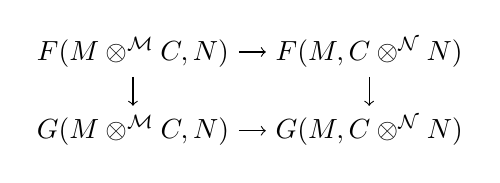
\begin{tikzpicture}
	\node (LT) at (0, 1) {$F(M \otimes^{\cM} C, N)$};
	\node (LB) at (0, 0) {$G(M \otimes^{\cM} C, N)$};
	\node (RT) at (3, 1) {$F(M, C \otimes^{\cN} N)$};
	\node (RB) at (3, 0) {$G(M, C \otimes^{\cN} N)$};
	\draw [->] (LT) -- node [left] {$$} (LB);
	\draw [->] (LT) -- node [above] {$$} (RT);
	\draw [->] (RT) -- node [right] {$$} (RB);
	\draw [->] (LB) -- node [below] {$$} (RB);
	%\node at (0.5, 1) {$\ulcorner$};
	%\node at (1.5, 0.5) {$\lrcorner$};
\end{tikzpicture}.
\end{center}
\end{definition}


\begin{definition}
	Let $\cA$ be a right $\cC$-module category and let $\cB$ be a left $\cC$-module category. The {\em relative Deligne tensor product $\cA \boxtimes_{\cC} \cB$} is the universal linear category admitting a $\cC$-balanced multilinear functor $\boxtimes_{\cC}: \cA \times \cB \to \cA \boxtimes_{\cC} \cB$. That is, there exists a $\cC$-balanced multilinear functor $\boxtimes_{\cC}: \cA \times \cB \to \cA \boxtimes_{\cC} \cB$ which induces, for all linear categories $\cD$, an equivalence between the category of $\cC$-balanced multilinear functors $\cA \times \cB \to \cD$ and the category of linear functors $\cA \boxtimes_{\cC} \cB \to \cD$. 
\end{definition}

If it exists, the Deligne tensor product is unique up to equivalence, and this equivalence is in turn unique up to unique natural isomorphism. Said another way, the 2-category of linear categories representing the Deligne tensor product is either contractible or empty. 

\begin{maintheorem} \label{thm:DelignePrdtOverATCExists}
	Let $\cC$ be a tensor category and let $\cA_{\cC}$ and ${}_{\cC}\cB$ be finite right and left $\cC$-module categories, respectively. Then,
	\begin{enumerate}
		\item The relative Deligne tensor product $\cA \boxtimes_{\cC} \cB$ exists and is a finite linear category;
		\item If $\cA = \Mod{A}{}(\cC)$ and $\cB = \Mod{}{B}(\cC)$, then $\cA \boxtimes_{\cC} \cB \simeq \Mod{A }{B}(\cC)$;

		\item The functor $\boxtimes_{\cC}$ is exact in each variable and satisfies 
		\begin{equation*}
			\Hom_{\cA}(x,x') \otimes \Hom_{\cB}(y, y') \cong \Hom_{\cA \boxtimes_{\cC} \cB} (x \boxtimes_{\cC} y, x' \boxtimes_{\cC} y'),
		\end{equation*}
		\item If $F: \cA \times \cB \to \cD$ is a $\cC$-balanced multilinear functor which is exact in each variable, then it defines an exact functor $\overline{F}: \cA \boxtimes_{\cC} \cB \to \cD$. 
	\end{enumerate} 
\nid Here $\Mod{A}{B}(\cC)$ denotes the category of $A$-$B$-bimodule objects in $\cC$.	
\end{maintheorem}

Equipped with the relative Deligne tensor product and its properties, we can now define the 3-category of interest.

\CSP{Get theorem number.}
\begin{maintheorem}[\cite{3TC}]
	There exists a symmetric monoidal $(3,3)$-category whose objects are the finite rigid tensor categories, whose 1-morphisms are bimodule categories, whose 2-morphisms are bimodule functors, and whose 3-morphisms are bimodule natural transformations. Composition is given by the relative Deligne tensor product of bimodules. The symmetric monoidal structure is given by the usual Deligne tensor product. 
\end{maintheorem}

\subsection{Exact module categories} \label{sec:tc-exact}
% The results here are used in section 4.4 to build adjoints.
In this section we summarize Etingof and Ostrik's theory of exact module categories \cite{MR2119143}.  This theory will be used when we prove that finite tensor categories are Radford objects.   We also prove a new lemma about exactness of Deligne tensor products.

\begin{definition}
	Let $\cC$ be a tensor category. A (left) $\cC$-module category $\cM$ will be called {\em exact} if for any object $m \in \cM$ and  projective object $p \in \cC$, the object $p \otimes m$ is projective in $\cM$. 
\end{definition}

\begin{example}
	If $\cC$ is semisimple, then $\cM$ is an exact module category if and only if it is semisimple.
\end{example}

\begin{example}[{\cite[Example 2.6.5]{EGNO}}] \label{ex:exactness}
	A tensor category $\cC$ is exact when considered as a $\cC$-, $\cC^{mp}$-, or $\cC \boxtimes \cC^{mp}$-module category. 
\end{example}
%\CSP{I think we might want to add some material to this example discussing the alegbra $A = \IHom(1,1) \in \cC \boxtimes \cC^\mp$. }

The following omnibus theorem summarizes the key properties of exact module categories: 
\begin{theorem}[\cite{EGNO}] \label{Thm:ExactModCatOmnibus}
	Let $\cC$ be a tensor category (hence finite and rigid), and let $\cM$, $\cM'$, and $\cM''$ be exact $\cC$-module categories (not assumed to be finite), and let $\cN$ be an arbitrary $\cC$-module category. Then,
	\begin{enumerate}
		\item $\cM$ has enough projectives. \cite[Lemma 2.7.1]{EGNO}
		\item Every projective object in $\cM$  is injective, and vice versa. \cite[Cor 2.7.4]{EGNO}
		\item $\Fun_{\cC}(\cM, \cM')$ is finite \cite[Prop 2.13.5]{EGNO}; in particular $\cM \simeq \Fun_{\cC}(\cC, \cM)$ is finite.
		\item Composition $\Fun_{\cC}(\cM, \cM') \times \Fun_{\cC}(\cM', \cM'') \to \Fun_{\cC}(\cM, \cM'')$ is exact in each variable. \cite[Lemma 2.13.2]{EGNO}		
		\item Every additive (not a priori right exact) module functor $F:\cM \to \cN$ is exact \cite[Prop 2.7.8]{EGNO}. Hence every functor $F \in \Fun_{\cC}(\cM, \cM')$ is exact, and has exact left and right adjoints. Moreover, $\Fun_{\cC}(\cM,\cM)$ is itself a tensor category (in particular finite and rigid). 
	\end{enumerate}
\end{theorem}
%\CD{There are multiple different online documents entitled ``Tensor Categories" by EGNO --- update .bib to have specifying reference, eg url.}

\noindent In fact it is enough to check exactness condition for any collection of projective generators of $\cC$. 

\begin{lemma} \label{lma:Exact_checked_on_proj_gens}
	Let $\cC$ be a tensor category and $\cM$ a finite (left) $\cC$-module category. Let $\cP = \{ p_\alpha \}$ be a fixed collection of jointly generating projective objects of  $\cC$. Then the following are equivalent:
	\begin{enumerate}
		\item for all $m \in \cM$ and all $p_\alpha \in \cP$, the object $p_\alpha \otimes m \in \cM$ is projective;
		\item the $\cC$-module category $\cM$ is exact.
	\end{enumerate}
	(Recall that to say the family $\cP$ is {\em jointly generating} means the functor $\prod_\alpha\cC(p_\alpha, -): \cC \to \Set$ is faithful)
\end{lemma}

\begin{proof}
	It is clear $(2) \Rightarrow (1)$; we prove the converse. Since $\cP$ forms a jointly generating collection of object it follows that for any object $q \in \cC$ there exists a finite sum $p = \oplus_i p_i$ of object of $\cP$ and a surjection $\pi:p \twoheadrightarrow q$. 
	
		 If $q$ is projective, then there exists a section of $\pi$, realizing $q$ as a direct summand of $p$. For every $m \in \cM$, the functor $(-)\otimes m$ is right exact, hence we have an exact sequence
		\begin{equation*}
			p \otimes m \to q \otimes m \to 0.
		\end{equation*}
		 The first map admits a section, and hence $q \otimes m$ is a direct summand of $p \otimes m$. By assumption the later is projective, whence $q \otimes mß$ is projective for every projective $q \in \cC$ and every $m \in \cM$. 
\end{proof}



\begin{definition}
We say that a $\cC$--$\cD$ bimodule category is exact if it is exact as a $\cC \boxtimes \cD^\mp$ module category.
\end{definition}



\begin{theorem}\label{thm:tensor-exactness}
If $\cM$ is an exact $\cC$ module category and $\cN$ is an exact $\cD$ module category, then $\cM \boxtimes \cN$ is an exact $\cC \boxtimes \cD$ module category.
\end{theorem} %This thereorem is new, not stated anywhere because no one needed it.
\begin{proof}
We begin by observing that the Deligne tensor product preserves projective/injective objects in the following sense: if $m \in \cM$ and $n \in \cN$ are both projective objects, then $m \boxtimes n \in \cM \boxtimes \cN$ is also projective. Similarly if $m$ and $n$ are injective, then $m \boxtimes n$ will be injective. This closure property follows directly from Theorem \ref{thm:DelignePrdtOverATCExists}.(4) describing the universal property of the Deligne tensor product. 	
	
Let $\cP$ be the collection of objects of $\cC \boxtimes \cD$ of the form $p \boxtimes q$ for projective objects $p \in \cC$ and $q \in \cD$. Then $\cP$ forms a jointly generating family of projectives. The fact that this family is jointly generating can be seen, for example, from Thm. \ref{thm:EGNO2.11.6}. By Lemma \ref{lma:Exact_checked_on_proj_gens} above, it is enough to check that $(p \boxtimes q) \otimes x$ is projective for every object $x \in \cM \boxtimes \cN$. In other words we wish to show that the following functor is exact:
\begin{equation*}
	\Hom((p \boxtimes q) \otimes x, -) \cong \Hom(x, ({}^*p \boxtimes {}^*q) \otimes(-) ): \cM \boxtimes \cN \to \Vec
\end{equation*}

Note that by our previous observations this follows immediately for primitive tensor products, that is 
 objects of the form $ m \boxtimes n$, for then we have
\begin{equation*}
	(p \boxtimes q) \otimes x = (p \boxtimes q) \otimes (m \boxtimes n) \cong (p \otimes m) \boxtimes (q \otimes n).
\end{equation*}
Hence the desired exactness property also holds for finite direct sums of objects of this type. Moverover, by part (4) of Theorem~\ref{thm:DelignePrdtOverATCExists}, for general $x$ it is enough to restrict to $\cM \times \cN$ and 
verify exactness in each variable separately. We will show exactness in the variable $\cM$; exactness in the second variable follows from an identical argument. 

Thus for general $x$ we begin by considering a fixed object $n \in \cN$ and an exact sequences in $\cM$:
\begin{align*}
	m_1 \to m_2 \to m_3 \to 0. 
%	  n_1 \to n_2 \to n_3 \to 0.
\end{align*}
By \cite[Prop. 2.3]{MR2119143} if $y$ is a projective object in a finite tensor category then ${}^*y$ is also projective. Thus by Theorem \ref{Thm:ExactModCatOmnibus}.(2) the object ${}^*q \otimes n$ and each of the objects ${}^*p \otimes m_i$ are injective, hence for each $i = 1,2,3$ so is the object 
\begin{equation*}
	z_{i} :=  ({}^*p \otimes m_i) \boxtimes ({}^*q \otimes n).
\end{equation*}
Moreover, since the Deligne tensor product is exact and tensoring with objects of $\cC$ is exact (tensoring with appropriate duals gives each adjoint), we have an exact sequences of injective objects of $\cM \boxtimes \cN$:
\begin{equation*}
	z_1 \to z_2 \to z_3 \to 0.
\end{equation*}

Finally it follows from Theorem \ref{thm:EGNO2.11.6} that for every object $x \in \cM \boxtimes \cN$ there exists a short exact sequence
\begin{equation*}
	0 \to x'' \to x' \to x \to 0
\end{equation*}
 such that $x'$ is a finite direct sum of objects of the form $m \boxtimes n$. Putting these facts together we obtain the commutative diagram in Figure \ref{fig:exact-mod-cat-exact}. 
%\CSP{I think I don't want zeros on the left-most side. I should double check that they aren't needed.}
\begin{figure}[htbp]
	\begin{center}
		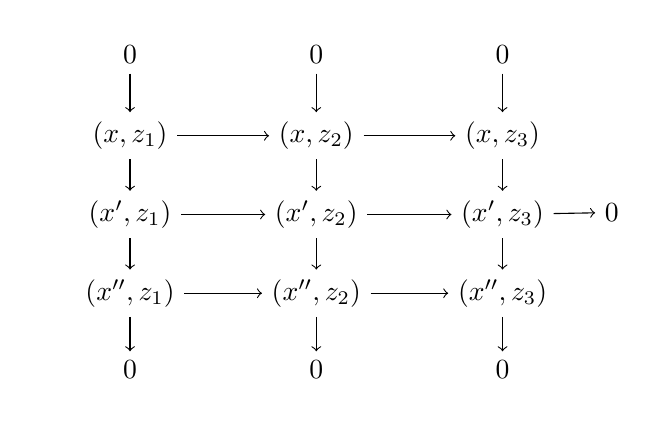
\begin{tikzpicture} \matrix (m) [matrix of math nodes, row sep={1cm,between origins}] {
		 &[0.5cm] 0 &[1cm] 0 &[1cm] 0 &[0.5cm]  \\ 
		 & \Hom(x, z_1) & \Hom(x, z_2) & \Hom(x, z_3) & \\ 
		 & \Hom(x', z_1) & \Hom(x', z_2) & \Hom(x', z_3) & 0 \\
		 & \Hom(x'', z_1) & \Hom(x'', z_2) & \Hom(x'', z_3) & \\
		& 0 & 0 & 0 & \\
		};
		\foreach \sourcerow/ \sourcecol / \targetrow / \targetcol in 
			{1/2/2/2, 1/3/2/3, 1/4/2/4, % first row of down arrows
			2/2/3/2, 2/3/3/3, 2/4/3/4,  % second row of down arrows
			3/2/4/2, 3/3/4/3, 3/4/4/4,  % third row of down arrows
			4/2/5/2, 4/3/5/3, 4/4/5/4,  % fourth row of down arrows
			%2/1/2/2, 
			2/2/2/3, 2/3/2/4, % first row of horiz arrows
			%3/1/3/2, 
			3/2/3/3, 3/3/3/4, 3/4/3/5, % second row of horiz arrows
			%4/1/4/2, 
			4/2/4/3, 4/3/4/4} % third row of horiz arrows
			\draw [->] (m-\sourcerow-\sourcecol) -- (m-\targetrow-\targetcol);
		\end{tikzpicture}
	\end{center}
	\caption{A digram helping show the product of exact module categories is exact.}
	\label{fig:exact-mod-cat-exact}
\end{figure}
The columns are exact because each of the objects $z_i$ is injective. The middle row is exact because $x'$ is a finite direct sum of primitive objects. 

A diagram chase (essentially a variation on the snake lemma applied to the middle rows) shows that we always have a short exact sequence
\begin{equation*}
	 \Hom(x, z_1) \to \Hom(x, z_2) \to \Hom(x, z_3) \to 0
\end{equation*}
and hence $\Hom((p \boxtimes q) \otimes x, -)$ is right exact and $(p \boxtimes q) \otimes x$ is projective. 
%\NScomm{Hrm, I think my proof of this may have a hole...}
\end{proof}



\subsection{Dual bimodule categories} \label{sec:examples_of_bimods}

In this section we define some notation for producing new bimodule categories from old ones, and prove several technical lemmas allowing us to manipulate these bimodules easily.  Most of these are closely analogous to simple constructions of bimodules over algebras.  In particular, we prove Lemma \ref{Lma:FunctorsAsATensorPdt}, which shows that a certain relative Deligne tensor product is equivalent to a functor category.  Much as $V \otimes V^\vee \cong \mathrm{End}(V)$ plays the key role in showing that finite-dimensional vector spaces are $1$-dualizable \cite[Ex. 1.1.9]{lurie-ch}, this lemma plays the key role in proving the $2$-dualizability of finite tensor categories.

As ${}_A A_A$ denotes the identity bimodule, so ${}_\cC \cC_{\cC}$ will denote the identity bimodule category.  Our first source of examples comes from turning left actions by $\cC$ into right actions by $\cC^\mp$.  This is analogous to replacing a left action of an algebra $A$ by a right action of the opposite algebra.

\begin{definition}
Every left $\cC$-module category ${}_\cC \cM$ is naturally a right $\cC^{mp}$-module category, and we will denote this new module category by $\cM_{\cC^{mp}}$.  More generally, if ${}_{\cC \boxtimes \cD} \cM_{\cE}$ is a $(\cC \boxtimes \cD)$-$\cE$ bimodule then $\cM$ is also a $\cC$-$(\cD^\mp \boxtimes \cE)$ bimodule category, which we will denote ${}_{\cC}\cM_{\cD^\mp \boxtimes \cE}$.
\end{definition}

We will be particularly interested in the modules $\cC_{\cC \boxtimes \cC^\mp}$ and ${}_{\cC^\mp \boxtimes \cC} \cC$ obtained by applying this procedure to the identity bimodule ${}_\cC \cC_\cC$.  Note that if you move both actions on ${}_\cC \cC_\cC$ to the opposite side, you obtain a bimodule ${}_{\cC^\mp}\cC_{\cC^\mp}$, which is in fact the identity bimodule on $\cC^\mp$.

\begin{example}[The category of Hopf bimodules] \label{Ex:Hopf_bimod}
	Let $\cC$ be a tensor category, and consider it as a left $\cC \boxtimes \cC^\mp$-module category. Let $A = \IHom(1,1)$ be the enriched endomorphism object of $1 \in \cC$ (cf. section \ref{sec:tc-bimod}); $A$ is an algebra object in $\cC \boxtimes \cC^\mp$. 
The object $1 \in \cC$ is a $\cC$-projective $\cC$-generator (cf. example \ref{ex:rigid_all_C-proj}) and hence by Lemma \ref{lma:module-adjoint} and Theorem \ref{thm:C-module-Embedding} the functor $\IHom(1, -)$ induces an 
 equivalence of left $\cC \boxtimes \cC^\mp$-module categories:
	\begin{equation*}
		{}_{\cC \boxtimes \cC^\mp} \cC \simeq \Mod{}{A}(\cC \boxtimes \cC^\mp).
	\end{equation*} 
In particular it follows that every object $x \in \Mod{}{A}(\cC \boxtimes \cC^\mp)$ may be written as 
\begin{equation*}
	x \cong (c \boxtimes 1) \otimes A
\end{equation*}
for some object $c \in \cC$, unique up to isomorphism. 
\CSP{do we want to define the distinguished invertible object?}
\end{example}

Just as modules over algebras can be twisted by algebra maps, we can twist module categories by tensor functors.

\begin{definition}
Suppose that $\cM$ is a $\cC$--$\cD$ bimodule category, and that $\cF: \cC' \rightarrow \cC$ is a tensor functor, let
${}_{\langle \cF \rangle} \cM$ denote the $\cC'$--$\cD$ bimodule where the new action is $c' \cdot m \cdot d = \cF(c') \otimes m \otimes d$, together with the obvious natural isomorphisms.  For a functor $F: \cD' \ra \cD$, define $\cM_{\langle \cF \rangle}$ similarly.
\end{definition}

Note that ${}_{\langle \cF \rangle} \cC_\cC \boxtimes_{\cC} {}_{\cC} \cM_\cD \cong {}_{\cC} ({}_{\langle \cF \rangle} \cM)_\cD$.  Note also ${}_{\langle \cF \rangle \langle \cG \rangle} \cM \cong {}_{\langle \cF \otimes \cG \rangle} \cM$, while $\cM_{\langle \cF \rangle \langle \cG \rangle} \cong  \cM_{\langle \cG \otimes \cF \rangle}$.  Twisting on the left therefore gives a tensor functor from the $2$-category of finite tensor categories, tensor functors, and tensor natural transformations to $\TC$: it is the identity of objects and sends the morphism $\cF: \cC \rightarrow \cD$ to the bimodule ${}_{\cC} ({}_{\langle \cF \rangle} \cD)_{\cD}$.  Twisting on the right gives a functor from the 1-morphism-opposite of the $2$-category to $\TC$.

\begin{lemma} \label{lem:BimoduleToFunctor}
Suppose that $\cC$ and $\cD$ are tensor categories and $\cF: \cC \rightarrow \cD$ is a tensor functor.
Giving a bimodule isomorphism $\alpha:{}_{\cC} ({}_{\langle \cF \rangle} \cD)_\cD \rightarrow {}_{\cC} ({}_{\langle \cG \rangle} \cD)_\cD$ is the same data as giving an invertible object $D \in \cD$ and a natural isomorphism $\varphi_x: \cF(x) \rightarrow D^{-1} \otimes \cG(x) \otimes D$.
\end{lemma}
\begin{proof}
The functor $\alpha$ is, in particular, a right $\cD$-module functor from $\cD$ to $\cD$ and thus is given by tensoring on the left by an object $D \in \cD$, $\alpha(d) \cong D \otimes d$. The object $D$ is the image of $1$, and is $\otimes$-invertible since $\alpha$ is an isomorphism. The left $\cC$-module structure on $\alpha$ may be expressed as a system of natural isomorphisms
\begin{equation*}
	D \otimes \cF(c) \otimes d \cong \alpha (c \cdot d) \cong c \cdot \alpha(d) \cong \cG(c) \otimes D \otimes d.
\end{equation*}
and hence is equivalent to the data of $\varphi$. 
\end{proof}

The bimodule category ${}_\cD \Fun_\cC(\cM,\cC)_\cC$ will play a central role in our dualizability calculations, and it will be convenient to have several alternative descriptions of this bimodule category.

\begin{definition} \label{def:Dual_bimodule_notation}
For a bimodule category ${}_\cC \cM_\cD$, let $\cM^*$ denote a $\cD$--$\cC$ bimodule category defined as follows.  The underlying category of $\cM^*$ is the category $\cM^{\op}$. An object $m \in \cM$ is denotes $m^*$ when viewed as an object of $\cM^* = \cM^\op$.  The $\cD$--$\cC$ bimodule category structure is given by
\begin{equation*}
	d\cdot m^* \cdot c := ({}^*c \otimes m \otimes {}^*d)^*
\end{equation*}
Similarly, let ${}^*\cM$ denote the $\cD$--$\cC$ bimodule category whose underlying category is $\cM^{\op}$ and whose action is given by $d\cdot {}^*m \cdot c := {}^*(c^* \otimes m \otimes d^*)$.  
\end{definition}

Recall that a $\cC$-module category $\cM$ is called {\em exact} if $p \otimes m \in \cM$ is projective whenever $p \in \cC$ is projective.  See Appendix~\ref{sec:tc-exact} for a summary of the theory of exact module categories.

\begin{lemma}
Suppose that $\cM$ is an exact $\cC$-module category, that $\cF: \cC \rightarrow \cC^\mop$ is an equivalence of tensor categories, and that $\cM^{\op}$ is the mod-$\cC$ given by $m \cdot c = \cF(c) \otimes m$.  Then $\cM^\op$ is an exact mod-$\cC$.
\end{lemma}
\begin{proof}
By \cite[Prop. 2.3]{MR2119143} and \cite[Corollary 3.6]{MR2119143} the injective objects and projective objects agree in $\cC$ and in $\cM$.  Now consider $x$ a projective object in $\cC$ and $m$ an arbitrary object in $\cM^\op$, and look at $m \cdot c = \cF(c) \otimes m$.  Since $\cF(c)$ is projective in $\cC^\mop$ it is also injective in $\cC^\mop$, and hence projective in $\cC$.  Hence $\cF(c) \otimes m$ is projective in $\cM$, hence injective in $\cM^\op$, and thus projective in $\cM^\op$.
\end{proof}

\begin{corollary} \label{cor:adjoint-exactness}
Suppose that $\cM$ is an exact $\cC$--$\cD$ bimodule category, then $\cM^*$ and ${}^*\cM$ are exact $\cD$--$\cC$ bimodule categories.
\end{corollary}


\begin{definition}
	Let ${}_{\cC}\cM_\cD$ be a $\cC$-$\cD$ bimodule category and let ${}_{\cC}\cN_\cE$ be a $\cC$-$\cE$ bimodule category. Temporarily breaking from our convention of only considering right exact functors, let	 $\Fun^L_{\cC}(\cN, \cM)$ denote the category of left exact $\Vect$-enriched $\cC$-module functors (which are not necessarily right exact). This is naturally a $\cD$-$\cE$ bimodule category. We may similarly define bimodule categories of left exact right module functors. 
\end{definition}

\begin{lemma}
If ${}_{\cC}\cM_\cD$ is a $\cC$-$\cD$ bimodule category and ${}_{\cC}\cN_\cE$ is a $\cC$-$\cE$ bimodule category, then taking right adjoints gives an equivalence of $\cD$-$\cE$ bimodule categories 
from $\Fun_{\cC}(\cM, \cN)$ to ${}^*\Fun^L_{\cC}(\cN, \cM)$.
% where $\Fun^L_\cC$ denotes {\em left exact} $\Vect$-enriched module functors.  
Similarly, if $\cM$ is a $\cC$-$\cD$ bimodule category and $\cN$ is a $\cE$-$\cD$ bimodule category, then taking right adjoints gives an equivalence of $\cC$-$\cE$ bimodule categories from ${}^*\Fun_{\cD}(\cM, \cN)$ to $\Fun^L_{\cD}(\cN, \cM)$. 
\end{lemma}
\begin{proof}
	We will prove the first statement as the second follows from a similar argument. 
We have already seen in Lemma \ref{lma:module-adjoint} that the adjoint of a module functor has a canonical module functor structure.  Furthermore, taking left adjoints is clearly an equivalence of the relevant functor categories; the inverse equivalence is given by taking right adjoints. Thus we need only check that the $\cD$-$\cE$ bimodule structures agree under this equivalence.  First note that taking adjoints reverses the order of composition. Second, note that, as mentioned after Lemma~\ref{lma:RigidIsExact}, the right adjoint of right multiplication by $e$ is right multiplication by $e^*$.
\end{proof}

\begin{lemma} \label{lem:dual-formula-for-adjoints}
For a bimodule category ${}_\cC \cM_\cD$, we have equivalences $\cM^* \simeq \Fun_{\cD}(\cM, \cD)$ and ${}^*\cM \simeq \Fun_{\cC}(\cM, \cC)$.
\end{lemma}
\begin{proof}
By the previous lemma, $\Fun_{\cC}(\cM, \cC) \simeq {}^*\Fun_{\cC}^L(\cC, \cM)$.  Any left $\cC$-module functor $\cF: \cC \ra \cM$ is given by $c \mapsto c \otimes \cF(1)$; this functor is a right adjoint (see the comments after Lemma~\ref{lma:RigidIsExact}) and therefore is left exact.  It follows that ${}^*\Fun_{\cC}^L(\cC, \cM)$ is ${}^* \cM$ as desired.
\end{proof}

The following lemma is crucial for our results. \CD{Explain this sentence.}
It is close in spirit to \cite[Prop. 3.5 and Rmk. 3.6]{0909.3140} and \cite[Thm. 3.20]{0911.4979}, however these previous result assume semisimplicity over an algebraically closed field of characteristic zero, and moveover both statements contain minor inaccuracies regarding the equivalence as bimodule categories. See Remark \ref{rmk:Deligne_pdt_as_mod_functor} for details and the corrected version of \cite[Rmk. 3.6]{0909.3140} and \cite[Thm. 3.20]{0911.4979}.
\CSP{How do these comments read? Too harsh?} 
\CD{Perhaps rephrase this paragraph now that it is so close to \ref{rmk:Deligne_pdt_as_mod_functor}}

\begin{lemma} \label{Lma:FunctorsAsATensorPdt}
	If $\cC$ is a tensor category and $\cM$ and $\cN$ are finite left $\cC$-module categories then the natural functor induces an equivalence
	\begin{equation*}
		\Fun_\cC(\cM, \cC) \boxtimes_\cC \cN \simeq \Fun_\cC(\cM,\cN).
	\end{equation*}
	Here $\Fun_\cC$ denotes the category of (right exact) $\cC$-module functors. 
	Moreover, if $\cM$ and $\cN$ are bimodule categories, then the above equivalence is a bimodule equivalence. 
\end{lemma}

\begin{proof}
	The last sentence follows since in that case the natural functor is a bimodule functor. By Theorem \ref{thm:EGNO2.11.6}, there exist algebra objects $A, B \in \cC$ and equivalences $\cM \simeq \Mod{}{A}(\cC)$ and $\cN \simeq \Mod{}{B}(\cC)$. We first show that both sides of the above equation are naturally equivalent to $\Mod{A}{B}(\cC)$. The equivalence $\Fun_\cC(\cM, \cN) \simeq \Mod{A}{B}(\cC)$ (established in \cite[Prop 2.12.2]{EGNO}) can be seen by following the classical proof. A bimodule clearly gives rise to such a functor, and given a functor $f$, we obtain an $A$-$B$-bimodule $f(A)$. By $\cC$-linearity $f(X \otimes A) \cong X \otimes f(A)  \cong (X \otimes A) \otimes_A f(A) $ is determined on free $A$-modules. Since every object of $\cM$ may be written as a (canonical) coequalizer of free $A$-modules,
	\begin{equation*}
		M \leftarrow M \otimes A \leftleftarrows M \otimes A \otimes A
	\end{equation*} 
the functor $f$ is equivalent to the one determined by the bimodule $f(A)$. Thus the natural map  $\Mod{A}{B}(\cC) \to \Fun_\cC(\cM, \cN)$ is essentially surjective. The above argument also shows it is fully-faithful, so that $\Fun_\cC(\cM, \cN) \simeq \Mod{A}{B}(\cC)$, which in particular shows $\Fun_\cC(\cM, \cC) \simeq \Mod{}{A}(\cC)$. Now the result follows from Theorem \ref{thm:DelignePrdtOverATCExists}.
%Tensoring a left $A$-module and a right $B$-module gives a canonical $\cC$-balanced bilinear functor 
%\begin{equation*}
%	T: \Mod{A}{}(\cC) \times \Mod{}{B}(\cC) \to \Mod{A}{B}(\cC). 
%\end{equation*}
%To complete the proof we must show this induces an equivalence,
%\begin{equation*}
%	\Mod{}{A}(\cC) \boxtimes_\cC \Mod{B}{}(\cC) \simeq \Mod{B}{A}(\cC).
%\end{equation*}
%When $\cC = \Vect$, this is classical. More generally we must show that the right-hand-side has the desired universal property. For this purpose let $F:\Mod{}{A}(\cC) \times \Mod{B}{}(\cC) \to \cA$ be a $\cC$-balanced bilinear functor. There is a unique right exact linear functor $\overline F: \Mod{B}{A}(\cC) \to \cA$ such that $F = \overline{F} \circ T$ which is defined as follows. On free bimodules $A \otimes X \otimes B \cong T(A \otimes X, B)$, we necessarily have $\overline{F}(A \otimes X \otimes B) \cong F(A \otimes X, B)$. Since $\overline{F}$ is right exact and every $A$-$B$-bimodule is a coequalizer of free $A$-$B$-bimodules, the result follows. 	
\end{proof}
%\CD{Did that really prove that the natural functor is an equivalence, or just that there is an equivalence?}

\begin{remark} \label{remark-tensorasfunctors}
If $\cM$ and $\cN$ are right $\cD$-modules, then we have that $\cN \boxtimes_\cD \Fun_{\cD}(\cM,\cD) \simeq \Fun_{\cD}(\cM,\cN)$, and again if $\cM$ and $\cN$ are bimodule categories, then this equivalence is a bimodule equivalence. 
\end{remark}

%%%%%%%%%


\begin{remark} \label{rmk:Deligne_pdt_as_mod_functor}
Combining Lemmas \ref{lem:dual-formula-for-adjoints} and \ref{Lma:FunctorsAsATensorPdt} and Remark~\ref{remark-tensorasfunctors}, we learn that if $\cM$ is a finite $\cD$-$\cC$ bimodule and $\cN$ is a finite $\cC$-$\cE$ bimodule, then 
\begin{equation*}
	\cM \boxtimes_\cC \cN \simeq {}^*(\cM^*) \boxtimes_\cC \cN \simeq \Fun_{\cC\text{-mod}}(\cM^*,\cN)
\end{equation*}
as $\cD$-$\cE$ bimodule categories.   Similarly, 
\begin{equation*}
	\cM \boxtimes_{\cC} \cN \simeq \cM \boxtimes_\cC ({}^*\cN)^* \simeq \Fun_{\text{mod-}\cC}({}^*\cN,\cM)
\end{equation*}
as $\cD$-$\cE$ bimodule categories. 

	 These bimodule category equivalences are a correction of \cite[Remark 3.6]{0909.3140} and \cite[Thm. 3.20]{0911.4979}, both of which give $\cM^\op$ the structure of a $\cC$-$\cD$ bimodule category, which differs by twisting the $\cD$-action by the double dual functor. Note also that the proof of \cite[Thm. 3.20]{0911.4979} is incomplete. In particular it relies on \cite[Lma. 3.21]{0911.4979} which is false. A counterexample is given by setting $\cC = \Vect_G$, the category of $G$-graded vector spaces for a fixed finite group $G$, and $\cM = \cN = \Vect$. The forgetful functor $U:\cC \to \Vect$ which forgets the grading is a tensor functor and endows $\cM$ and $\cN$ with the structure of right and left $\cC$-module categories, respectively. In this case \cite[Lma. 3.21]{0911.4979} asserts an equivalence between $\cM \boxtimes \cN \simeq \Vect \boxtimes \Vect \simeq \Vect$ and $\Fun_\cC(\Vect, \Vect) \simeq \Rep(G)$, which is false unless $G$ is the trivial group.
\end{remark}

\begin{remark}
	The notation of Definition \ref{def:Dual_bimodule_notation} is consistent with our earlier conventions, specifically the convention that the composition order of tensor products is from left to right; indeed the bimodule ${}^*\cM$ is the both the left adjoint and the left dual of $\cM$, while $\cM^*$ is both the right adjoint and right dual. (c.f. Definitions \ref{def:Adjoints} and \ref{def:rigid} in Section \ref{sec:conventions}). 
\end{remark}

\begin{warning}
Because the left dual on $\cC$ becomes a right dual on $\cC^\mp$ and vice-versa, taking the left or right dual of a bimodule does not commute with moving the tensor categories acting from one side to the other.  Instead, we have ${}_\cD ((\cM_{\cC^\mp \boxtimes \cD})^*)_\cC \simeq {}_{\langle \mathfrak{r r} \rangle}(({}_\cC \cM_\cD)^*)$ where $\mathfrak{r}$ is the right dual functor.%\NS{Someone should double-check left vs. right here} % It is now correct - CSP. 
\end{warning}

Theorem \ref{thm:EGNO2.11.6} implies that in a precise sense all module categories are categories of modules. Specifically if $A$ is an algebra object in the tensor category $\cC$, then $\Mod{}{A}(\cC)$ and $\Mod{A}{}(\cC)$ are left and right $\cC$-module categories, respective (see example \ref{ex:ModulesAreModules}). We will end this section with a few lemmas concerning module categories of this type based on \cite{0404504}[\S 3].

\begin{lemma}
	Let $A$ and $B$ be algebra objects in the tensor category $\cC$. Let $M$ be an $A$-$B$-bimodule (which is, in particular, an object in $\cC$). Then ${}^{**}A$ and $B^{**}$ are naturally algebra object of $\cC$, $M^*$ is naturally a $B^{**}$-$A$-bimodule, and ${}^*M$ is naturally a $B$-${}^{**}A$-bimodule. Moreover these identifications induce equivalences of linear categories:
	\begin{equation*}
		\Mod{B^{**}}{A}(\cC) \simeq \Mod{A}{B}(\cC) \simeq \Mod{B}{{}^{**}A}(\cC).
	\end{equation*}
\end{lemma}

\begin{proof}
	The left and right double dual functors are equivalences of tensor categories hence preserve algebra objects. Consider the action map $\mu:A \otimes M \otimes B \to M$. Applying the (anti-monoidal contravariant) automorphism $(-)^*$, this becomes
	\begin{equation*}
		M^* \to B^* \otimes M^* \otimes A^*,
	\end{equation*}
	which induces a new action map:
	\begin{equation*}
		B^{**} \otimes M^* \otimes A \to M^*.
	\end{equation*}
	The case for left duals is similar. 
\end{proof}

\begin{lemma}
	Let $A$ be an algebra object in the tensor category $\cC$. Then we have an equivalences of $\cC$-module categories: 
	\begin{align*}
		(\Mod{}{A}(\cC))^* & \simeq \Mod{A^{**}}{}(\cC) \\
		(L)^* & \mapsto L^*.
	\end{align*}
	Here the star of $(L)^*$ on the left side is an abstract symbol which is used to denote objects of $(\Mod{}{A}(\cC))^*$ (cf. Def. \ref{def:Dual_bimodule_notation}), while $L^*$ on the right side denotes the right dual of $L$ as an object of $\cC$. Similarly we have a $\cC$-module equivalence $(\Mod{A}{}(\cC))^* \simeq \Mod{}{A}$.	
\end{lemma}

\begin{proof}
	The existence of the equivalence follows immediately from the previous lemma, and it is routine to check the compatibility of the $\cC$-module structures.  
\end{proof}

\subsection{Separable module categories and separable tensor categories} \label{sec:tc-separable}
In characteristic zero, the collection of fusion categories and their semisimple bimodule categories have many good closure properties.  For example, M\"uger proves that the Drinfel'd center  of a fusion category is fusion \cite[Theorem 3.16]{MR1966525} and Etingof--Nikshych--Ostrik show that functor categories between semisimple module categories over fusion categories are semsimple and hence (because all relative Deligne tensor products can be expressed as functor categories) semisimplicity is preserved by relative Deligne tensor product \cite[Theorem 2.16]{MR2183279}.  However, it is well-known that these results break down in non-zero characteristic.  This happens for two distinct reasons: first, fusion categories of global dimension zero behave poorly, and, second, (as observed by Kuperberg \cite[Question 5.1]{MR1995781}) if you work over a non-perfect field there are problems related to inseparable field extensions.

In this section, we introduce a new notion of separability for module categories and tensor categories that provides the right setting for generalizing the results of M\"uger and Etingof--Nikshych--Ostrik to characteristic $p$.  This theory is a generalization of the classical notion of a separable algebra \cite{???}.   This section was inspired by a suggestion of Ostrik, the results of \cite[\S 2.4]{1009.2117} for fusion categories over $\mathbb{C}$, and by the appearance of separability in the classification of $2$-dimensional local field theories \cite{schommer-pries-thesis}.

\begin{definition}
	Let $A$ be an algebra object in a finite tensor category $\cC$. The multiplication map $\mu: A \otimes A \to A$ may be viewed as a morphism of $A$-$A$-bimodule objects in $\cC$. We will say that $A$ is {\em separable} if the multiplication map splits as a map of $A$-$A$-bimodules. 
\end{definition}

\begin{remark}
	A (right exact) monad $T$ acting on a $\cC$-module category $\cM$ is an algebra object in the tensor category $\Fun_\cC(\cM, \cM)$. Thus the above definition also yields the notion of {\em separable monad}. 
\end{remark}

\begin{remark}
	When $\cC = \Vect_k$, the notion of a separable algebra object $A$ in $\cC$ is the same notion as a separable algebra in the classical sense (that is, an algebra $A$ that is projective as an $A$--$A$ bimodule). Over a perfect field --- such as a finite field, an algebraically closed field, or a field of characteristic $0$ --- the algebra $A$ being separable is equivant to $A$ being a finite-dimensional semisimple $k$-algebra; more generally it is a stronger condition. 
	\CSP{get references to classical notion of separability}
\end{remark}

\begin{theorem} \label{thm:SepModCats}
	Let $\cC$ be a  semisimple tensor category and let $\cM$ be a finite right $\cC$-module category. Then the following are equivalent:
	\begin{enumerate}
		\item $\cM_\cC \simeq \Mod{A}{}(\cC)$, where $A$ is a separable algebra in $\cC$;
		\item $\cM_\cC \simeq \Mod{A}{}(\cC)$, where $A$ is an algebra in $\cC$ that is projective as an $A$-$A$-bimodule;
		\item The identity functor is a projective object of $\Fun_\cC(\cM, \cM)$;
		\item $\Fun_\cC(\cM, \cM)$ is a semisimple category. 
	\end{enumerate}
	Moreover if any of these conditions is satisfied, then $\cM$ is semisimple, hence exact as a $\cC$-module category. The analogous results hold for left $\cC$-module categories as well. 
\end{theorem}


\begin{proof}
	The last sentence is clear since we may switch left/right actions by taking the monoidally-opposite category.
	The proof of Lemma \ref{Lma:FunctorsAsATensorPdt} shows that $\Fun_\cC(\cM, \cM) \simeq \Mod{A}{A}(\cC)$, thus we have clear implications (4) $\Rightarrow$ (3) $\Leftrightarrow$ (2) $\Rightarrow$ (1). We will show that (1) $\Rightarrow$ (4), that is if $A$ is separable, then $\Mod{A}{A}(\cC)$ is a semisimple category. 
	
	Recall that if $F: \cA \leftrightarrows \cB: G$ is an adjunction between abelian categories and the right adjoint $G$ is also right exact, then $F$ sends projective objects to projective objects. This is true because
	\begin{equation*}
		\Hom(F(P), -) \cong \Hom(P, G(-))
	\end{equation*}
	is a right-exact functor. In particular this applies to the free-forget adjunction between $A$-$A$-bimodules and objects of $\cC$. As every object of $\cC$ is projective (since $\cC$ is semisimple) we have that every free $A$-$A$-bimodule is also projective in $\Mod{A}{A}(\cC)$. 
	
Let $s: {}_AA_A \to {}_AA \otimes A_A$ be a bimodule splitting of the multiplication map. For every $A$-$A$-bimodule $X$ we have an induced $A$-$A$-bimodule map
\begin{equation*}
	X \cong A \otimes_A X \otimes_A A 
	\xra{s \otimes_A 1 \otimes_A s} (A \otimes A) \otimes_A X \otimes_A (A \otimes A) \cong A \otimes X \otimes A,
\end{equation*}  	
which splits the canonical action map. Thus $X$ is a direct summand of the free bimodule $A \otimes X \otimes A$. As this latter is projective, $X$ is projective. Thus $\Mod{A}{A}(\cC)$ is semisimple, and (1) $\Rightarrow$ (4). 
	
Finally if $Y \in \cM \simeq \Mod{A}{}(\cC)$ is a left $A$-module, then $s \otimes_A 1: Y \cong A \otimes_A Y \to (A \otimes A) \otimes_A Y \cong A \otimes Y$ realizes $Y$ as a direct summand of a free $A$-module. Again since $\cC$ is semisimple, free $A$-modules are necessarily projective. Thus $Y$ is projective. Hence $\cM$ itself is semisimple.  	
\end{proof}

\begin{definition}
	If any of the equivalent conditions of Theorem \ref{thm:SepModCats} are satisfied, then we will say that $\cM$ is a {\em separable} module category. If $\cM$ is a $\cC$-$\cD$-bimodule category then we will say $\cM$ is separable if it is separable over both $\cC$ and $\cD$ independently. 
\end{definition}

A linear category $\cC$ is separable (as a $\Vect$-module) if and only if it can be realized as a category of algebras over a separable algebra.  Thus $\Vect$-separability is well-understood.   $\Vect$-separability implies semisimplicity, and over a perfect field it is equivalent to semisimplicity.  More generally, each simple object $X$ in a semisimple category $\cC$ has a division ring of endomorphisms $D_X$ with center $K_X$, and $\cC$ is $\Vect$-separable if and only if $K_X/k$ is a finite separable field extension for all $X$.  Equivalently, a linear category is $\Vect$-separable if and only if it is absolutely semisimple in the sense that the category remains semisimple under arbitrary base changes.  Since the word ``separable" is somewhat overloaded in this section we will say ``absolutely semisimple" instead of ``$\Vect$-separable".

\begin{theorem} \label{thm:compositeOfSep}
	If ${}_\cB\cM_\cC$ and ${}_\cC\cN_\cD$ are separable bimodule categories over semisimple tensor categories, then $\cM \boxtimes_{\cC} \cN$ is a separable $\cB$-$\cD$-bimodule category.
\end{theorem}

\begin{proof}
	As separability is a condition on each module structure separately, it is enough to check that $\cM \boxtimes_{\cC} \cN$ is separable as a $\cB$-module category. Our assumptions give the following identifications:
\begin{itemize}
	\item $\cM \simeq \Mod{}{A}(\cB)$ as left $\cB$-module categories for a separable algebra $A$ in $\cB$;
	\item $\cM \simeq \Mod{B}{}(\cC)$ as right $\cC$-module categories for a separable algebra $B$ in $\cC$;
	\item $\cN \simeq \Mod{}{C}(\cC)$ as left $\cC$-module categories for a separable algebra $C$ in $\cC$;
	\item $\cM \boxtimes_{\cC} \cN \simeq \Mod{B}{C}(\cC)$
\end{itemize}
Thus $\cM \boxtimes_{\cC} \cN$ is equivalent to the category of algebras for the separable monad $T = (-) \otimes C$ acting on $\cM$. Moreover $T$ is an algebra in $\Fun_{\cB}(\cM, \cM)$ (i.e. a monad) because the left $\cB$-action on $\cM$ commutes up to coherent natural isomorphism with the right $\cC$-action.  It follows that there is the structure of an algebra on the object $T(A) \in \cB$. The multiplication is given by,
\begin{equation*}
	T(A) \otimes T(A)  \simeq T( T(A) \otimes A)  \xra{T(\textrm{action})} T^2(A) \to T(A),
\end{equation*}
where the first equivalence comes from left $\cB$-linearity of $T$, the next map comes from the action map on $T(A)$ (that is, $T(A) \in \cM \simeq \Mod{}{A}(\cB)$ has a right $A$-action), and the final map is one of the structure maps of the monad $T$. The unit of $T(A)$ is defined similarly. 

One verifies that the the unit map $A \to T(A)$ is homomorphism of algebras in $\cB$. Moreover as $T$ is right exact and $\cB$-linear, we have $T(m) \cong m \otimes_A T(A)$ for all $m \in \Mod{}{A}(\cB) \simeq \cM$. Thus the category of $T$-algebras in $\Mod{}{A}(\cB)$ is nothing more then the category of right $T(A)$-modules in $\cB$.  Hence we have shown $\cM \boxtimes_{\cC} \cN \simeq \Mod{}{T(A)}(\cB)$ as left $\cB$-module categories. It remains to show that $T(A)$ is a separable algebra in $\cB$.

As both $A$ and $T$ are separable, we have splittings of the canonical multiplication maps, $s: A  \to A \otimes A$, and $\sigma:T \to T^2$. These induce a splitting of the $T(A)$-multiplication map:
\begin{equation*}
	T(A) \stackrel{\sigma}{\to} T^2(A) \xra{T(1 \otimes_A s)} T( T(A) \otimes A) \cong T(A) \otimes T(A).
\end{equation*}
Thus $T(A)$ is separable.
\end{proof}

Note that $\cC$ is always seperable as a $\cC$-$\cC$ bimodule category.  However, we will often need to consider $\cC$ as a $\cC \boxtimes \cC^\mp$--$\Vect$ bimodule as well.  This suggests the following definition.

\begin{definition}
	A semisimple tensor category is {\em separable} if it is separable as a $\cC \boxtimes \cC^\mp$--$\Vect$-bimodule category.  
\end{definition}


\begin{definition}
	Let $\cC$ be a finite tensor category. The {\em center} of $\cC$ is the linear category $\cZ(\cC) := \Fun_{\cC \boxtimes \cC^\mp}(\cC, \cC)$.
\end{definition}

With this definition, observe that Theorem~\ref{thm:SepModCats} implies the following.

\begin{corollary} \label{cor:Sep=semisimplecenter}
	The following are equivalent for an absolutely semisimple finite tensor category $\cC$.
	\begin{enumerate}
		\item $\cC$ is separable;
		\item The center $\cZ(\cC)$ is semisimple.
	\end{enumerate} 
\end{corollary}

\begin{theorem}
Separable finite tensor categories, finite absolutely semisimple separable bimodule categories, bimodule functors, and bimodule natural transformations, form a symmetric monoidal $3$-subcategory of $\TC$.
\end{theorem}
\begin{proof}
This follows from applying the previous theorem a bunch of times.  $\Vect$ separability of the bimodule categories is needed for the monoidal structure
\end{proof}


\subsection{Fusion categories and separability} \label{sec:tc-fusion}

The goal of this section is to show that under nice circumstances of classical interest  separability is easy to verify. In this section we restrict ourselves to working over an algebraically closed field. Recall that a (finite rigid) tensor category is called \emph{fusion} if it is semisimple and if the unit object is simple. Since we are working over an algebraically closed field this implies that the endomorphisms of the unit object, indeed any simple object, are canonically isomorphic to the ground field. 

Fusion tensor categories have an invariant known as the \emph{global dimension} which lives in the ground field. (We will recall its definition momentarily). It is generally known that the when the global dimension is non-zero, then the center $\cZ(\cC)$ is semisimple. This is shown for example in \cite[Prop. 3.10]{MR1966525} under the assumption that the fusion category is spherical, and it is shown in \cite[Thm. 2.15]{MR2183279} without assuming sphericality but with the assumption that the ground field is characteristic zero (but see also section 9 of that same paper). 
%%%
%\CSP{Does M\"uger's proof depend on sphericality? I checked that you always get that the center is rigid (M\"uger Prop 3.9) and this doesn't use spherical or pivotal as far as I can tell. Also the unit object will be simple.In ENO "On Fusion Cats" Thm 2.15 they prove this without sphericality, but with char zero.} 
By Theorem \ref{thm:SepModCats} semisimplicity of the center implies that $\cC$ is separable. 

In this section we strengthen this. We provide a direct link between non-zero global dimension and separability. We show that non-zero global dimension is equivalent to separability of the fusion tensor category and that  semisimple bimodule categories over such fusion categories are separable (and conversely). Many of the ideas in this section were suggested to us by V. Ostrik. 

\begin{definition}
	Let $x \in \cC$ be an object of a tensor category. An {\em ambidextrous dual} for $x$ is an object $\overline{x}$ which is simultaneously equipped with the structure of both a left dual and a right dual of $x$. 
\end{definition}

Let us fix some notational conventions. If $\overline{x}$ is an ambidextrous dual for $x$, then we have pairings and copairings:
\begin{align*}
	\eta: 					& \; 1 \to \overline{x} \otimes x, \\
	\overline{\eta}: 		& \;  1 \to   x \otimes \overline{x}, \\
	\varepsilon: 			& \;  x \otimes \overline{x} \to 1, \\
	\overline{\varepsilon}: & \;   \overline{x} \otimes x  \to 1. 
\end{align*} 
The pair $(\eta, \varepsilon)$ witnesses $\overline{x}$ as the left dual of $x$, while $(\overline{\eta}, \overline{\varepsilon})$ witnesses $\overline{x}$ as the right dual.  

\begin{example}
	In a braided tensor category, the braiding allows us to enhance any dual of $x$ to an ambidextrous dual. 
\end{example}

\begin{example}
	In any tensor category any {\em self-dual} object is canonically an ambidextrous dual of itself. A self-dual object is object $x$ equipped with evaluation and coevaluation maps $\varepsilon: x \otimes x \to 1$ and $\eta: 1 \to x \otimes x$. This is then an ambidextrous duality via $\overline{\varepsilon} = \varepsilon$ and $\overline{\eta} = \eta$. For example the isomorphism $1 \otimes 1 \cong 1$ canonically realizes the unit object $1$ as a self-dual, hence ambidextrously self-dual, object in any tensor category.  
\end{example}

\begin{example}
	Let $x$ be an object of a tensor category and let ${}^*x$ be its left dual (with $\varepsilon$ and $\eta$ the corresponding evaluation and coevaluation maps). Then ${}^*x$ may be enhanced to an ambidextrous dual of $x$ precisely if we may choose an isomorphism $a: {}^{**}x \to x$. If this is the case, then the structure of an ambidextrous dual is obtained via the assignments:
	\begin{align*}
		\overline{\eta} &= (a \otimes id_{{}^*x}) \circ \coev_{*x} \\
		\overline{\varepsilon} &= ev_{{}^*x} \circ (id_{{}^*x} \otimes a^{-1})
	\end{align*}
	Moreover every ambidextrous dual of $x$ may be realized in this way.  
\end{example}

Let $\cC$ be a fusion tensor category and let $x \in \cC$ be an object. Given a morphism $a: {}^{**}x \to x$ the {\em quantum trace} $\Tr(a)$ of $a$ is defined as the composite: %\cite[pg 4]{MR2183279} % they cite BK pg 39.
\begin{equation*}
	\Tr(a) := \ev_x \circ (a \otimes id_{{}^*x}) \circ \coev_{{}^*x} = \varepsilon \circ \overline{\eta}.
\end{equation*}
% This is the exact same formula as in ENO's On fusion cat
The quantum trace lives in $\Tr(a) \in \End_\cC(1) \cong k$. If $x$ is a simple object, then the quantum trace is zero if and only if $a$ is the zero map. 


\CSP{`squared norm' is what ENO use, `dimension squared' is what M\"uger uses. I don't like either because it is not the square of something in general. Is it unreasonable to rename this something like the {\em magnitude} of the object $x$? }
In a fusion category every object is non-canoncially isomorphic to its double dual (i.e. every object admits an ambidextrous dual), and this allows us to define an invariant of simple objects. Let $x \in \cC$ be a simple object, then the {\em magnitude}
%{\em norm square} 
$d^2(x)$ of $x$ is defined by the formula 
\begin{equation*}
	d^2(x) := \Tr(a) \cdot \Tr({}^*(a^{-1})) = (\varepsilon \circ \overline{\eta}) \cdot (\overline{\varepsilon} \circ \eta) \in k
\end{equation*}
% This agrees with M\'uger's definition. This differs superficially from ENO's definition in that my x is their v**. So this would define d^2(v**) in their formulas, but since v and v** are isomorphic and this is invaraint under isomorphism this agrees with ENO's definition too. 
where $a: {}^{**}x \to x$ is any choice of isomorphism and $(\varepsilon, \eta, \overline{\varepsilon}, \overline{\eta})$ is the corresonding ambidextrous duality.
This is easily seen to be independent of the choice of isomorphism between $x$ and its double dual (since $x$ is simple, different choices of $a$ only differ by multiplication by a non-zero scalar). Moreover the magnitude only depends on the isomorphism class of $x$. 

\begin{definition}
	Let $\cC$ be a fusion tensor category. The {\em global dimension} of $\cC$ is defined by the formula
	\begin{equation*}
		\dim(\cC) := \sum_{x} d^2(x)
		%\sum_{\substack{x \in \cC \\ x \;  \mathrm{simple}}} d^2(x)
	\end{equation*}
	where this sum ranges over a choice of representatives of isomorphism classes of simple objects of $\cC$. 
\end{definition}
\noindent The magnitude of simple objects (under the name `dimension squared') and the global dimension were introduced by M\"uger \cite{MR1966524} in the context of spherical fusion categories.


The global dimension has an elegant but less well-known equivalent description which we find very useful. Before we describe it we will first recall two well-known facts from the theory of finite tensor categories and their module categories.
 
\CSP{These should cite either ENO or RDTP or both.}
Let $\cC$ be a finite tensor category, which we may consider as a left $\cC \boxtimes \cC^\mp$-module category. First, $\cC$ admits an enrichment in $\cC \boxtimes \cC^\mp$. Thus for every pair of objects $a, b \in \cC$, there exists an object $\IHom(a,b) \in \cC \boxtimes \cC^\mp$. This object is characterized by its functor of points; for every $x \in \cC$ and $y \in \cC^\mp$, we have a natural isomorphism:
\begin{equation*}
	\Hom_{\cC \boxtimes \cC^\mp}( x \boxtimes y , \IHom(a,b)) \cong \Hom_{\cC}(x \otimes a \otimes y, b).
\end{equation*}
Note that for any $a \in \cC$, the object $\IHom(a,a) \in \cC \boxtimes \cC^\mp$ will naturally be an algebra object. 

Second, as a left $\cC \boxtimes \cC^\mp$-module category, $\cC$ is equivalent to the category $\Mod{}{A}(\cC \boxtimes \cC^\mp)$ of right $A$-modules in $\cC \boxtimes \cC^\mp$. Here $A = \IHom(1,1)$ with its natural algebra structure, and the identification is via the functor 
\begin{equation*}
	\IHom(1, -): \cC \to \Mod{}{A}(\cC \boxtimes \cC^\mp).
\end{equation*}
%\CSPcomm{This part needs updating to cite the correct section. Presumably this will already be stated.}
% Since $\cC$ is rigid, every object is $\cC$-projective (Example \ref{ex:rigid_all_C-proj}) and the object $1 \in \cC$ is clearly a $\cC$-generator. Thus by Theorem \ref{thm:C-module-Embedding} 
%\begin{equation*}
%	\cC \simeq \Mod{}{A}(\cC \boxtimes \cC^\mp),
%\end{equation*}
%where  $A = \IHom(1,1) \in \cC \boxtimes \cC^\mp$ is the induced algebra object (see also Example \ref{Ex:Hopf_bimod}).  

When $\cC$ is a fusion category, the object $A$ is not only an algebra, but in fact is canonically a {\em Frobenius algebra} in $\cC \boxtimes \cC^\mp$. We will describe this Frobenius algebra structure explicitly, but let us first comment that it has a simple characterization: it is the unique Frobenius algebra structure $(m, u, \Delta, \lambda)$ on $A$ extending its natural algebra structure $(m,u)$, and which is {\em normalized} in the sense that the trace of the unit is trivial, $\lambda \circ u = id_{1 \boxtimes 1}$.
\CSP{See if there is another term for `normalized'}

Let us now make some observations about the algebra $A$. For each $x$ and $y$ we have the following series of canonical isomorphisms:
\begin{align*}
	\Hom_{\cC \boxtimes \cC^\mp}( x \boxtimes y , A) & \cong \Hom_{\cC}(x \otimes y, 1) \\
	 & \cong \Hom_{\cC}(x, y^*) \\
	 & \cong \oplus_i \Hom_{\cC}(x, L_i) \otimes \Hom_{\cC}(L_i, y^*) \\
	 & \cong \oplus_i \Hom_{\cC}(x, L_i) \otimes \Hom_{\cC}(y, {}^*L_i)	 
\end{align*}
where $\{L_i\}$ is any fixed collection of representatives for each isomorphism class of simple objects. Thus we deduce a canonical isomorphism
\begin{equation*}
	A \cong \oplus_i L_i \boxtimes {}^*L_i.
\end{equation*}
From this it follows that 
\begin{align*}
	\Hom_{\cC \boxtimes \cC^\mp}( x \boxtimes y , A \otimes A) & \cong \oplus_{i,j} \Hom_{\cC}(x, L_i \otimes L_j) \otimes \Hom_{\cC}(y, {}^* L_j \otimes {}^*L_i) \\
	& \cong \oplus_{i,j} \Hom_{\cC}(x, L_i \otimes L_j) \otimes \Hom_{\cC}(L_i \otimes L_j, y^*).
\end{align*}
The unit map $u: 1 \boxtimes 1 \to A$ is given by the cononcial inclusion of the factor $1 \boxtimes 1 = 1 \boxtimes {}^*1$. The multiplication map $m: A \otimes A \to A$ may be described via its functor of points as the composition map:
\begin{equation*}
	\oplus_{i,j} \Hom_{\cC}(x, L_i \otimes L_j) \otimes \Hom_{\cC}(L_i \otimes L_j, y^*) \to \Hom_{\cC}(x, y^*).
\end{equation*}
We will see another explicit formula for the multiplication map momentarily. 

Any Frobenius algebra structure $(m,u, \Delta, \lambda)$ on $A$ is determined by the algebra structure together with the counit $\lambda: A \to 1 \boxtimes 1$. Since we see that $\Hom_{\cC \boxtimes \cC^\mp}(A, 1 \boxtimes 1)$ is one dimensional, it follows that there is a unique map $\lambda:A \to 1 \boxtimes 1$ satisfying $\lambda \circ u = id_{1 \boxtimes 1}$, and hence there can be at most one normalized Frobenius algebra structure on the algebra $A$; if it exists, then it is unique. 

In any Frobenius algebra $R$, the composite of the comultiplication followed by the multiplication $\mu \circ \Delta: R \to R$ is given by multiplication by the {\em window element} $\mu \circ \Delta \circ u: 1 \to R$. In the case at hand, namely $R = A \cong \oplus_i L_i \boxtimes {}^*L_i$, there is a 1-dimensional vector space of morphisms from the monoidal unit $1 \boxtimes 1$ into $A$. Thus the window element of $A$ is a scalar multiple of the unit map of $A$, and consequently $\mu \circ \Delta$ is given by multiplication by this scalar element. 

\begin{proposition}
	The unique normalized map $\lambda:A \to 1 \boxtimes 1$ (so that $\lambda \circ u = id_{1 \boxtimes 1}$) determines the structure of a Frobenius algebra on $A$. Moreover the window element of this Frobenius algebra is precisely the global dimension of the Fusion category $\cC$. 
\end{proposition}

\begin{proof} There are several equivalent ways to describe a Frobenius algebra structure on a given algebra. We will use the following characterization: the counit map $\lambda: A \to 1 \boxtimes 1$ gives $A$ the structure of a Frobenius algebra if and only if the induced pairing
	\begin{equation*}
		b = \lambda \circ m: A \otimes A \to 1 \boxtimes 1
	\end{equation*}
is the evaluation map of a self-duality structure on $A$. That is, $\lambda$ gives $A$ the structure of a Frobenius algebra if and only if there exists a map 
\begin{equation*}
	c: 1 \boxtimes 1 \to A \otimes A
\end{equation*}	
such that both 
\begin{align*}
	(id_A \otimes b) (c \otimes id_A) & = id_A, \quad \textrm{ and} \\
	(b \otimes id_A) (id_A \otimes c) & = id_A
\end{align*}	
are satisfied. 	
	
	To demonstrate the existence of this Frobenius algebra structure, it will be useful to employ another bit of structure available in fusion tensor categories. 
	Let $z \in \cC$ be a simple object of a fusion category and let $y \in \cC$ be arbitrary. Then the pairing
	\begin{equation*}
		\Hom_{\cC}(y,z) \otimes \Hom_{\cC}(z,y) \to \Hom_{\cC}(z,z) \cong k
	\end{equation*}
	induced by composition is non-degenerate. This has several useful consequences. 
	
We will now fix a basis $\{e_{ij, k}^\alpha\}$ for each of the vector spaces $\Hom_{\cC}(L_i \otimes L_j, L_k)$ (where $\alpha$ runs over a finite indexing set which depends on $i,j$ and $k$). Since the above pairing is non-degenerate, we have an induced dual basis $\{\hat{e}_{ij, k}^\alpha \}$ for the vector space $\Hom_{\cC}(L_k, L_i \otimes L_j)$. Let $\{{}^*\hat{e}_{ij, k}^\alpha\}$ denote the induced basis of $\Hom_{\cC}({}^*L_j \otimes {}^*L_i, {}^*L_k)$. 

In the special case $L_k = 1$, the vector space $\Hom_{\cC}(L_i \otimes L_j, L_k)$ is the zero vector space unless $L_j \cong {}^*L_i$, in which case it is one-dimensional. In this later case, we will take the basis vector $e_{i {}^*i, 1}$ to be the evaluation map $\ev_{L_i}:L_i \otimes {}^*L_i \to 1$. The dual basis element is the unique map
\begin{equation*}
	\widehat{\ev}_{L_i}: 1 \to L_i \otimes {}^*L_i
\end{equation*} 
with the property that $\ev_{L_i} \circ \widehat{\ev}_{L_i} = id_1$. Similarly $\widehat{\coev}_{L_i}: {}^*L_i \otimes L_i \to 1$ is the unique map such that $\widehat{\coev}_{L_i} \circ \coev_{L_i} = id_1$. 

The maps $\widehat{\ev}$ and $\widehat{\coev}$ {\em do not} provide ${}^*L_i$ with the structure of an ambidextrous dual to $L_i$; they fail to satisfy the defining equations of a duality. This can also be seen from the formula
\begin{equation*}
	(\ev \circ \widehat{\ev}) \cdot (\widehat{\coev} \circ \coev) = 1.
\end{equation*}
If $\widehat{\ev}$ and $\widehat{\coev}$ were to give ${}^*L_i$  the structure of an ambidextrous dual to $L_i$, then this formula would need to compute the magnitude of $L_i$, which in general it does not. An ambidextrous duality may be obtained by scaling either $\widehat{\ev}$ or $\widehat{\coev}$ by the magnitude of $L_i$. 

The Frobenius algebra structure on $A$ may now be described by explicit formulas. The multiplication map 
\begin{equation*}
	m: \oplus_{i,j} (L_i \otimes L_j) \boxtimes ({}^*L_j \otimes {}^*L_i) = A \otimes A \to A = \oplus_k L_k \boxtimes {}^*L_k
\end{equation*}
is given on individual summands by the sum $\sum_\alpha (e_{ij,k}^\alpha) \boxtimes ({}^*\hat{e}_{ij, k}^\alpha)$. The counit map $\lambda: A \to 1 \boxtimes 1$ is given by projecting onto the factor $1 \boxtimes 1 = 1 \boxtimes {}^*1$. Thus the composite pairing 
\begin{equation*}
	b=\lambda \circ m: A \otimes A \to 1 \boxtimes 1
\end{equation*}
 is given by first projecting onto the factor where $L_j = {}^*L_i$, and then applying $\ev_{L_i} \boxtimes {}^*\widehat{\ev}_{L_i}$ to each factor separately. 

The copairing $c: 1 \boxtimes 1 \to A \otimes A \cong \oplus_{i,j} (L_i \otimes L_j) \boxtimes ({}^*L_j \otimes {}^*L_i)$ has a equally explicit description. It is zero on all summands except those in which $L_j = {}^*L_i$. On these later it is given by
\begin{equation*}
	c = \oplus_i \widehat{\ev}_{L_i} \boxtimes {}^*( {\ev}_{L_i} \cdot d^2(L_i)).
\end{equation*}
Verifying that this formula does indeed provide the desired copairing is quite tedious and we leave this calculation to the reader. 
%that this formula does indeed define the unique map making the pair $(b,c)$ into a self-duality of $A$.
 A useful tool when making these calculations is the canonical identification
\begin{equation*}
	a \boxtimes {}^{*}(a^{-1}): {}^{**}L_i \boxtimes {}^{***}L_i \stackrel{\cong}{\to}  L_i \boxtimes {}^*L_i  
\end{equation*}
where $a: {}^{**}L_i \to L_i$ is any choice of isomorphism. The above identification is independent of the choice of $a$, but choosing $a$ carefully allows the formula for $c$ to be rewritten in terms of coevaluations and their duals.  

From this explicit description it is clear that the window element of the Frobenius algebra $A$ is given by exactly the global dimension of the fusion tensor category $\cC$. 
\end{proof}




%It is easiest to describe this structure from the perspective of the Yoneda lemma, i.e. via the functor of points. 
%
%\begin{lemma}
%	Let $X,Y$ be objects of $\cC$ and let $A = \IHom(1,1)$, as above. Then there are natural bijections:
%	\begin{enumerate}
%		\item 
%		\begin{align*}
%			\Hom_{\cC \boxtimes \cC^\mp}(X \boxtimes Y, A) &\cong \Hom_{\cC}(X \otimes Y, 1) \\
%				& \cong \Hom_{\cC}(Y, {}^*X) \\
%				& \cong \oplus_i \Hom_{\cC}(X, L_i) \otimes \Hom_{\cC}(Y, {}^*L_i);
%		\end{align*}
%		\item 
%		\begin{equation*}
%			\Hom_{\cC \boxtimes \cC^\mp}(X \boxtimes Y, A \otimes A) \cong \oplus_i \Hom_{\cC}( X \otimes {}^*L_i \otimes L_i \otimes Y, 1);
%		\end{equation*}
%	\end{enumerate}
%	where $\{L_i\}$ is a fixed collection of representatives for each isomorphism class of simple objects.
%\end{lemma}
%
%\noindent The first set of bijections follows from unpacking the definition of the $\cC \boxtimes \cC^\mp$-enriched hom and some elementary manipulations. From this it follows that we have a canonical isomorphism $A \cong L_i \boxtimes {}^*L_i \in \cC \boxtimes \cC^\mp$. The second bijection is obtained by dualizing the second factor of $A$:  
%\begin{align*}
%	\Hom_{\cC \boxtimes \cC^\mp}(X \boxtimes Y, A \otimes A) &\cong \Hom_{\cC \boxtimes \cC^\mp}((X \boxtimes Y) \otimes {}^*A, A) \\
%	&\cong \Hom_{\cC \boxtimes \cC^\mp}((X \boxtimes Y) \otimes (\oplus_i {}^*L_i \boxtimes L_i), A) \\
%	&\cong \oplus_i \Hom_{\cC}( X \otimes {}^*L_i \otimes L_i \otimes Y, 1).
%\end{align*}
%Careful attention must be paid to use the monoidal structure and dualality in $\cC \boxtimes \cC^\mp$. 
%%In the above manipulations we used the isomorphism $A \cong \oplus_i L_i \boxtimes {}^*L_i$ for one factor of $A$, and the Yoneda description for the other factor.
%
%Using these identifications, the multiplication map $\mu: A \otimes A \to A$ has an easy description as a map of sets:
%\begin{equation*}
%	\oplus_i \Hom_{\cC}(X \otimes {}^*L_i \otimes L_i \otimes Y,) \to \Hom_{\cC}(X \otimes Y, 1),
%\end{equation*} 
%which in each factor is given simply by precomposition with the coevaluation of $L_i$,  $\coev_{L_i}$. 
%
%The canonical description of $A$ as the direct sum $\oplus L_i \boxtimes {}^*L_i$ induces inclusion and projection maps:
%\begin{align*}
%	u: & 1 \boxtimes 1  \to A \\
%	\varepsilon: & A \to 1 \boxtimes 1 
%\end{align*}
%These use the direct sum decomposition of $A$ and the canonical identification $1 \cong {}^*1$. 
%
%\CSPcomm{I claim that $u$ is the unit for the multiplication (more or less clear) and that $\varepsilon$ is the counit for a comultiplication. 
%
%Also the comultiplication can be obtained by choosing an isomorphism $a: L_i \cong {}^{**}L_i$ and using an evaluation. (to make this independant of $a$, we normalize each factor by the quantum trace). }
%
%
%We leave it to the reader to check that the first of these 
%
%
%, it follows that there is a canonical inclusion $1 \boxtimes 1 \to A$, and  
%
%
%The comultiplication map
% $\Delta: A \to A \otimes A$ is more delicate. 


%
%----
%
%\begin{lemma}
%	Let $X,Y$ be objects of $\cC$ and let $A = \IHom(1,1)$, as above. Then there are natural bijections between the following four sets:
%	\begin{enumerate}
%		\item $\Hom_{\cC \boxtimes \cC^\mp}(X \boxtimes Y, A)$; 
%		\item $\Hom_{\cC}(X \otimes Y, 1)$;
%		\item $\Hom_{\cC}(Y, {}^*X)$;
%		\item $\oplus_i \Hom_{\cC}(X, L_i) \otimes \Hom_{\cC}(Y, {}^*L_i)$;
%	\end{enumerate}
%	where $\{L_i\}$ is a fixed collection of representatives for each isomorphism class of simple objects. 
%\end{lemma}
%
%\noindent The proof of this lemma is an elementary exercise. As a consequence we obtain a canonical isomorphism $A \cong L_i \boxtimes {}^*L_i \in \cC \boxtimes \cC^\mp$. We have a similar functor of points description of $A \otimes A$:
%
%\begin{lemma}
%	Let $X,Y$ be objects of $\cC$ and let $A = \IHom(1,1)$, as above. Then there are natural bijections between the following sets:
%	\begin{enumerate}
%		\item $\Hom_{\cC \boxtimes \cC^\mp}(X \boxtimes Y, A \otimes A)$;
%		\item $\oplus_i \Hom_{\cC}( X \otimes {}^*L_i \otimes L_i \otimes Y, 1)$;
%		\item $\oplus_i \Hom_{\cC}({}^*L_i \otimes L_i \otimes Y, {}^*X)$;
%		\item $\oplus_i \Hom_{\cC}( L_i^* \otimes X \otimes Y \otimes {}^{**}L_i, 1)$;
%		\item $\oplus_i \Hom_{\cC}(  Y, {}^*X \otimes L_i  \otimes {}^*L_i)$;
%		\item $\oplus_{i,j} \Hom_{\cC}(X, L_i \otimes L_j) \otimes \Hom_{\cC}(Y, {}^*(L_i \otimes L_j))$;
%	\end{enumerate}
%	where $\{L_i\}$ is a fixed collection of representatives for each isomorphism class of simple objects. 
%\end{lemma}
%
%\noindent The first of these bijections is obtained by dualizing the second factor of $A$, and applying the previous lemma:  
%\begin{align*}
%	\Hom_{\cC \boxtimes \cC^\mp}(X \boxtimes Y, A \otimes A) &\cong \Hom_{\cC \boxtimes \cC^\mp}((X \boxtimes Y) \otimes {}^*A, A) \\
%	&\cong \Hom_{\cC \boxtimes \cC^\mp}((X \boxtimes Y) \otimes (\oplus_i {}^*L_i \boxtimes L_i), A) \\
%	&\cong \oplus_i \Hom_{\cC}( X \otimes {}^*L_i \otimes L_i \otimes Y, 1).
%\end{align*}
%In the above we used the isomorphism $A \cong \oplus_i L_i \boxtimes {}^*L_i$ for one factor of $A$, and the Yoneda description for the other factor. A similar calculation, obtained by dualizing the first factor of $A$ yields the fourth and fifth descriptions. 
%
%The different structures on $A$ are easiest to describe using one or the other of these descriptions. For example the multiplication map $\mu: A \otimes A \to A$ has an easy description as a map of sets:
%\begin{equation*}
%	\oplus_i \Hom_{\cC}({}^*L_i \otimes L_i \otimes Y, {}^*X) \to \Hom_{\cC}(Y, {}^*X).
%\end{equation*} 
%In each factor it is simply given by precomposition with the coevaluation of $L_i$,  $\coev_{L_i}$. Similarly the comultiplication map
% $\Delta: A \to A \otimes A$ is most easily described as a map of sets:
%\begin{equation*}
%	\Hom_{\cC}(Y, {}^*X) \to \oplus_i \Hom_{\cC}(  Y, {}^*X \otimes {}^{**}L_i  \otimes {}^*L_i),
%\end{equation*}
%which is obtained by tensoring with the coevaluation of ${}^*L_i$.










 

%\CSPcomm{finish this...}

%\CSPcomm{ Cannonical pairing on $\cC(w, z)$ when $z$ is simple. $\cC(w,z) \times \cC(z,w) \to \cC(z,z) \cong k$
 %Recall the algebra $A \in \cC \boxtimes \cC^\mp$. Show that it is naturally a frobenius algebra and that the "window element" is the global dimension. }


\begin{maintheorem} \label{thm:NonzeroDimension}
A fusion category $\cC$ is seperable if and only if its global dimension is non-zero.
\end{maintheorem}
\begin{proof}
We first prove that global dimension non-zero implies separability. The comultiplication for this Frobenius algebra gives a bimodule map $\Delta: {}_A A_A \rightarrow {}_A A \otimes A_A$.  The composition $m \circ \Delta$ is exactly the global dimension of $\cC$.  Hence, if the global dimension is nonzero this provides (after rescaling) a spliting of the multiplication map, and thus $A$ is seperable.

% Recall that a left $\cC$-module has a natural enrichement over $\cC$; in other words, it has a $\cC$-valued internal $\Hom$~\cite{Ostrik03}.  Let $A \in \cC \boxtimes \cC^\mp$ be the algebra of internal endomorphisms of the identity object in ${}_{\cC \boxtimes \cC^\mp} \cC$.  This algebra can be described explicitly, as an object it is $\bigoplus_X X \boxtimes {}^*X$, where the sum is over the simple objects of $\cC$.  This algebra has a Frobenius algebra structure given by the trace given by projection onto the $1 \boxtimes 1$ component.  The comultiplication for this Frobenius algebra gives a bimodule map $\Delta: {}_A A_A \rightarrow {}_A A \otimes A_A$.  The composition $m \circ \Delta$ is exactly the global dimension of $\cC$.  Hence, if the global dimension is nonzero then $A$ is seperable.

%\CDcomm{Various changes for this proof: explain why the composition $m \Delta$ is the global dimension, using the earlier addition of definition/explanation about the global dimension.  In next paragraph, explain the first sentence, explain the second sentence using properties of the internal Hom; also point out specific points where simplicity of the unit is used.}

In the other direction, note that $\cZ(\cC)$ is equivalent to the category of $A$-$A$ bimodules, and hence if $\cC$ is separable then the category of $A$-$A$ bimodules is semisimple (Cor. \ref{cor:Sep=semisimplecenter}). 
Since $\cC$ is fusion, the endomorphisms of the identity $A$-$A$ bimodule $A$ are also seen to coincide with $\End_{\cC}(1) \cong k$, and hence $A$ is a simple object in the category of $A$-$A$ bimodules. 
The $A$-$A$ bimodule ${}_AA \otimes A_A$ is the free $A$-$A$ bimodule generated by $1 \boxtimes 1 \in \cC \boxtimes \cC^\mp$, and hence
\begin{equation*}
	\Hom_{\Mod{A}{A}}(A \otimes A, A) \cong \Hom_{\cC \boxtimes \cC^\mp}(1 \boxtimes 1, A) \cong k.
\end{equation*}
In other words the space of $A$-$A$ bimodule maps from $A \otimes A$ to $A$ is $1$-dimensional. As a side note, this fact could also be used to deduce that $A$ is a simple $A$-$A$ bimodule since we have an exact sequence
\begin{equation*}
	0 \to \Hom_{\Mod{A}{A}}(A,A) \to \Hom_{\Mod{A}{A}}(A \otimes A, A) \cong k.
\end{equation*}
In any event, by semisimplicity there is also a $1$-dimensional space of maps in the other direction. Since $A$ is a Frobenius algebra, the comultiplication map is non-zero and hence any bimodule map $A \otimes A \rightarrow A$ is a multiple of $\Delta$.  Since separability says that there exists some splitting of the multiplication map, this splitting must be some multiple of $\Delta$ and so can only exist if $\Delta$ gives such a splitting, that is to say that the global dimension is nonzero.
\end{proof}



\begin{theorem} \label{thm:SSModuleCatsAreSep}
If $\cC$ is fusion and $\cM$ is a semisimple module category over $\cC$, then $\cM$ is separable.
\end{theorem}
\begin{proof}
Without loss of generality, assume that $\cM$ is indecomposable.  By \cite{???}, there is then a surjective tensor functor $\cZ(\cC) \rightarrow \Fun_\cC(\cM, \cM)$.  It follows, by \cite{???}, that $\Fun_\cC(\cM, \cM)$ is semisimple and so $\cM$ is separable.
\end{proof}


\section{Dualizability} \label{sec:dualfusion}

In this section we prove the main theorem, that separable finite tensor categories are fully dualizable.  We prove this by constructing duals for all objects, and adjoints for all relevant $1$-morphisms and $2$-morphisms.  First we note that the dual of $\cC$ is $\cC^\mp$, which is straightforward.  Second, we show that the adjoints of ${}_\cC \cM_\cD$ are given by the functor categories $\Fun_{{\cC\text{-mod}}}(\cM, \cC)$ and $\Fun_{\text{mod-}\cD}(\cM, \cD)$.  The proof that these are adjoints requires a nontrivial result, Lemma \ref{Lma:FunctorsAsATensorPdt}, that rewrites certain relative Deligne tensor products as functor categories.  This step is analogous to the fact that the proof of dualizability for finite-dimensional vector spaces requires the isomorphism between tensor product and maps: $V \otimes V^\vee \cong \End(V)$.  Finally, $2$-morphisms have adjoints because functors between semisimple categories are always exact and because adjoints of module functors always have a module functor structure.  This step requires a deep result, that $\TCsep$ really is a subcategory of $\TC$, which is a generalization of M\"uger's result on the semisimplicity of Drinfel'd centers.

Since we have explicit formulas for the dualizing data, we can get explicit formulas for certain bordisms in the (unique up to equivalence) associated TFT.  We give many such examples.

Separability is not required in the proof of $2$-dualizability, so we get a $2$-dimensional TFT attached to any finite tensor category.  Furthemore, many important $2$-morphisms between finite tensor categories still have adjoints.  In particular, finite tensor categories are Radford objects in $\TC$ in the sense of Definition \ref{def:Radford-Object}.  Any Radford object has an associated Radford isomorphism, and in the case of finite tensor categories we show that this recovers Radford's theorem on the quadruple dual \cite{MR0407069, MR2097289}.  Thought of another way, we show that \ref{???} gives a vast generalization of Radford's theorem to any Radford object in any symmetric monoidal $3$-category.

\subsection{Duals of objects and invariants of elementary 1-framed bordisms} \label{sec:df-objects}

In this section we show that $\cC^\mp$ is the dual of $\cC$.  This follows quickly from the definition of Deligne tensor product and does not depend on any substantial theorems about finite tensor categories.

A key property of the relative Deligne tensor product is that tensoring with ${}_{\cD \boxtimes \cD^\mp} \cD$ implements the above process of moving a $\cD$ action on the right to a $\cD^\mp$ action on the left.  The following lemma makes this precise.

\begin{lemma} \label{lemma-actionswitch}
Suppose that $\cM$ is a $\cC$--$\cD$ bimodule, then $(\cM \boxtimes \cD^\mp) \boxtimes_{\cD \boxtimes \cD^\mp} ({}_{\cD \boxtimes \cD^\mp} \cD)$ is naturally equivalent as a $\cC \boxtimes \cD^\mp$ module category to ${}_{\cC \boxtimes \cD^\mp}\cM$.
\end{lemma}
\begin{proof}
%The map interchanging the latter two tensor factors gives an equivalence between $(\cM \boxtimes \cD^\mp) \boxtimes_{\cD \boxtimes \cD^\mp} ({}_{\cD \boxtimes \cD^\mp} \cD)$ and $\cM \boxtimes_\cD \cD \boxtimes_\cD \cD$.  The latter is clearly identified with $\cM$.
%The tensor $(\cM \boxtimes \cD^\mp) \boxtimes_{\cD \boxtimes \cD^\mp} ({}_{\cD \boxtimes \cD^\mp} \cD)$ is certainly equivalent as a left $\cC \boxtimes \cD^\mp$ module to $\cM \boxtimes_\cD ({}_{\cD \boxtimes \cD^\mp} \cD)$, which in turn can be identified with ${}_{\cC \boxtimes \cD^\mp}\cM$.
The following functor has an essentially unique structure of a $\cD \boxtimes \cD^\mp$-balanced $\cC \boxtimes \cD^\mp$-module functor:
\begin{align*}
	\cM \times \cD^\mp \times \cD & \to \cM \\
	(m, d, e) & \mapsto m \otimes e \otimes d.
\end{align*}
This induces the desired isomorphism from the relative Deligne tensor product. 
\end{proof} %\CD{Not sure if that is sufficient.} 
%\CSP{How is this?}

\nid Of course, a similar argument shows that tensoring with ${}_\Vec \cC_{\cC \boxtimes \cC^\mp}$ implements the process of moving a $\cC$ action on the left to a $\cC^\mp$ action on the right. 
This procedure can be generalized to move individual tensor factors from one side of a bimodule to the other.

\begin{lemma} \label{lemma-actionpartialswitch}
Suppose that $\cM$ is a $\cC$--$(\cD \boxtimes \cE)$ bimodule.  There is a natural equivalence of bimodule categories
$${}_{\cC \boxtimes \cE^\mp} (\cM \boxtimes \cE^\mp) \boxtimes_{\cD \boxtimes \cE \boxtimes \cE^\mp} (\cD \boxtimes \cE)_\cD \simeq {}_{\cC \boxtimes \cE^\mp}M_\cD.$$
\end{lemma}

\nid A similar statement holds beginning with a $(\cC \boxtimes \cD)$--$\cE$ bimodule and moving the $\cC$-factor to the right.

\begin{proposition} \label{thm:objduals}
The bimodule categories ${}_\mathrm{\Vec} \cC_{\cC^\mp \boxtimes \cC}$ and ${}_{\cC \boxtimes \cC^\mp} \cC_{\Vec}$ are the coevaluation and evaluation of a duality between $\cC$ and $\cC^\mp$.
\end{proposition}
\begin{proof}
An application of Lemma~\ref{lemma-actionswitch} and an application of Lemma~\ref{lemma-actionpartialswitch} combine to show that
\[
{}_\cC (\cC \boxtimes (\cC_{\cC^\mp \boxtimes \cC})) \boxtimes_{\cC \boxtimes \cC^\mp \boxtimes \cC} (({}_{\cC \boxtimes \cC^\mp} \cC) \boxtimes \cC)_\cC
\simeq
{}_\cC \cC_\cC.
\]
The other zigzag is similar.
\end{proof}

\begin{corollary}
	$\TC$ is $1$-dualizable. 
\end{corollary}

%%%

By the cobordism hypothesis, this result shows that there is a $1$-dimensional TFT attached to every finite tensor category.  Note that this TFT is ``twice categorified" in the sense that it's a functor of $(3,1)$-categories, not $1$-categories.  Explicitly the 1-framed field theory $F_\cC$ associated to the finite tensor category $\cC$ takes the following values on the elementary 0- and 1-bordisms:
\begin{table}[!h]
\begin{tabular}{c|c}
\cb{
\begin{tikzpicture}
\filldraw (0,0) circle (\pointrad); 
\begin{pgfonlayer}{background}
\draw[->,outstyle] (0,0) -- +(\arrowlength,0);
\end{pgfonlayer}
\end{tikzpicture}
}
& $\cC$ \\
\cb{
\begin{tikzpicture}
\filldraw (0,0) circle (\pointrad); 
\begin{pgfonlayer}{background}
\draw[->,outstyle] (0,0) -- +(-\arrowlength,0);
\end{pgfonlayer}
\end{tikzpicture}
}
& $\cC^\mp$ \\
\cb{
\begin{tikzpicture}
\draw[linestyle] (0,0) -- (1,0);
\end{tikzpicture}
}
& $\bimod{\cC \btimes \cC^\mp}{\cC}{\Vec}$ \\
\cb{
\begin{tikzpicture}
\draw[linestyle] (0,0) -- (1,0);
\begin{pgfonlayer}{background}
\draw[->,outstyle] (0,0) -- +(-\arrowlength,0);
\draw[->,outstyle] (1,0) -- +(\arrowlength,0);
\end{pgfonlayer}
\end{tikzpicture}
}
& $\bimod{\Vec}{\cC}{\cC^\mp \btimes \cC}$ \\
\cb{
\begin{tikzpicture}
\draw[linestyle] (0,0) circle (\circlerad);
\begin{pgfonlayer}{background}
\draw[-left to,line width=1.25*\arrowwidth,black!50] (\circlerad,0) -- +(-90:1.6*\arrowlength);
\draw[-left to,line width=1.25*\arrowwidth,black!50] (-\circlerad,0) -- +(90:1.6*\arrowlength);
\draw[-left to,line width=1.25*\arrowwidth,black!50] (0,\circlerad) -- +(0:1.6*\arrowlength);
\draw[-left to,line width=1.25*\arrowwidth,black!50] (0,-\circlerad) -- +(180:1.6*\arrowlength);
\end{pgfonlayer}
\end{tikzpicture}
}
& $\cC \btimes_{\cC \btimes \cC^\mp} \cC$
\end{tabular}
\end{table}

\nid The gray fuzz on the points here indicates the normal orientation of their immersions in $\RR^1$, and therefore specifies their 1-framing.  The small arrows indicate which boundary components are incoming (when there are no arrows, therefore arrows implicitly pointing into the bulk manifold) and which are outgoing (when there are arrows pointing out of the bulk manifold).  \NS{Do we need the first two sentences?  Or would it be better to just say "For the first four we specify the framing as explained Section 2."}  Note that the circle here is not depicted as an immersed normally-framed manifold, but directly as a framed manifold; indeed this depicts the unique 1-framing on the circle.  As indicated, the invariant of this circle is $\cC \btimes_{\cC \btimes \cC^\mp} \cC$, where both actions are the naive ones; we will denote this cyclic self-tensor product by $\cT(\cC)$.

\begin{warning}
Contrary to what you might expect,  if $\cC$ is not pivotal $\cT(\cC)$ need not be equivalent to the Drinfel'd center $Z(\cC)$.  Indeed $\cT(\cC)$ need not even be a tensor category.  This is because there is no $2$-framed pair of pants whose boundary circles all have the $2$-framing induced from the unique $1$-framing on the circle.  This will be explained in more detail when we discuss the $2$-dimensional $2$-framed theory.  Nonetheless $\cT(\cC)$ can be described in a similar way to the usual definition of $Z(\cC)$.  By Lemma \ref{Lma:FunctorsAsATensorPdt} $\cT(\cC) \cong \Fun_{\cC\text{-mod-}\cC}(\bimod{\langle\mathfrak{r r}\rangle}{\cC}{}, \cC)$, or in other words an object in $\cT(\cC)$ is an object $x$ in $\cC$ endowed with a natural twisted half-braiding $y^{**} \otimes x \rightarrow x \otimes y$.
\end{warning}
\NS{Check which action is twisted by which dual}
\begin{remark}
Since this is a twice categorified TFT (i.e. a functor of $(3,1)$ categories rather than discrete $1$-categories), there is more data involved in describing it fully than what we have given above.  For example, we could ask for explicit formulas for the mapping class group action on the invariant of a circle.  The action of the Dehn twist gives a natural transformation from the identity autofunctor $\cT(\cC)$ to itself, and so gives a scalar attached to each object in $\cT(\cC)$.  By analogy, with Reshetikhin-Turaev theory, we expect that these scalars are typically nontrivial and are given by an analogue of the Drinfel'd element.   We will return to this calculation in future work.
\end{remark} 

\subsection{Adjoints of bimodules: finite tensor categories are 2-dualizable}  \label{sec:df-modules}

In this section we show that any $1$-morphism ${}_\cC \cM_\cD$ in $\TC$ has left and right adjoints.   Explicitly, the left adjoint of $\cM$ is the category of linear left module functors $\Fun_{{\cC\text{-mod}}}(\cM, \cC)$ where the left $\cD$-action is given by precomposition by right multiplication, and the right $\cC$-action is given by postcomposition by right multiplication.  Similarly, the left adjoint is given by the category of linear right module functors $\Fun_{\text{mod-}\cD}(\cM, \cD)$.   (We would like to remind the reader that in this paper linear functors are always assumed to be right exact.)  

Recall from Section \ref{sec:examples_of_bimods} that 
$\Fun_{{\cC}}(\cM, \cC)$ is equivalent as a bimodule category to ${}^*\cM$ (which is $\cM^{\op}$ with the objects written as ${}^*m$ with the action $x \cdot {}^*m \cdot y = {}^*(x^* \otimes m \otimes y^*)$), while $\Fun_{\cD}(\cM, \cD)$ is equivalent as a bimodule category to $\cM^*$.  Thus $\cM^*$ is the right adjoint of $\cM$ and ${}^* \cM$ is the left adjoint.
The results of this section depend essentially on Lemma \ref{Lma:FunctorsAsATensorPdt}, which rewrites certain Deligne tensor products as functor categories. The next lemma is immediate. 

\begin{lemma}
The map $\varepsilon_1: \cM \boxtimes_{\cD} \Fun_{\cC}(\cM, \cC) \rightarrow \cC$ induced by the $\cD$-balanced bifunctor $(m, f) \mapsto f(m)$ naturally has the structure of a $\cC$--$\cC$ bimodule map via $ f(c_1 m) c_2 \mapsto c_1 f(m) c_2$. Similarly the natural map $\varepsilon_2: \Fun_{{\cD}}(\cM, \cD) \boxtimes_{\cC} \cM \rightarrow \cD$ is a $\cD$--$\cD$ bimodule map. 
% induced by the $\cC$-balanced bifunctor $(f,m) \mapsto f(m)$ has a natural $\cD$--$\cD$ bimodule structure given by $d_1 f(m d_2)  \mapsto d_1 f(m) d_2$ via the right $\cD$-module structure on $f$.  Similarly, 
\end{lemma} 

The maps $\varepsilon_1$ and $\varepsilon_2$ are the counits of adjunctions $\Fun_{\cC}(\cM, \cC) \dashv \cM$ and $\cM \dashv \Fun_{{\cD}}(\cM, \cD)$, respectively. The units of these adjunctions are more delicate, since it is more difficult to describe maps into a tensor product than maps out of a tensor product. Fortunately Lemma \ref{Lma:FunctorsAsATensorPdt} provides an alternate description of the tensor product as a category of functors, making it possible  to describe the unit maps explicitly. 


%and $\ev_L$ give the counits of the adjunctions $\cM \dashv \Fun_{{\cD}}(\cM, \cD)$ and $\Fun_{\cC}(\cM,\cC) \dashv \cM$ respectively.  The units of the adjunctions are 

%\begin{lemma}
%If ${}_\cC\cM_\cD$ and ${}_\cC \cN_\cE$ are finite bimodule categories where the bimodule actions are right exact, then the map $\Fun_{\cC}(\cM,\cC) \boxtimes_\cC \cN \rightarrow \Fun_{\cC}(\cM,\cN)$ induced by $(f,n) \mapsto (m \mapsto f(m)n)$ is an equivalence of $\cD$--$\cE$ bimodules.
%\end{lemma}
%\begin{proof}
%\CSPcomm{This is now  move that here?}
%\end{proof}

\begin{lemma}
The map $\eta_1: \cD \rightarrow \Fun_{\cC}(\cM,\cM) \cong \Fun_{\cC}(\cM,\cC) \boxtimes_\cC \cM$ sending $d$ to right multiplication by $d$ is a map of $\cD$-$\cD$ bimodules.  Similarly, the map $\eta_2: \cC \rightarrow \Fun_{\cD}(\cM,\cM) \cong \Fun_{\cD}(\cM,\cD) \boxtimes_\cD \cM$ sending $c$ to left multiplication by $c$ is a map of $\cC$-$\cC$ bimodules.
\end{lemma}

\begin{theorem} \label{thm:evcoev}
The pair of maps $(\eta_1, \varepsilon_1)$, respectively $(\eta_2, \varepsilon_2)$, forms the unit and counit of an adjunction $\Fun_{\cC}(\cM, \cC) \dashv \cM$, respectively $\cM \dashv \Fun_{{\cD}}(\cM, \cD)$.
\end{theorem} \CD{Maybe this should be a Proposition?}
\begin{proof}
The following diagram commutes.
		\begin{center}
			\begin{tikzpicture}[align=left]	
				\node (A) at (0in,2in) {${}_\cC \cM_\cD$};
				\node (B) at (0in,1.5in) {${}_\cC \cM \boxtimes_\cD \cD_\cD$};
				\node (C) at (0in,1in) {${}_\cC \cM \boxtimes_\cD \Fun_{\cC\text{-mod}}(\cM,\cC) \boxtimes_\cC \cM_\cD$};
				\node (D) at (2.5in,1in) {${}_\cC \cM \boxtimes_D \Fun_{\cC\text{-mod}}(\cM,\cM)_\cD$};
				\node (E) at (0in, .5in) {${}_\cC \cC \boxtimes_\cC \cM_\cD$};
				\node (F) at (0in,0in) {${}_\cC \cM_\cD$};
				\draw [<->] (A) to node [left] {$\cong$} (B);
				\draw [->] (B) to node [left=.1cm] {$\id \boxtimes \eta_1$}  (C);
				\draw [->] (B) to [bend left] node [above=.1cm]{$\id \boxtimes (d \mapsto \bullet \otimes d)$} (D);
				\draw [<->] (C) to node [above] {$\cong$} (D);
				\draw [->] (C) to node [left=.1cm]{$\varepsilon_1 \boxtimes \id$} (E);
				\draw [<->] (E) to node [left] {$\cong$} (F);
				\draw [->] (D) to [bend left] node [right=.1cm]{$m \boxtimes \cF \mapsto \cF(m)$} (F);
			\end{tikzpicture}
		\end{center}
Thus instead of computing along the left side of the diagram, we can compute along the right side of the diagram to see that the composition ${}_\cC \cM_\cD \rightarrow {}_\cC \cM_\cD$ is given by right multiplication by $1 \in \cD$, and hence is the identity.
The other three calculations are similar.
\end{proof}

We have thereby proven:
\begin{maintheorem} \label{thm:TC_is_2Dualizable}
	$\TC$ is 2-dualizable. 
\end{maintheorem}

\nid Thus associated to any finite tensor category, there is a 2-framed 2-dimensional field theory with values in the 3-category of tensor categories.  In the next section we will investigate the invariants provided by these field theories.

\subsection{Invariants of elementary 2-framed bordisms}
.%!% Remove period
Theorem \ref{thm:TC_is_2Dualizable} combined with the cobordism hypothesis shows that there exists a $2$-dimensional $2$-framed topological field theory attached to every finite tensor category, and that this topological field theory is unique up to equivalence.  This field theory is ``categorified" in the sense that it is a functor of $(3,2)$-categories, not merely $2$-categories; it associates linear categories to closed 1-dimensional manifolds, functors to 2-framed surfaces, and natural transformations to isotopy classes of 2-framed diffeomorphisms. 
%In particular this gives actions of the 2-framed mapping class groups.

We now illustrate the behavior of this topological field theory by describing its value on a few simple 2-framed bordisms.  As always, this TFT is only determined up to equivalence, but we can fix a concrete representative using the techniques outlined in Section \ref{sec:Hom_ext_field_thy}.

\subsubsection{Values for intervals, circles, and 2-dimensional handles}

As in Section \ref{sec:framed-duality} we fix the following representatives for the positively and negatively framed points with the following fixed evaluation and coevaluation making them dual to each other.

$$\cb{
\begin{tikzpicture}
\filldraw (0,0) circle (\pointrad);
\begin{pgfonlayer}{background}
\draw[->,outstyle] (0,0) -- +(0:\arrowlength) node[anchor=south west,inner sep=1pt] {\tiny 1};
\draw[->,outstyle] (0,0) -- +(90:\arrowlength) node[anchor=south west,inner sep=1pt] {\tiny 2};
\end{pgfonlayer}
\end{tikzpicture}
}
,
\cb{
\begin{tikzpicture}
\filldraw (0,0) circle (\pointrad);
\begin{pgfonlayer}{background}
\draw[->,outstyle] (0,0) -- +(0:\arrowlength) node[anchor=north west,inner sep=1pt] {\tiny 1};
\draw[->,outstyle] (0,0) -- +(-90:\arrowlength) node[anchor=north west,inner sep=1pt] {\tiny 2};
\end{pgfonlayer}
\end{tikzpicture}
}
,
\cb{
\begin{tikzpicture}
\draw[linestyle,fuzzright] (0,0) arc (-90:90:\smcirclerad);
\end{tikzpicture}
}
,
\cb{
\begin{tikzpicture}
\draw[linestyle,fuzzleft] (0,0) arc (90:270:\smcirclerad);
\begin{pgfonlayer}{background}
	\draw[->,outstyle] (0,0) -- +(0:\arrowlength);
	\draw[->,outstyle] (0,-2*\smcirclerad) -- +(0:\arrowlength);
\end{pgfonlayer}
\end{tikzpicture}
}$$


By Theorem \ref{thm:HEP}, we may assume that our TFT sends this positively framed point to $\cC$, this negatively framed point to its dual $\cC^\mp$, and the evaluation and coevaluation bordisms to the evaluation and coevaluation constructed in Section \ref{sec:df-objects}.  Similarly, following Section \ref{sec:framed-duality} we fix certain other intervals as the adjoints of evaluation and coevaluation.  Again, by Theorem \ref{thm:HEP}, we can assume that the values of these intervals are given by the adjoints constructed in Section \ref{sec:df-modules}.


Thus, without loss of generality, we can assume that the TFT has the following values on $2$-framed intervals.  The bimodules written in the third column are canonically isomorphic to the ones in the second column by Lemma \ref{???}, and the bimodules in the fourth column are canonically isomorphic to the ones in the third column by Lemma \ref{???}.

\begin{table}[ht]
\begin{tabular}{c|c|c|c}
\cb{
\begin{tikzpicture}
\draw[linestyle,fuzzright] (0,0) arc (-90:90:\smcirclerad);
\end{tikzpicture}
}
& $\bimod{\cC \btimes \cC^\mp}{\cC}{\Vec}$ 
& &  \\
\cb{
\begin{tikzpicture}
\draw[linestyle,fuzzleft] (0,0) arc (90:270:\smcirclerad);
\begin{pgfonlayer}{background}
	\draw[->,outstyle] (0,0) -- +(0:\arrowlength);
	\draw[->,outstyle] (0,-2*\smcirclerad) -- +(0:\arrowlength);
\end{pgfonlayer}
\end{tikzpicture}
}
& $\bimod{\Vec}{\cC}{\cC^\mp \btimes \cC}$ 
& 
& \\
%
\cb{
\begin{tikzpicture}
\draw[linestyle,fuzzright] (0,0) arc (90:270:\smcirclerad);
\begin{pgfonlayer}{background}
	\draw[->,outstyle] (0,0) -- +(0:\arrowlength);
	\draw[->,outstyle] (0,-2*\smcirclerad) -- +(0:\arrowlength);
\end{pgfonlayer}
\end{tikzpicture}
}
& $\bimod{\Vec}{\Fun_{\cC \boxtimes \cC^\mp}(\cC,\cC \boxtimes \cC^\mp)}{\cC \btimes \cC^\mp}$
& ${}^*({}_\Vec \cC_{\cC \boxtimes \cC^\mp})$
& \\
%
\cb{
\begin{tikzpicture}
\draw[linestyle,fuzzleft] (0,0) arc (-90:90:\smcirclerad);
\end{tikzpicture}
} 
& $\bimod{\cC^\mp \btimes \cC}{\Fun_{}(\cC,\Vec)}{\Vec}$
& ${}^*(\bimod{\cC^\mp \btimes \cC}{\cC}{\Vec})$ 
& \\
%
\NScomm{missing diagram} 
& $\bimod{\Vec}{\Fun_{}(\cC,\Vec)}{\cC \btimes \cC^\mp}$
& $(\bimod{\Vec}{\cC}{\cC \btimes \cC^\mp})^*$ & \\
%
\cb{
\begin{tikzpicture}
\draw[linestyle,fuzzright] 
(.7,0) to [out=180, in=20] (0,-.1)
	to [looseness=1.6, out=-160, in=180] (0,-.4)
	to [looseness=1.6, out=0, in=-20] (0,-.1)
	to [out=160, in=0] (-.7,0);
\begin{pgfonlayer}{background}
	\draw[->,outstyle] (.7,0) -- +(0:\arrowlength);
\end{pgfonlayer}
\end{tikzpicture}
} 
& $\bimod{\cC}{\Fun_{\cC \boxtimes \cC^\mp}(\cC,\cC \boxtimes \cC^\mp)}{\cC}$ 
&  ${}_\cC{}^*({}_\Vec \cC_{\cC \boxtimes \cC^\mp})_\cC$
&  $\bimod{\cC \langle \mathfrak{l l} \rangle}{\cC}{\cC}$\\
\cb{
\begin{tikzpicture}
\draw[linestyle,fuzzright] 
(.7,0) to [out=180, in=-20] (0,.1)
	to [looseness=1.6, out=160, in=180] (0,.4)
	to [looseness=1.6, out=0, in=20] (0,.1)
	to [out=-160, in=0] (-.7,0);
\begin{pgfonlayer}{background}
	\draw[->,outstyle] (.7,0) -- +(0:\arrowlength);
\end{pgfonlayer}
\end{tikzpicture}
}
& $\bimod{\cC}{\Fun_{}(\cC,\Vec)}{\cC}$
& ${}_\cC (\bimod{\cC \btimes \cC^\mp}{\cC}{\Vec})^*_\cC$ 
& $\bimod{\cC \langle \mathfrak{r r} \rangle}{\cC}{\cC}$\\
\end{tabular}
\caption{Invariants associated to 2-framed intervals.} \label{table-intervals}
\end{table}

The formulas for the Serre automorphism and its inverse in the above table are computed with the formulas from \S \ref{???}.

Writing $2$-framed circles as compositions of intervals, we get the following formulas for $2$-framed circles.  The values in the third column are canonically isomorphic to the ones in the second column via Lemma \ref{???}.

 \begin{table}[ht]
\begin{tabular}{c|c|c}
\cb{
\begin{tikzpicture}
\draw[linestyle,fuzzright] (0,0) circle (\smcirclerad);
\end{tikzpicture}
}
& $\Fun_{\cC \boxtimes \cC^\mp}(\cC,\cC \boxtimes \cC^\mp)\boxtimes_{\cC \btimes \cC^\mp} \cC$ 
& $\Fun_{\cC\text{-mod-}\cC}(\cC, \cC) = \cZ(\cC)$ \\
%
\cb{
\begin{tikzpicture}
\draw[linestyle,fuzzleft,looseness=2]
(0,.5) to [out=0, in=10] (0,0)
	to [out=-170, in=180] (0,-.5)
	to [out=0, in=-10] (0,0)
	to [out=170, in=180] (0,.5);
\end{tikzpicture}
}
& $\cC \boxtimes_{\cC \boxtimes \cC^\mp} \cC = \cT(\cC)$
& $\Fun_{\cC\text{-mod-}\cC}({}_{\langle \mathfrak{r r} \rangle}\cC, \cC)$\\
% 
\cb{
\begin{tikzpicture}
\draw[linestyle,fuzzleft] (0,0) circle (\smcirclerad);
\end{tikzpicture}
}
& $\cC \boxtimes_{\cC \boxtimes \cC^\mp} \Fun(\cC, \Vec)$ & $\Fun_{\cC\text{-mod-}\cC}({}_{\langle \mathfrak{r r} \rangle}\cC, {}_{\langle \mathfrak{l l} \rangle}\cC)$ \\
%
\end{tabular}
\caption{Invariants associated to 2-framed circles.} \label{table-circles}
\end{table} \NS{Rotate the figure 8 by 90 degrees clockwise}

\begin{remark}
Note that $\cZ(\cC)$ is automatically a (braided) monoidal category with the unit given by the value of the TFT on a specific $2$-framed disc and the tensor product given by a specific $2$-framed pair of pants.  However, it is not canonically rigid, as there is no appropriate $2$-framing on the macaroni.  Conversely, $\cT(\cC)$ has no canonical monoidal structure, because there is no appropriate $2$-framed pair of pants.  The third category listed in Table \ref{???} is comonoidal.

As we will see later on, we really only need to consider $3$-framed TFTs.  In this setting there are only two $3$-framings on the circle (corresponding to $\cZ(\cC)$ and $\cT(\cC)$).  Furthermore, in the $3$-framed setting we see that $\cZ(\cC)$ has a rigid structure since there is a $3$-framed macaroni agreeing with the $\cZ(\cC)$ framing on the boundary.
\end{remark}

We also have the following formulas for the units and counits of adjunctions.

\begin{table}[ht] 
\begin{tabular}{c|l}
\cb{
\begin{tikzpicture}
\filldraw[linestyle,fuzzright,fill=\fillcolor] (0,0) circle (\circlerad);
\end{tikzpicture}
}
& $\Vec \xra{k \mapsto \id} {\Fun_{\cC \boxtimes \cC^{\mp}}(\cC,\cC)}$ \\
%
\cb{
\begin{tikzpicture}
\filldraw[linestyle,fill=\fillcolor] 
	(0,0) .. controls (.25,.25) and (.75,.25) .. (1,0)
		.. controls (.75,.25) and (.75,.75) .. (1,1)
		.. controls (.75,.75) and (.25,.75) .. (0,1)
		.. controls (.25,.75) and (.25,.25) .. (0,0);
\draw[linestyle,fuzzright]
	(0,0) .. controls (.25,.25) and (.75,.25) .. (1,0);
\draw[linestyle,fuzzleft]
	(0,1) .. controls (.25,.75) and (.75,.75) .. (1,1);
\begin{pgfonlayer}{background}
	\draw[->,outstyle] (1,1) -- +(45:\arrowlength);
	\draw[->,outstyle] (1,0) -- +(-45:\arrowlength);
\end{pgfonlayer}
\end{tikzpicture}
}
& $\Fun_{\cC \btimes \cC^\mp}(\cC,\cC \btimes \cC^\mp) \btimes \cC \xra{\mathrm{eval}} \cC \btimes \cC^\mp$ \\
%
\cb{
\begin{tikzpicture}
\filldraw[linestyle,fill=\fillcolor] 
	(0,0) .. controls (.25,.25) and (.75,.25) .. (1,0)
		.. controls (.75,.25) and (.75,.75) .. (1,1)
		.. controls (.75,.75) and (.25,.75) .. (0,1)
		.. controls (.25,.75) and (.25,.25) .. (0,0);
\draw[linestyle, fuzzleft]
	(0,0) .. controls (.25,.25) and (.25,.75) .. (0,1);
\draw[linestyle, fuzzright]
	(1,0) .. controls (.75,.25) and (.75,.75) .. (1,1);
\begin{pgfonlayer}{background}
	\draw[->,outstyle] (1,1) -- +(45:\arrowlength);
	\draw[->,outstyle] (1,0) -- +(-45:\arrowlength);
\end{pgfonlayer}
\end{tikzpicture}
}
& $\cC^\mp \btimes \cC \xra{1 \btimes 1 \mapsto \id} \Fun_{\Vec}(\cC,\cC)$ \\
%
\cb{
\begin{tikzpicture}
\filldraw[linestyle,fill=\fillcolor] (0,0) circle (\circlerad);
\end{tikzpicture}
}& $\Fun_{\Vec}(\cC,\Vec) \btimes_{\cC \btimes \cC^\mp} \cC \xra{\mathrm{eval}} \Vec$
\end{tabular}
\caption{Invariants associated to 2-framed discs.} \label{table-discs}
\end{table}



\subsection{Adjoints of bimodule functors: separable tensor categories are fully dualizable} \label{sec:df-functors}

In this section we give sufficient conditions for a bimodule functor $\cF: {}_\cC \cM_\cD \rightarrow {}_\cC \cN_\cD$ to have a left adjoint and a right adjoint.  In particular, we show that any module functor between semisimple module categories over fusion categories has a left adjoint and a right adjoint. 

Recall from Lemma \ref{lma:module-adjoint} that in order to check that a bimodule functor between bimodules over rigid tensor categories has an adjoint as a bimodule functor, it's enough to check that the underlying functor has an adjoint.  In particular, for finite tensor categories, it's enough to check that the underlying functor is exact.

\begin{theorem} \label{thm:adjoints-fusion}
Any $2$-morphism in $\TCsep$ has a left adjoint and a right adjoint in $\TCsep$.
\end{theorem}
\begin{proof}
Any functor out of a semisimple category is exact, and hence has both a left and a right adjoint as a functor which in turn are also functors out of semisimple categories and so exact.  By Proposition \ref{prop:AFT} these adjoints can be given the structure of module functors.

The adjoint functors can also be described explicitly as a transpose.  Linear functors between semisimple categories are determined by what they do on objects, since all morphisms are matrices in the identity morphisms.  Let $\{x_i\}$ and $\{y_j\}$ be a choice of representatives of isomorphism classes of simple objects in $\cM$ and $\cN$ respectively.  Suppose that $\cF(x_i) = \sum_j a_{ij} y_j$, then $\cF^L(y_j) = \cF^R(y_j) = \sum_i a_{ij} x_i$. \NS{Must check that this formula is right for adjoints of functors of semisimple categories.}
\end{proof}

\begin{maintheorem}  \label{thm:TC-dualizable}
 $\TCsep$ is fully dualizable; separable tensor categories are fully dualizable.
\end{maintheorem}
\begin{proof}
By Theorem \ref{thm:objduals} all objects in $\TCsep$ have duals, by Theorem \ref{thm:evcoev} all $1$-morphisms in $\TCsep$ have left and right adjoints, and by Theorem \ref{thm:adjoints-fusion} all $2$-morphisms have adjoints.
\end{proof}


\begin{remark}
It is worth noting that we have not assumed that the base field is characteristic zero (although in characteristic $p$ separability is a stricter condition), that the field is algebraically closed, or that the category is split semisimple.  

The last of these observation has some consequences, as it shows that if $\cC$ has an incomplete rational form over a field $k$ (see \cite{1002.0168}), then the Turaev-Viro invariants attached to $\cC$ lie in this smaller field.  Previous constructions require that $\cC$ have a complete (or split) rational form.  For example, $\mathrm{Rep}(G)$ has an incomplete rational form over $\QQ$, and thus the invariants lie in $\QQ$.  (In that specific case, we can see that more directly since $\mathrm{Rep}(G)$ is Morita equivalent to $\Vec(G)$ and the latter has a complete rational form over $\QQ$.)  See \cite{1102.0657} for many examples of interesting incomplete rational forms.
\end{remark}

\begin{warning}
Although the last step of this argument looks straightforward, we warn the reader that it is not.  This argument depends crucially on the fact that $\TCsep$ is a subcategory of $\TC$, which in turn depends on the theory of separability.  In fact, it is crucial that $Z(\cC)$ be semisimple.
\end{warning}

We have a converse result as well.

\begin{maintheorem}
If $\cC$ is a finite tensor category which is fully dualizable, then $\cC$ is separable.
\end{maintheorem}
\begin{proof}
If $\cC$ is fully dualizable, then the $1$-morphism ${}_{\Vec} Z(\cC)_{\Vec}$ is fully dualizable as an object in the symmetric monoidal $2$-category $\End(\Vec)$.  The objects in $\End(\Vec)$ are finite linear categories, the $1$-morphisms are right exact functors, and the $2$-morphisms are natural transformations, so $\End(\Vec)$ is equivalent to the $2$-category of finite-dimensional algebras, bimodules, and intertwiners.  By \cite{???},  fully dualizable object in this $2$-category must be separable.
\NS{Add reference to CSP's thesis}
\end{proof}

Although module functors between non-separable module categories do not all have adjoints, nonetheless many of the important examples which appear in defining the values of Morse handles do have adjoints.  Morally, this suggests that although finite tensor categories do not give $3$-dimensional TFTs they do give some kind of ``non-compact" TFT which is only defined on certain $3$-dimensional bordisms.  In particular, we now show that finite tensor categories are Radford objects in $\TC$ in the sense of Definition \ref{def:Radford-Object}.

\begin{lemma}
Suppose that $\cM$ and $\cN$ are $\cC$--$\cD$ bimodule categories, and $\cF: \cM \rightarrow \cN$ is a linear bimodule functor.
\begin{itemize}
\item If $\cM$ is exact as a bimodule category, then $\cF$ has a left adjoint in $\TC$.
\item If $\cN$ is exact as a bimodule category, then $\cF$ has a right adjoint in $\TC$.
\end{itemize}
\end{lemma}

\begin{proof}
Exactness of $\cM$ guarantees that the underlying functor of $\cF$ is exact (Theorem \ref{Thm:ExactModCatOmnibus} (5)), and thus that $\cF$ has a left adjoint as a functor.  Any left adjoint is automatically right exact.  Then Lemma \ref{lma:module-adjoint} shows that this left adjoint can be made into a $\cC$-$\cD$ bimodule functor.   

Since $\cF$ is right exact, it has a right adjoint as a functor (which may not itself be right exact).  Again applying Lemma \ref{lma:module-adjoint} shows that this right adjoint can be made into a $\cC$-$\cD$ bimodule functor.   Finally, since $\cN$ is exact we see that this adjoint functor is right exact.
\end{proof}

\begin{lemma}
The following bimodule categories are exact:
\begin{itemize}
\item $\Vec$ as a $\Vec$-bimodule
\item $\ev \boxtimes \ev^R$ as a $\cC \boxtimes \cC^\mp$-bimodule
\end{itemize}
\end{lemma}
\begin{proof}
The first claim is clear.  For the second one note that $\ev$ is exact (Example \ref{ex:exactness}), so by Corollary \ref{cor:adjoint-exactness} so is $ev^R$, and hence by Theorem \ref{thm:tensor-exactness} so is $\ev \boxtimes \ev^R$.
\end{proof}

\begin{theorem} \label{thm:TCisRadford}
Every object in $\TC$ is a Radford object.
\end{theorem}
\begin{proof}
We've already seen that $\TC$ is $2$-dualizable.  So we need only show that the unit $u: \cC \boxtimes \cC^\mp \rightarrow \ev \boxtimes \ev^R$ and counit $v: \ev^R \boxtimes_{\cC \boxtimes \cC^\mp} \ev \rightarrow \Vec$ have right adjoints in $\TC$.  This follows immediately from the previous two lemmas.
\end{proof}

\subsection{The Radford isomorphism of tensor categories} \label{sec:radiso}

Traditionally topological field theories have been used as a tool to apply algebra to topology.  That is to say, a particular algebraic object yields a topological field theory which in turn gives topological invariants which can be used to prove results in topology.  However, the correspondence between algebra and topology can run the other way to give applications of topology to algebra.  A single topological calculation can be used to prove theorems in algebra by looking at the value of a bordism under a topological field theory.  In this section, we give one example of this correspondence, showing that Radford's theorem on the quadruple dual functor for finite tensor categories follows from the Dirac belt trick in topology.

Recall from \S \ref{sec:SerreRadford} that if $x$ is fully dualizable object in a $3$-category, or more generally Radford object, then we have a Radford isomorphism $\cR: \ev_x^L \rightarrow \ev_x^R$.  Furthermore, this Radford isomorphism also gives an isomorphism between the Serre autormorphism and its inverse.  As we saw in \ref{thm:TCisRadford} any object in $\TC$ is a Radford object.  As we saw in \ref{???}, the Serre automorphism of a finite tensor category is given by the double dual bimodule ${}_{\cC \langle \mathfrak{r r} \rangle}\cC_{\cC}$ \NScomm{add reference}.  Thus the Radford isomorphism induces an isomorphism of bimodules ${}_{\cC \langle \mathfrak{r r} \rangle} \cC_{\cC} \rightarrow {}_{\cC \langle \mathfrak{l l} \rangle} \cC_{\cC}$.  By Lemma \ref{lem:BimoduleToFunctor} we have the following result.

\begin{theorem}
If $\cC$ is a finite tensor category then the Radford isomorphism gives a canonical isomorphism of tensor functors ${}^{**}X \cong D^{-1} X^{**} D$ where $D$ is the image of $1$ under the Radford map.
\end{theorem}

This theorem was originally proved by Etingof-Nikshych-Ostrik \cite{MR2097289}, and it generalizes a theorem about Hopf algebras proved by Radford \cite{MR0407069}.  In this section, we explicitly calculate the invertible object $D$ above and the Radford isomorphism and compare it with the Radford isomorphism constructed in \cite{MR2097289}.

In order to compare the two constructions we first rapidly summarize ENO's construction.  Recall from Example \ref{???} that $\ev_\cC \cong {}_{\cC \boxtimes \cC^\mp}\cC$ can be realized explicitly as mod-$A$ where $A$ is the internal endomorphisms of $\mathbf{1} \in \cC$. 
ENO call $A$-mod the category of Hopf bimodules, and it plays a key role in their proof.  By Lemma \ref{???}, we have that $\ev_\cC^L \cong {}^*(\text{mod-}A) \cong A\text{-mod}$ while $\ev_\cC^R \cong (\text{mod-}A)^* \cong A^{**}\text{-mod}$.  Thus, to give a map $\ev_x^L \rightarrow \ev_x^R$ we need only give an invertible $A^{**}$-mod-$A$ bimodule.  ENO's Radford map $\cR_{ENO}: \ev_x^L \rightarrow \ev_x^R$ is given by tensoring with ${}_{A^{**}}A^*_A$ (with the bimodule structure from Lemma \cite{???}).  (ENO prove that $A^*$ is invertible non-constructively via a Frobenius-Perron argument, though our techniques will show that it has an explicit inverse.)

%Since $A^*$ is a right $A$ module it is of the form $(D \boxtimes 1) \otimes A$ for some object $D \in \cC$ which ENO call the canonical invertible.  Our goal is to show that our $\cR$ is also given by tensoring with ${}_{A^{**}}A^*_A$ and that the image of $1$ under this m

In order to compare this map with ours, we need to compute the values of certain bordisms in terms of the algebra $A$.

Recall that the Radford bordism is given by the following composition.

IMAGE

We now compute the images of this bordism under the TFT in terms of the algebra $A$.

\begin{lemma}
The counit map $(\text{mod-}A) \boxtimes (A\text{-mod}) \cong \ev_\cC \boxtimes \ev_\cC^L \rightarrow \cC \boxtimes \cC^\mp$ is given by $M \boxtimes N \mapsto M \otimes_A N$.
\end{lemma}
\begin{proof}
The counit map is given by the composition 
$$\text{mod-}A \boxtimes A\text{-mod} \rightarrow \text{mod-}A \boxtimes {}^*(\text{mod-}A) \rightarrow \text{mod-}A \boxtimes \Fun_{\cC\text{-mod}}^{\text{left}}(\cC, \text{mod-}A) \rightarrow \text{mod-}A \boxtimes {}^*\Fun_{\cC\text{-mod}}(\text{mod-}A, \cC) \rightarrow \cC.$$

Since every mod-$A$ is a finite colimit of free modules, it is enough to check that the two maps agree on $V \boxtimes A$.  On the one hand,
$$V \boxtimes A \mapsto V \boxtimes {}^*(A^*) \rightarrow V \boxtimes {}^*(x \mapsto x \otimes A^*) \rightarrow V \boxtimes (x \mapsto x) \mapsto V.$$  Here we've used that the left adjoint of restriction is the functor $x \mapsto x \otimes A^*$ (in contrast, the right adjoint is the usual induction functor $x \mapsto x \otimes A$).  On the other hand we have $V \otimes_A A \cong V$, so both functors agree.
\end{proof}

\begin{lemma}
The counit map $A^{**}\text{-mod-}A \rightarrow \Vec$ is given by $M \mapsto \Hom_{A^{**}\text{-mod-}A}(M, A^*)^\vee$.  In other words, it is left adjoint to the map $\Vec \rightarrow A^{**}\text{-mod-}A$ given by tensoring with $A^*$.
\end{lemma}
\begin{proof}
Under the identifications of $\text{mod-}A$ with $\cC$ and $A^{**}\text{-mod}$ with $\Fun(\cC, \Vec)$ the counit $A^{**}\text{-mod} \boxtimes_{\cC \boxtimes \cC^\mp} \text{mod-}A$ is given by $x \boxtimes y \mapsto \Hom_{\text{mod-}A}(y, {}^*x)^\vee$.  In order to check that this agrees with the map $M \mapsto \Hom_{A^{**}\text{-mod-}A}(M, A^*)^\vee$ it is enough to show that these two maps agree on the projective generator $A^{**} \boxtimes A$.  Here the definition yields $\Hom_{\text{mod}-A}(A, A^*)^\vee$, but by Frobenius reciprocity this is the same as $\Hom_{A^{**}\text{-mod-}A}(A^{**} \boxtimes A, A^*)^\vee$ which is what we wanted to prove.
\end{proof}


\begin{lemma}
The Radford isomorphism $\cR_\cC: A\text{-mod} \cong \ev^L \rightarrow \ev^R \cong A^{**}\text{-mod}$ is given by tensoring with ${}_{A^{**}} A^*_{A}$.
\end{lemma}
\begin{proof}
This follows from applying the previous two lemmas.  Namely, $A\text{-mod} \rightarrow A^{**}\text{-mod}$ is given by $X \mapsto A^* \boxtimes X \mapsto A^* \otimes_A X$.
\end{proof}

Thus we have proved that our Radford isomorphism agrees with the one in ENO.  In particular, our canonical invertible is given by the same formula as theirs. 

\begin{lemma}
The isomorphism ${}_{\cC \langle \mathfrak{l l}\rangle}\cC_\cC \cong \cS^{-1} \rightarrow \cS \cong {}_{\cC \langle \mathfrak{r r}\rangle}\cC_\cC$ is given by tensoring on the right with the unique object $D$ such that $(D \boxtimes 1) A \cong_{\text{mod-}A} A^*$. 
\end{lemma}
\begin{proof}
We need to compute the composition
$${}_{\cC \langle \mathfrak{l l}\rangle}\cC_\cC \rightarrow {}_\cC {}^*({}_{\cC \boxtimes \cC^\mp} \cC)_\cC \rightarrow {}_\cC {}^*(\text{mod-}A)_\cC \rightarrow  {}_\cC (A\text{-mod})_\cC \rightarrow {}_\cC (A^{**}\text{-mod})_\cC \rightarrow  {}_\cC (\text{mod-}A)^*_\cC \rightarrow {}_\cC ({}_{\cC \boxtimes \cC^\mp} \cC)^*_\cC \rightarrow {}_{\cC \langle \mathfrak{r r}\rangle}\cC_\cC.$$
We want to show that this map is given by tensoring on the right with $D$.  Instead of showing that $1$ maps to $D$ it is easier to show that ${}^*D \mapsto 1$.  Namely:
$${}^*D \mapsto {}^*(D) \mapsto {}^*(A^*) \mapsto A \mapsto A^* \mapsto (A)^* \mapsto (1)^* \mapsto 1.$$
\end{proof}



In particular, by ENO's results we have the following two results.

\begin{lemma}
If $\cC$ is semisimple then $D \cong 1$.
\end{lemma}
\begin{proof}
This is CITE ENO.  It is also relatively straightforward to compute directly that our Radford map sends $1$ to $1$ by computing each part of the Radford bordism directly in terms of the simple objects without referring to $A$ at all.
\end{proof}


\begin{lemma} \cite{???}
The isomorphism $R_V:V \rightarrow V^{****}$ induced by the Radford is characterized by the property that for any $f: V \rightarrow V^{**}$, we have that $\Tr(f) = \Tr(f^* \circ R_{{}^*V})$. 
\end{lemma}


\subsection{The $SO(3)$ action and spherical structures}

Our TFT depends on a $3$-framing of the bordism, but only depends on a choice of fusion category with no extra chosen structure.  By contrast, Turaev-Viro theory is oriented, but depends on an additional choice of spherical structure on the fusion category.  By the cobordism hypothesis, oriented fully local TFTs depend not just on a choice of fully dualizable object, but in addition a choice of a $SO(3)$ homotopy fixed point structure on that fully dualizable object.  Thus one should anticipate that spherical structures are closely related to $SO(3)$ fixed points.  Indeed this appears to be the case for semisimple tensor categories, but as we will see in this section for non-semisimple tensor categories sphericality is no longer the right notion.

The Serre automorphism and the Radford isomorphsm are closely related to the $SO(3)$ action on the the space of fully dualizable objects.  We have $A_\infty$ maps of topological groups $\Omega S^2 \rightarrow \Omega \Sigma (\RR \PP^2) \rightarrow SO(3)$, where the latter map is induced by the inclusion of spaces $\RR \PP^2 \to \RR \PP^3 \simeq SO(3)$.  The data of a $\Omega S^2$ action is exactly given by a map $S_x: x \rightarrow x$, and in the case of a fully dualizable object this map is the Serre.  The data of a $\Omega \Sigma (\RR \PP^2)$ is given by a map $S_x: x \rightarrow x$ and a map $R_x: S_{x^{-1}} \rightarrow S_x$, and in the case of a fully dualizable object this data is given by the Serre and the Radford.  (These facts will be proved in full detail in later papers in this series.)

If $\cC$ is a fusion category, then a homotopy fixed point for the action of $\Omega S^2$ is exactly a trivialization of the Serre.  In other words, it's given by an isomorphism of bimodule categories ${}_{\cC \langle \mathfrak{l l} \rangle} \cC_\cC \rightarrow \bimod{\cC}{\cC}{\cC}$.  In particular, an isomorphism of tensor functors between $\mathfrak{l l}$ and the identity functor gives an $\Omega S^2$ homotopy fixed point.

\begin{definition}
A pivotal structure on a monoidal category is an isomorphism of tensor functors $p_V: V \rightarrow V^{**}$.   
\end{definition}

In particular, any pivotal structure $p_V: V \rightarrow V^{**}$  gives a homotopy fixed point for $\Omega S^2$.  Furthermore, a homotopy fixed point of $\Omega \Sigma (\RR \PP^2)$ is given by a trivialization of trivialization of the Serre and an isomorphism of the composite $S_{x}^{-1} \rightarrow id_x \rightarrow S_x$ with the Radford.  

\begin{definition}
A spherical structure is a pivotal structure which in addition satisfies the condition that $\Tr(p_V) = \Tr(p_{{}^*V})$
\end{definition}

\begin{lemma}
If $\cC$ is semisimple, a pivotal structure $p_V: V \rightarrow V^{**}$ gives a spherical structure on $\cC$ if and only if $p_V^{**} \circ p_V: V \rightarrow V^{****}$ agrees with the tensor isomorphism given by the Radford $R_V: V \rightarrow V^{****}$.
\end{lemma}
\begin{proof}
By Lemma \ref{???}, $R_V$ is characterized by the property that for any $f: V \rightarrow V^{**}$, we have that $\Tr(f) = \Tr(f^* \circ R_{{}^*V})$.  Suppose that $p_V^{**} \circ p_V = c_V R_V$ for some scalars $c_V$, then
$$\Tr(p_V) = \Tr(p_V^* \circ R_{{}^*V}) = (c_V)^{-1}\Tr(p_V^* \circ p_{{}^*V}^{**} \circ p_{{}^*V}) = (c_V)^{-1}\Tr(p_{V^*}^{-1} \circ p_{V^*} \circ p_{{}^*V}) = (c_V)^{-1}\Tr(p_{{}^*V}).$$
(Here we have repeated used the well-known fact that $(p_W)^* = (p_{W^*})^{-1}$ \cite{???}.)  Thus, we see that $\Tr(p_V) = \Tr(p_{{}^*V})$ if and only if $p_V^{**} \circ p_V = R_V$.
\end{proof}

\begin{corollary}
If $\cC$ is semisimple, a spherical structure on $\cC$ endows it with the structure of a homotopy fixed point of $\Omega \Sigma (\RR \PP^2)$
\end{corollary}


\begin{remark}
In fact, we expect that a spherical structure on a fusion category $\cC$ endows it with the structure of an $SO(3)$ homotopy fixed point.   Similarly, we expect that a pivotal structure on a fusion category endows it with the structure of an $SO(2)$ homotopy fixed point. 
\end{remark}


\begin{warning}
Not all $\Omega S^2$ fixed points come from pivotal structures.  This is because the trivialization of the Serre ${}_{\langle \mathfrak{l l} \rangle} \cC \rightarrow \cC$ need not send $1$ to $1$.  That is, a general $\Omega S^2$ fixed point is given by an invertible object $X$ and a natural tensor isomorphism between the double dual functor and conjugation by $X$.  Specifically for $\Vec(\mathbb{Z}/2)$ there are four different $\Omega S^2$ fixed point structures, but only two pivotal structures.  Similarly, not all $\Omega \Sigma (\RR \PP^2)$ fixed points are given by spherical structures.
\end{warning}

Since the data of giving an $\Omega \Sigma (\RR \PP^2)$ action is specifying a Serre and a Radford, there's an action of $\Omega \Sigma (\RR \PP^2)$ on the space of Radford objects.  Since Radford objects are only $2$-dualizable, this action does not come directly from the cobordism hypothesis.  In particular, we have an $\Omega \Sigma (\RR \PP^2)$ action on the space of finite tensor categories.  

\begin{remark}
We expect something even better than an $\Omega \Sigma (\RR \PP^2)$ fixed point action on finite tensor categories.  Namely, we expect that the space of non-compact $3$-framed TFTs with values in $\TC$ is equivalent to the space of finite tensor categories and that there's an $SO(3)$ action on this space given by change of framing.  This $SO(3)$ action on the space of finite tensor categories would extend the action of $\Omega \Sigma (\RR \PP^2)$ given by the Serre and the Radford.
 \end{remark}

Surprisingly, in the non-semisimple case a spherical structure does \emph{not} give an $\Omega \Sigma (\RR \PP^2)$ homotopy fixed point.  Firstly, if the canonical invertible object $D$ is non-trivial, then a $\Omega \Sigma (\RR \PP^2)$ homotopy fixed point is an invertible object $X$ such that $X^{\otimes 2} \cong D$ and a natural tensor isomorphism between the the right double dual functor and conjugation by $X$ such that the induced isomorphism ${}^{**}V \rightarrow X^{\otimes 2} \otimes V^{**} \otimes X^{\otimes -2} = D \otimes V^{**} \otimes D^{-1}$ agrees with the Radford.  In particular, if there is no invertible object $X$ such that $X^{\otimes 2} \cong D$ then there is no $\Omega \Sigma (\RR \PP^2)$ homotopy fixed point on $\cC$.

\begin{example}
Let $H$ be Sweedler's $4$-dimensional Hopf algebra.  This algebra is generated by an element $x$ and an invertible element $g$ subject to the relations $x^2 = 0$, $g^2 = 1$, and $gx = -xg$.  The Hopf structure is determined by the coproducts $\Delta(g) = g \otimes g$ and $\Delta(x) = 1 \otimes x + x \otimes g$.  It is straightforward to compute that $S(g) = g^{-1}$ while $S(x) = - x g^{-1}$.  The Hopf algebra $H$ has four indecomposable representations: two irreducible $1$-dimensional representations $V_{\pm}$ (where $x$ acts by $0$ and $g$ acts by $\pm 1$), and two $2$-dimensional projective representations $W_\pm$ (where $x$ sends $w_1$ to $w_0$ and kills $w_0$ and $g$ acts on $w_1$ by $\pm 1$ and on $w_0$ by $\minusplus 1$). We will show that $\Rep(H)$ is a spherical finite tensor category but does not have the structure of a $\Omega \Sigma (\RR \PP^2)$ homotopy fixed point.

First, note that $\Rep(H)$ is spherical.  To give a pivotal structure on the category of representations of a Hopf algebra it is enough to give a grouplike object such that $S^2$ acts by conjugation by that invertible object.  For Sweedler's Hopf algebra, $g$ has that property.  This pivotal structure is spherical if for every representation $U$ and any endomorphism $\theta$ of $U$ we have $\Tr_U(\theta g) = \Tr_U(\theta g^{-1})$ \cite{???}.  This condition is easily verified in our case.

Second, we show that the canonical invertible object is not the tensor square of any invertible object, and hence $\Rep(H)$ is not an $\Omega \Sigma (\RR \PP^2)$ homotopy fixed point.  To compute the canonical invertible object we use the characterization that the projective cover of $1$ is dual to the projective cover of $D$.  The projective cover of $V_+$ is $W_+$, the projective cover of $V_-$ is $W_-$.  Furthermore, the dual of $W_+$ has a basis of delta functions $\delta_1$ and $\delta_0$, and $W_+^* \cong W_-$ via $\delta_1 \mapsto -w_0$ and $\delta_0 \mapsto w_1$.  Hence, the canonical invertible is $V_-$.  But $V_+$ and $V_-$ both tensor square to the trivial.
\end{example}

\begin{remark}
In particular, we should not expect Sweedler's $4$-dimensional Hopf algebra to give an oriented non-compact $3$-dimensional field theory.  Instead, it only has the structure of an $SO(2)$ fixed point and thus only descends to give a combed non-compact $3$-dimensional field theory (that is one which depends on a choice of nontrivial vector field).  This explains why Kuperberg's invariant for Sweedler's $4$-dimensional Hopf algebra \cite{???}depends on a combing even though this Hopf algebra is spherical so one might have expected an oriented invariant by analogy with Turaev-Viro.
\end{remark}

In fact, even if $D \cong 1$, sphericality is still not the right notion for non-semisimple finite tensor categories, see Remark 7.5 \cite{???}.

\begin{remark}
It is a well-known open question to determine whether all fusion categories are spherical.  In particular, all known examples of fusion categories are $SO(3)$ homotopy fixed points, and thus the TFTs should descend to oriented TFTs.  As we saw above, not all finite tensor categories are $SO(3)$ homotopy fixed points, but one could ask whether they're at least all $SO(2)$ homotopy fixed points.  There are known examples of finite tensor categories which are not pivotal \cite{???}, but their duals are pivotal and being an $SO(2)$ homotopy fixed point is Morita invariant.  Thus all known finite tensor categories are $SO(2)$ homotopy fixed points.
\end{remark}

\appendix 
\renewcommand{\thesubsection}{\Alph{section}.{\arabic{subsection}}}

\section{The cobordism hypothesis} \label{app:ch}

The Atiyah-Segal axioms define a topological field theory as a symmetric monoidal functor from a category of cobordisms to a target symmetric monoidal category $(\cC, \otimes, 1)$, typically an algebraic target such as the category of vector spaces: 
\begin{equation*}
	\cF: \Cob_n \to \cC
\end{equation*}
In this case the objects of $\Cob_n$ are closed compact $(n-1)$-dimensional manifolds and the morphisms are diffeomorphism classes of $n$-dimensional cobordisms between these manifolds. The symmetric monoidal structure is given by the disjoint union of manifolds and cobordisms. A closed $n$-dimensional manifold gives an endomorphism of the monoidal unit, the empty $(n-1)$-manifold. Hence from a topological field theory we obtain an invariant of closed $n$-manifolds $\cF(W) \in \End_{\cC}(1)$.  

There are many variations on this notion. We may change the target category, or may equip our bordisms with various structures, such as orientations, spin structures, tangential or stable framings, etc. These give variations on the cobordism category, and hence different notions of topological field theory. A broad class of such variations, including all the aforementioned examples, can be described as follows.  Let $\xi: X \to BO(n)$ be a fibration. An $(X, \xi)$-structure on an $n$-manifold is a lift of the classifying map of the tangent bundle of $X$:
\begin{center}
\begin{tikzpicture}
%	\node (LT) at (0, 1.5) {$$};
	\node (LB) at (0, 0) {$M$};
	\node (RT) at (2, 1.5) {$X$};
	\node (RB) at (2, 0) {$BO(n)$};
%	\draw [->] (LT) -- node [left] {$$} (LB);
	\draw [->, dashed] (LB) -- node [above] {$$} (RT);
	\draw [->] (RT) -- node [right] {$\xi$} (RB);
	\draw [->] (LB) -- node [below] {$\tau$} (RB);
	%\node at (0.5, 1) {$\ulcorner$};
	%\node at (1.5, 0.5) {$\lrcorner$};
\end{tikzpicture}
\end{center}
If the dimension of $M$ is less than $n$, then an $(X,\xi)$-structure is a lift of the stabilization (up to dimension $n$) of the tangent bundle of $M$ by trivial bundles.  For example, the case $X = BSO(n)$ gives orientations, the case $X = BSpin(n)$ gives spin structures, and the case $X = EO(n) \simeq pt$ gives tangential framings, also called $n$-framings for clarity, especially when referring to manifolds of dimension less than $n$.  
In each case we have a category $\Cob_n^{(X, \xi)}$, and a topological field theory on this category gives invariants of $(X,\xi)$-manifolds. For tangential framings we denote this category as $\Cob_n^{\fr}$.

The topological field theory formalism entails a locality property for the resulting manifold invariants. We can decompose or `cut' a given manifold, along codimension-one submanifolds, into smaller pieces. The topological field theory assigns invariants to both the codimension-one submanifold and to each of the smaller codimension-zero pieces.  The invariant of the whole manifold can be recovered from the invariants of these pieces, by a composition or `gluing' operation.

A local topological field theory (or `fully extended topological field theory') has a stronger locality property which allows decompositions of the manifold (and of any of the submanifolds used for cutting) into pieces with corners of all codimensions. This notion can be formalized using the language of higher categories, specifically the language of $(\infty,n)$-categories. The bordism $n$-category $\Bord_n$ is a symmetric monoidal $(\infty,n)$-category whose objects are compact 0-manifolds, whose 1-morphisms are cobordisms between these, whose 2-morphisms are cobordisms between those 1-morphisms, and so on until dimension $n$. See \cite[\S 2.2]{lurie-ch} for a construction of $\Bord_n^{(X,\xi)}$ as an {\em $n$-fold complete Segal space}\footnote{$n$-fold complete Segal spaces are one of a handful of equivalent models of $(\infty,n)$-categories.}.
 A local topological field theory for $(X,\xi)$-manifolds is then a symmetric monoidal functor from $\Bord_n^{(X,\xi)}$ to a target symmetric monoidal $(\infty,n)$-category $\cC$. 

The cobordism hypothesis, conjectured by Baez and Dolan \cite{MR1355899} and later proven by Hopkins and Lurie~\cite{lurie-ch}, provides a classification of local topological field theories.  In the tangentially framed case, this classification is particularly simple to state: the local tangentially framed topological field theories with target $\cC$ correspond to the fully-dualizable objects of $\cC$.


\subsection{Model independence of the cobordism hypothesis} \label{app:modelindep}

The Hopkins-Lurie formulation of the Baez-Dolan cobordism hypothesis uses the language of symmetric monoidal $(\infty,n)$-categories. There are several different approaches to the theory of $(\infty,n)$-categories. In each approach one obtains, at a bare minimum, an {\em abstract homotopy theory}, by which we mean simply a category together with a subcategory of weak equivalences.  One could instead use any other equivalent model of abstract homotopy theory, such as quasicategories \cite{Joyal_quasicats} or Rezk's complete Segal spaces \cite{Rezk_complete_Segal_Spaces}. 


The unicity theorem of C. Barwick and the second author \cite{Barwick-SP} provides a simple axiomatization of the homotopy theory of $(\infty,n)$-categories. Any homotopy theory satisfying these axioms is equivalent to any other homotopy theory satisfying the same axioms. It follows that most of the common approaches to $(\infty, n)$-categories are interchangable. See \cite{Barwick-SP} for details and \cite{SP_DLHC_Lectures} for an expository account. This uniqueness result extends to the theory of {\em symmetric monoidal} $(\infty, n)$-categories as well, by considering the theory of special $\Gamma$-objects in $(\infty,n)$-categories. 

Several features of the homotopy theory of $(\infty,n)$-categories are preserved under equivalence and hence are common to any of the models of $(\infty,n)$-categories. This applies in particular to the universal property of the bordism $n$-category described by the cobordism hypothesis. Thus the cobordism hypothesis, proven by Hopkins--Lurie \cite{Lurie_cobhyp} in Barwick's model of $n$-fold complete Segal spaces, in fact holds in any model of symmetric monoidal $(\infty,n)$-categories. 

(For definitiveness, the model for symmetric monoidal $(\infty,3)$-categories that we use is an injective model structure on symmetric monoidal Segal $3$-categories. \CSP{cite simpson and others?}
More precisely it is a Bousfield localization of the generalized Reedy model structure on $\Gamma$-objects in Segal 3-categories, where the localization enforces the Segal condition. \CD{injective/Reedy?} For details of this model we refer the reader to the paper \cite{3TC} where we construct the  symmetric monoidal Segal 3-category $\TC$ of finite rigid tensor categories, finite bimodule categories, functors, and transformations. We show that this 3-category $\TC$ is a fibrant object in the aforementioned model structure on symmetric monoidal $(\infty,3)$-categories.) 
\CSP{We must verify that this is indeed shown in 3TC.}

% We will now sketch how the known invariance properties of the theory of $(\infty,n)$-categories imply that model independence of the cobordism hypothesis. In the next section we will sketch how one can see this invariance, but let us first address the statement of the cobordism hypothesis. 



%CD: good but too detailed for this paper. // A consequence of the unicity theorem of \cite{Barwick-SP} is that the homotopy theory of $(\infty,n)$-categories contains a distinguished subcategory, the sub-category of so-called {\em gaunt strict $n$-categories}. This subcategory is preserved under any equivalence of homotopy theories, and is itself a fairly rigid object. It only has $(\ZZ/2)^n$-worth of automorphisms, given by sending an $n$-category to one of its $2^n$ different kinds of opposites. 

%CD: good but too detailed for this paper. // This distinguished subcategory can be used to define other invariant subcategories and structures of the theory of $(\infty,n)$-categories. For example we may localize with respect to certain distinguished maps of gaunt $n$-categories to obtain the theories of $(\infty,k)$-categories for $k\leq n$. This will be a sub-theory of the theory of  $(\infty,n)$-categories which is preserved by any equivalence. Using the theory of $(\infty,k)$-categories and the gaunt $n$-categories in conjunction we may obtain more complicated distinguished invariant subcategories, such as the theory of  $(n+k, n)$-categories. This localization was describe by Rezk \cite{Rezk} in the context of his $\Theta_n$-spaces. As a caricature, $(\infty,n)$-categories may be described as $\infty$-categories in which all morphisms are invertible above dimension $n$ and $(n+k, n)$-categories are weak $(n+k)$-categories in which all morphisms are invertible above dimension $n$. This caricature can be made precise is some cases; the theory of $(2,2)$-categories is equivalent to the usual theory of bicategories. 

To describe the notion of full dualizability, we will need to refer to certain distinguished subcategories of the category of $(\infty,n)$-categories.  Note that an $(\infty,n)$-category may be thought of as an $\infty$-category in which all morphisms above dimension $n$ are invertible.  The subcategory of $(\infty,m)$-categories consists of all $(\infty,n)$-categories whose morphisms above dimension $m$ are in fact invertible, and the subcategory of $(n+k,n)$-categories consists of all $(\infty,n)$-categories with only identity morphisms above dimension $n+k$.  (For precise definitions of these subcategories, see~\cite{Rezk} or~\cite{Barwick-SP}.)

The inclusion of the subcategory of $(\infty,m)$-categories into the category of $(\infty, n)$-categories admits a homotopical right adjoint $\kappa_m$. \CD{clarify homotopical right adjoint} In other words every $(\infty,n)$-category has a maximal sub-$(\infty,m)$-category $\kappa_m \cC \subseteq \cC$---one thinks of $\kappa_m \cC$ as being obtained from $\cC$ by throwing away all non-invertible morphisms above dimension $m$.   There is another operation, truncation, that takes an $(\infty,n)$-category $\cC$ and produces an $(n+k,n)$-category $\tau_{n+k} \cC$ by setting equivalent morphisms equal in dimension $n+k$ and ignoring all higher morphisms.  Moreover, given an $(\infty,n)$-category $\cC$, we may form an $(\infty,n-i)$-category whose $k$-morphisms are the $(k+i)$-morphisms of $\cC$.

Combining these operations, we can extract from every symmetric monoidal $(\infty,n)$-category $\cC$ and every $k$, for $-1 \leq k \leq n-2$, a bicategory $h^{(k)}_2 X$, whose objects are the $k$-morphisms of $X$, whose 1-morphisms are the $(k+1)$-morphisms of $\cC$, and whose 2-morphisms are the equivalences classes of $(k+2)$-morphisms of $\cC$. (When $k=-1$, this construction will be interpreted as producing the homotopy category of $\cC$---when $\cC$ is monoidal the homotopy category is a monoidal category, which we may view as a one-object bicategory.)  More precisely, the bicategory $h^{(k)}_2 X$ is obtained by first removing the morphisms below dimension $k$, yielding an $(\infty,n-k)$-category, then throwing away the non-invertible morphisms of the original category above dimension $k+2$, at which point we have an $(\infty,2)$-category, and then finally truncating to a $(2,2)$-category, which we interpret as a bicategory. 

Because each of the operations in this process can be described using homotopically invariant functors, the assignment
\begin{equation*}
	X \mapsto h^{(k)}_2 X
\end{equation*}
is model invariant. That is, if we pass to a different but equivalent model of $(\infty,n)$-categories, then the bicategory  $h^{(k)}_2 X$ will be preserved up to equivalence of bicategories. These bicategories $h^{(k)}_2 X$ play a central role in formulating the cobordism hypothesis.

\begin{example}
	In the symmetric monoidal Segal 3-category $\TC$ of tensor categories, the bicategories $h^{(-1)}_2 \TC$, $h^{(0)}_2 \TC$, and $h^{(1)}_2 \TC$ are respectively (-1) the monoidal category of tensor categories and equivalence classes of bimodule categories, (0) the bicategory of tensor categories, bimodule categories, and natural isomophism classes of bimodule functors, and (1) the bicategory of bimodule categories, bimodule functors, and natural transformations.
\end{example}

We now recall the notion of full dualizability.

\begin{definition} \label{def:adjoints_in_bicat}
		A 1-morphism $G: \cA \to \cB$ in a bicategory {\em admits a left adjoint} if there exists a 1-morphism $F: \cB \to \cA$ and natural transformations, the {\em unit} $\eta: id_{\cB} \to G \circ F$ and the {\em counit} $\varepsilon: F \circ G \to id_{\cA}$, satisfying the following pair of `zigzag' equations:
		\begin{align*}
			(id_{G} \circledcirc \varepsilon  ) \circ (  \eta \circledcirc id_{G}) &= id_{G} \\
			(\varepsilon \circledcirc id_{F}) \circ (id_{F} \circledcirc \eta) &= id_{F}.
		\end{align*}
	Here $\circledcirc$ denotes the horizontal composite of 2-morphisms.
	We say $F$ is the {\em left adjoint} of $G$ and $G$ is the {\em right adjoint} of $F$, and we denote this situation $F \dashv G$.
\end{definition}

\begin{definition}
	Let $\cC$ be a symmetric monoidal $(\infty,n)$-category. We will say that $\cC$ {\em has adjoints for $k$-morphisms} if $h^{(k-1)}_2 \cC$ has both left and right adjoints for all 1-morphisms. 
\end{definition}

\noindent Note that when $k=0$, this property is also referred to as ``having duals for objects", because in the bicateogry category $h^{(-1)}_2 \cC$, the notion of having adjoints for 1-morphisms corresponds to the notion of having duals in the monoidal homotopy category of $\cC$.

\begin{definition}
A symmetric monoidal $(\infty,n)$-category $\cC$ is \emph{$n$-dualizable}, also called
\emph{fully dualizable}, if it has adjoints for $k$-morphisms, for all $0 \leq k \leq n-1$.
A symmetric monoidal $(\infty,n)$-category $\cC$ is \emph{$m$-dualizable}, for $m<n$, if the maximal sub-$(\infty,m)$-category $\kappa_m \cC$ is fully dualizable.
\end{definition} \CD{Why phrased in terms of $\kappa_m \cC$ rather than just has adjoints for $0 \leq k \leq m-1$?}
%This notion of ``having duals" at all levels $0 \leq k \leq n-1$ is also referred to as being ``fully dualizable".  


%There are corresponding notions of partial dualizability, as follows.
%\NS{I'm not sure I like this definition.  Shouldn't ``has duals" just mean that, you know every object has a dual?  I'd prefer $n$-dualizable or fully dualizable or something.  Or even ``has adjoints."}
%\CD{This is Jacob's original terminology, so we can't redefine ``has duals" at this point (though we can introduce a synonym if we really want to).}

\noindent The maximal fully-dualizable sub-category of the symmetric monoidal $(\infty,n)$-category $\cC$ is denoted $d\cC$. The objects of $d\cC$ are called ``fully dualizable objects". 
\CD{A priori, f.d. objects are those in the essential image of the inclusion of $d\cC$ ...}

\begin{example}
	Let $\Bord^{(X,\xi)}_n$ denote the symmetric monoidal $(\infty,n)$-category of cobordisms with $(X,\xi)$-structures. The objects of $\Bord^{(X,\xi)}_n$ are 0-manifolds with $(X, \xi)$-structure, the 1-morphisms are 1-dimensional bordisms with $(X,\xi)$-structure, and so forth. This symmetric monoidal $(\infty,n)$-category is fully dualizable. 
\end{example}

Because adjoints are mapped to adjoints by any symmetric monoidal functor, a topological field theory with values in the symmetric monoidal $(\infty,m)$-category $\cC$ must take values in $d\cC$, the $n$-dualizable subcategory of $\cC$. In fact these field theories are precisely controlled by that subcategory:

\begin{theorem}[The Cobordism Hypothesis, framed version {\cite[Thm 2.4.6, Rmk 2.4.8]{lurie-ch}}]
	Let $\FrBord_n$ denote the symmetric monoidal $(\infty,n)$-category of tangentially framed cobordisms, and let $\cC$ be a symmetric monoidal $(\infty,n)$-category.  There is an equvialence of $(\infty,n)$-categories
	\begin{equation*}
		\Fun^\otimes(\FrBord_n, \cC) \simeq \kappa_0 (d\cC).
	\end{equation*} 
	That is, the $(\infty,n)$-category of local tangentially framed topological field theories with values in $\cC$ is equivalent to the $(\infty,0)$-category obtained by taking the maximal fully dualizable subcategory of $\cC$ and discarding the non-invertible morphisms at every level. This equivalence is given by evaluating a topological field theory on the standard positively $n$-framed point. 
\end{theorem}

\noindent In particular the $(\infty,n)$-category of topological field theories is in fact an $(\infty,0)$-category, that is an $\infty$-groupoid or space. Moreover a tangentially framed topological field theory is completely determined by its value on a point. 

The bordism category $\FrBord_n$ has a natural $O(n)$-action by changing the tangential framings of all cobordisms at every point simultaneously.  By precomposition this provides an $O(n)$-action on the symmetric monoidal functors from $\FrBord_n$ to the target symmetric monoidal $(\infty,n)$-category $\cC$.  Transporting this action across the equivalence in the cobordism hypothesis provides a homotopy $O(n)$-action on the space $\kappa_0(d\cC)$ of $n$-dualizable objects of $\cC$.  The general version of the cobordism hypothesis classifies $(X,\xi)$-structured topological field theories as the homotopy fixed points of a certain action induced from that $O(n)$-action.

\CD{It's not very clear at the moment what section A.1 is for.  Clarify the worry it addresses?  Shorten substantially?}

\subsection{Homotopy extension for field theories} \label{sec:Hom_ext_field_thy}
The cobordism hypotheis provides an equivalence between the $\infty$-groupoid of local $n$-framed topological field theories with values in a fixed symmetric monoidal $(\infty,n)$-category $\cC$ and the $\infty$-groupoid of $n$-dualizable objects in $\cC$. This equivalence is the map sending a topological field theory $\cF$ to its value $\cF(pt_+) = x \in \cC$ on the positively framed point. Consider the following questions:
\begin{itemize}
	\item Given a fixed $n$-dualizable object $x \in \cC$, the cobordism hypothesis ensures that 
	there exists a topological field theory $\cF$ such that $\cF(pt_+)$ is equivalent to $x$. Is it possible to find a field theory $\cF$ such that on $pt_+$, the functor $\cF$ takes the value $x$ exactly? 
	\item The formula for the loop bordism in Section~\ref{sec:SerreRadford} suggests that we should be able to compute the Serre automorphism of an object $x \in \cC$ as follows: choose a dual object $x_- \in \cC$, and evaluation and coevaluation maps witnessing the duality between $x$ and $x_-$; choose a right adjoint for the evaluation map; finally form the composite
	\begin{equation*}
		S_x = (\id_{x} \otimes ev) \circ (\tau_{x, x} \otimes \id_{x_-}) \circ (\id_{x} \otimes ev^R)
	\end{equation*}
Is there a topological field theory for which this composite is exactly the image of the Serre bordism? 
	\item More generally, can we alter a topological field theory by adjusting some of its values to specified isomorphic values?
\end{itemize}
\nid Naively, one expects the answer to all these questions to be `yes', but in fact the answers depend on the choice of model of symmetric monoidal $(\infty,n)$-categories, the choice of model of the bordism category, and the choice of model of the target category $\cC$.  The cobordism hypothesis, which is a model invariant statement, does nothing to answer these questions.  However, as we will see, our specific choices of models ensure we can make any of these desired alterations to a field theory.

Recall that we work with symmetric monoidal Segal $3$-categories---see~\cite{3TC} for details about the category and its model structure.  Within this context we can choose a model of the framed bordism category that is cofibrant, and in~\cite{3TC} we prove that the model of $\TC$ that we construct is fibrant.  We can therefore make use of the following homotopy extension property for field theories:
\begin{theorem}[\cite{3TC}] \label{thm:HEP}
	Let $B$ and $T$ be symmetric monoidal Segal $n$-categories, with $B$ cofibrant and $T$ fibrant, and let $f: B  \to T$ be a symmetric monoidal functor. Let $E$ denote the 1-category with two objects $0$ and $1$ and a single non-identity morphism, from $0$ to $1$.  Let  $B_0 \subseteq B$ be an inclusion of pointed (not necessarily symmetric monoidal) Segal $n$-categories and let $H: B_0 \wedge E_+ \to T$ be a pointed functor of (non-monoidal) Segal $n$-categories, such that $H |_{B_0 \times 0} = f|_{B_0}$.
Then there exists a symmetric monoidal functor $\tilde{H}: B \wedge E_+ \to T$ such that the following diagram of functors of Segal $n$-categories commutes strictly:
	\begin{center}
	\begin{tikzpicture}
		\node (LT) at (0, 1.5) {$(B_0 \wedge E_+) \sqcup_{B_0 \times 0} B$};
		\node (LB) at (0, 0) {$B \wedge E_+$};
		\node (RT) at (3.5, 1.5) {$T$};
		%\node (RB) at (2, 0) {$$};
		\draw [right hook->] (LT) -- node [left] {$$} (LB);
		\draw [->] (LT) -- node [above] {$ H \sqcup f$} (RT);
		%\draw [->] (RT) -- node [right] {$$} (RB);
		\draw [->] (LB) -- node [below right] {$\tilde{H}$} (RT);
		%\node at (0.5, 1) {$\ulcorner$};
		%\node at (1.5, 0.5) {$\lrcorner$};
	\end{tikzpicture}.
	\end{center}
\end{theorem}

Note that any unpointed inclusion $A \subseteq B$ can be made into a pointed inclusion $A_+ =: B_0 \subseteq B$ by adding the unit object of $B$ to $A$. 

We give three examples of how this theorem may be applied. In each case $T$ will be a chosen fibrant target, such as $\TC$, and $B = \FrBord_n$ is a cofibrant model of the tangentially framed bordism category.

\begin{example}
	The cobordism hypothesis ensures that for every $n$-dualizable object $x \in T$, there is a symmetric monoidal functor $\cF: \FrBord_n \to T$ such that $\cF(pt_+) \simeq x$. Setting $A = \{ pt_+ \}$ be subcategory consisting of just the positively framed point, the above theorem provides an equivalent topological field theory having the exact value $\cF(pt_+) = x$. 	
%	We know that the functor $(\infty,3)$-category from $X = \FrBord_3$ to a target symmetric monoidal $(\infty,3)$-category $Y$ is equivalent to the $\infty$-groupoid of fully-dualizable objects of $Y$. Letting $A$ be the  for each fully-dualizbale object $y \in Y^{fd}$ there exists a topological field theory which sends the point to $y$ on the nose, not merely to an object equivalent to $y$. 
\end{example}

\begin{example}	
	Suppose we have a topological field theory that sends the positively framed point to the $n$-dualizable object $x_+ \in T$. Suppose further that we have have chosen a specific dual $x_-$ to $x_+$. Let $A$ be the subcategory consisting of both the positively framed point and the negatively framed point; applying the above theorem, we can change our topological field theory to an equivalent one with exact values $\cF(pt^+) = x_+$ and $\cF(pt^-) = x_-$.   
\end{example}	

\begin{example}
	Suppose $\cF_0$ is a topological field theory that sends the positively framed point to the $n$-dualizable object $x_+ \in T$, and the negatively framed point to the object $x_- \in T$.  Let 
\begin{equation*}
	coev_{x_\pm}: 1 \to x_- \otimes x_+ \qquad \qquad ev_{x_\pm}: x_+ \otimes x_- \to 1.
\end{equation*}	
be chosen coevaluation and evaluation maps witnessing the duality between $x_+$ and $x_-$. The field theory $\cF_0$ may not send the evaluation and coevaluation bordisms to the specific preferred values.  Let $B_0$ be the subcategory having the five objects $ob B_0 = \{ \emptyset, pt^+, pt^-, pt^+ \sqcup pt^-, pt^- \sqcup pt^+ \}$, and as morphisms the evaluation and coevaluation bordisms and the single composite, $coev \circ ev: pt^+ \sqcup pt^- \to pt^- \sqcup pt^+$.  The values $x_+, x_- \in Y$ for the positively and negatively framed points, and the preferred evaluation and coevaluation $ev_{x_\pm}$ and $coev_{x_\pm}$ determine a functor $H_1: B_0 \to T$. The contractibility of the space of adjunction data implies that there is a natural isomorphism $H: B_0 \wedge E_+ \to T$ between $H_1$ and $H_0 = \cF_0|_{B_0}$ (this can be taken to be the identity on $x_+$, but may require a non-trivial automorphism of $x_-$). By the above theorem there exists a topological field theory equivalent to $\cF_0$ and extending $H_1$, hence taking the desired values. 
\end{example}

Similar applications of Theorem~\ref{thm:HEP} allow us to specify the values of the bordisms $ev$, $ev^L$, $ev^R$, $ev^{LL}$, $ev^{RR}$, etc. to be our preferred choices of adjunction data in the target category.  In particular, for any specified choice of $2$-dualizable object $x_+ \in \TC$, together with a chosen dual object $x_-$ and chosen evaluation $ev_{x_\pm}$ and coevaluation $coev_{x_\pm}$ maps, and chosen left $ev_{x_\pm}^L$ and right $ev_{x_\pm}^R$ adjoints, there exists a field theory with the positive point mapping to $x_+$ and in which the Serre automorphism of $x_+$ and its inverse are given, exactly, by the following formulas:
	\begin{align*}
		S_x &= (\id_{x} \otimes ev_{x_\pm}) \circ (\tau_{x, x} \otimes \id_{x_-}) \circ (\id_{x} \otimes ev_{x_\pm}^R) \\
		S_x^{-1} &= (\id_{x} \otimes ev_{x_\pm}) \circ (\tau_{x, x} \otimes \id_{x_-}) \circ (\id_{x} \otimes ev_{x_\pm}^L)
	\end{align*}
 
 


%
%
%
%\CSPcomm{As per our discussion on 2.27.13, I am adding a precise theorem which dictates the invariance of functors. The proof and details will forward/back reference TC3. Please feel free to debate this so we can get something that is workable for everyone. Note that as formulate $B_0$ does not have to be a symmetic monoidal 3-cateogry. In fact we can get away with less. $B_0$ can be any $3$-fold simpicial subspace of $B= \Bord_3$, but I thought saying it is a category strikes a balance between generality and understandability. If we have some subset of objects and morphisms etc, I think we can just say `sub-3-category generated by...' and get away with it. What do you think?
%One question: Is this enough or do we explicitly need a similar theorem for higher transformations (such a theorem exist).}
%
%Following the conventions set forth in \CSPcomm{ cite TC3}, a symmetric monoidal $(\infty,3)$-category is a special $\Gamma$-object in Segal $3$-categories. In particular finite rigid tensor categories are shown to be a fibrant object among these. Let
% The category of symmetric monoidal $(\infty,3)$-categories is enriched and tensored over Segal $3$-categories. In particular for every symmetric monoidal $(\infty,3)$-category $X$ and Segal $3$-category $A$, there exists a symmetric monoidal $(\infty,3)$-category $X \otimes A$ with the universal property:
%\begin{equation*}
%	\Fun^{\otimes}(X \otimes A, Y) \cong \Fun(A, \underline{\Hom}^\otimes(X,Y))
%\end{equation*}
%for all fibrant symmetric monoidal $(\infty,3)$-categories $Y$. Here $\underline{\Hom}(X,Y)$ denotes the Segal $3$-category of symmetric monoidal functors from $X$ to $Y$. 
%
%
%%\begin{example}
%%	 
%%	
%%	 the sub-Segal $3$-category generated by a specified collection of objects, 1-morphisms, and 2-morphisms, etc. Suppose we have a functor $F_0:B \to X$. Suppose further that we have an equivalent functor on the subcategory $B_0$, encoded as a functor $H:B_0 \times E \to X$. Then the above theorem ensures that there is a functor $F_1:B \to X$ and an equivalence $H: B \times E \to X$ between $F_1$ and $F_0$ extending the given equivalence $H$. 
%%	\CSPcomm{Perhaps this example can be flushed out a bit to be more suggestive of how we are going to use it in the sext section?}
%%\end{example}
%
%
%\CSPcomm{
%\begin{itemize}
%	\item Before the technical lemma add some details about how constructable is the topological field theory. 
%	\item Maybe comment on proof of cobordism hypothesis, via framed generalized morse functions.? Inductive proof.  
%\end{itemize}
%
%}
%
%
%
%
%
%\CSPcomm{--- Begin older material---}
%
%In this section we review aspects of the cobordism hypothesis which are relevant to the results of this paper. In \cite{lurie-ch}     Jacob Lurie gives a expository account of his proof of the cobordism hypothesis, expanding on his joint work with M. Hopkins in dimension two. Portions of this account are quite detailed, while other portions leave a lot to the imagination of the reader. We will explain the precise statement of the cobordism hypothesis in due course, but very roughly it describes a universal property for maps out of the bordism. Lurie's proof proceeds in two steps:
%\begin{enumerate}
%	\item Prove the cobordism hypothesis for the symmetric monoidal $(\infty,n)$-category of bordisms equipped with {\em framed generalized Morse functions} in the sense of Igusa.
%	\item Prove that the forgetful functor from this symmetric monoidal $(\infty,n)$-category to the usual symmetric monoidal $(\infty,n)$-category of bordisms is an equivalence. To accomplish this he
%	\begin{enumerate}
%		\item Uses Igusa's connectivity result on the connectivity of the space of framed generalized Morse functions to conclude that the forgetful functor is `an $(n+1, n)$-equivalence';
%		\item Uses a generalization of the theorem of Galatius-Madsen-Tillmann-Weiss to conclude that the forgetful functor induces an equivalence in cohomology for every `twisted coefficient system'; and 
%		\item Uses obstruction theory for symmetric monoidal $(\infty,n)$-categories to deduce that the forgetful functor is an equivalence. 
%	\end{enumerate}
%\end{enumerate}
%The first step is given a fairly detailed treatment in Lurie's exposition.
%The second stage of his proof is an elaborate (and highly original) way to prove the equivalent result that the space of framed generalized Morse functions is contractible for any manifold. Fortunately, the second part of the proof can be entirely circumvented by showing directly that Igusa's space of framed generalized Morse functions is contractible. This has now been done by several authors: [Igusa, unpublished], [Galatius, unpublished], and [Eliashberg-Mishachev] (on the arxiv).  


\bibliographystyle{alpha}
\bibliography{dtcbib}
\end{document}

%%%
















